\documentclass[nobib, a4paper, 10pt, oneside, onecolumn, openany, notitlepage, final,
svgnames, marginals=raggedouter, english,
%symmetric, justified,
]{article}
\usepackage{charter}
\setcounter{secnumdepth}{3}
\setcounter{tocdepth}{3}
\usepackage[utf8]{inputenc}
\usepackage[T1]{fontenc}
\usepackage{csquotes}
\usepackage{babel}
\usepackage{geometry}
\usepackage{setspace}
\usepackage{microtype}
\usepackage[citestyle=alphabetic, bibstyle=ieee-alphabetic, isbn=false, maxnames=1, minnames=1,
sorting=nyvt, backref=true, backend=biber, defernumbers=true]{biblatex}
\AtEveryBibitem{
   \clearfield{arxivId}
   % \clearfield{booktitle}
   % \clearfield{doi}
   \clearfield{eprint}
   \clearfield{eventdate}
   \clearfield{isbn}
   \clearfield{issn}
   % \clearfield{journaltitle}
   \clearfield{month}
   % \clearfield{number}
   % \clearfield{pages}
   \clearfield{series}
   % \clearfield{url}
   \clearfield{urldate}
   \clearfield{venue}
   % \clearfield{volume}
   \clearlist{location} % alias to field 'address'
   \clearlist{publisher}
   \clearname{editor}
}
\addbibresource{/home/orphee/data/projects/biblio/library.bib}
\addbibresource{more.bib}
\usepackage{xcolor}
\usepackage[marginpar]{todo}
\usepackage[np,autolanguage]{numprint}
\usepackage{varioref}
\usepackage{hyperref}
\hypersetup{%
    % draft,    % = no hyperlinking at all (useful in b/w printouts)
    colorlinks=true, linktocpage=true, pdfstartpage=3, pdfstartview=FitV,%
    % uncomment the following line if you want to have black links (e.g., for printing)
    %colorlinks=false, linktocpage=false, pdfborder={0 0 0}, pdfstartpage=3, pdfstartview=FitV,%
    breaklinks=true, pdfpagemode=UseNone, pageanchor=true, pdfpagemode=UseOutlines,%
    plainpages=false, bookmarksnumbered, bookmarksopen=true, bookmarksopenlevel=1,%
    hypertexnames=true, pdfhighlight=/O,%nesting=true,%frenchlinks,%
    urlcolor=Chocolate, linkcolor=DodgerBlue, citecolor=LimeGreen, %pagecolor=RoyalBlue,%
}
\newcommand{\marginpars}[1]{\marginpar{\small#1}}
\usepackage{caption}
\usepackage[margin=0pt,font+=small,labelformat=parens,labelsep=space,
skip=6pt,list=false,hypcap=false]{subcaption}
\captionsetup{compatibility=false}
\usepackage{graphicx}
\usepackage{booktabs}
\graphicspath{{./assets/}}
\usepackage[capitalize,noabbrev]{cleveref}

\newcommand{\asym}{\emph{A sym exp}}
\newcommand{\bfs}{\textsc{Breadth First Tree}}
% \newcommand{\ccPivot}{\textsc{CC-Pivot}}
\newcommand{\ccpivot}{\textsc{KwikCluster}}
\newcommand{\epi}{\textsc{Epinion}}
\newcommand{\etest}{\ensuremath{E_{\mathrm{test}}}}
\newcommand{\etrain}{\ensuremath{E_{\mathrm{train}}}}
\newcommand{\gplus}{\textsc{Google+}}
\newcommand{\grid}{\textsc{Grid}}
\newcommand{\gtx}{\textsc{Galaxy Tree}}
\newcommand{\extractStar}{\textsc{Extract-Stars}}
\newcommand{\collapseStar}{\textsc{Collapse-Stars}}
\newcommand{\lpa}{\textsc{Preferential Attachment}}
\newcommand{\pcc}{\textsc{Correlation Clustering}}
\newcommand{\msc}{\textsc{Consensus Clustering}}
\newcommand{\mmc}{$k$-\textsc{Minimum MultiCut}}
\newcommand{\esp}{\textsc{Edge Sign Prediction}}
\newcommand{\rst}{\textsc{Random Spanning Tree}}
% \newcommand{\sgt}{\textsc{Galaxy Tree}}
\newcommand{\shz}{\textsc{Shazoo}}
\newcommand{\sla}{\textsc{Slashdot}}
\newcommand{\wik}{\textsc{Wikipedia}}
\renewcommand{\triangle}{\textsc{Triangle}}
\newcommand{\regionGrow}{\textsc{RegionGrowing}}
\newcommand{\dssn}{Directed Signed Social Networks}

\newcommand{\thup}{\textsuperscript{th}}
\newcommand{\ith}{\ensuremath{i^{\mathrm{th}}}}
\newcommand{\jth}{\ensuremath{j^{\mathrm{th}}}}
\newcommand{\tth}{\ensuremath{t^{\mathrm{th}}}}
\newcommand{\uth}{\ensuremath{u^{\mathrm{th}}}}
\newcommand{\Nbb}{\ensuremath{\mathbb{N}}}
\newcommand{\Rbb}{\ensuremath{\mathbb{R}}}
\newcommand{\onev}{\ensuremath{\bm{1}}}
\newcommand{\dsphere}{\ensuremath{\bm{S}^d}}
\newcommand{\rangesk}{\ensuremath{\llbracket k \rrbracket}}
\newcommand{\shalf}{\ensuremath{\nicefrac{1}{2}}}
\newcommand{\lhalf}{\ensuremath{\frac{1}{2}}}
\newcommand{\cluster}{\ensuremath{\mathcal{C}}}
\newcommand{\etauv}{\ensuremath{\eta(u,v)}}
\newcommand{\NPc}{\textsc{NP-complete}}
\newcommand{\NPh}{\textsc{NP-hard}}
\newcommand{\APXh}{\textsc{APX\Hyphdash{}hard}}
\newcommand{\maxa}{\textsc{MaxAgree}}
\newcommand{\mind}{\textsc{MinDisAgree}}
\newcommand{\rcut}{\textsc{RatioCut}}
\newcommand{\ncut}{\textsc{NCut}}
\newcommand{\iverson}[1]{\ensuremath{\left[#1\right]}}
\newcommand{\uar}{uniformly at random}
\newcommand*{\ie}{i.e.\@\xspace}
\newcommand*{\eg}{e.g.\@\xspace}
% \newcommand{\diam}[1]{\ensuremath{\mathrm{diam}\left(#1\right)}}
\DeclareMathOperator{\diam}{diam}
\DeclareMathOperator{\rank}{rank}
\DeclareMathOperator{\polylog}{polylog}
\DeclareMathOperator{\degr}{deg}
\DeclareMathOperator*{\argmin}{arg\,min}
\DeclareMathOperator*{\argmax}{arg\,max}
\DeclareMathOperator*{\tr}{tr}
\DeclareMathOperator*{\adj}{adj}
\DeclarePairedDelimiter{\ceil}{\lceil}{\rceil}
\DeclarePairedDelimiter{\floor}{\lfloor}{\rfloor}
\newcommand{\rangek}{\ensuremath{\llbracket K \rrbracket}}
\newcommand{\dout}{d_{\mathrm{out}}}
\newcommand{\doutp}{d_{\mathrm{out}}^+}
\newcommand{\doutm}{d_{\mathrm{out}}^-}
\newcommand{\din}{d_{\mathrm{in}}}
\newcommand{\dinp}{d_{\mathrm{in}}^+}
\newcommand{\dinm}{d_{\mathrm{in}}^-}
\newcommand{\nei}{\ensuremath{\mathcal{N}}}
\newcommand{\neip}{\ensuremath{\mathcal{N}^+}}
\newcommand{\nein}{\ensuremath{\mathcal{N}^-}}

\newcommand{\starone}[1]{\ensuremath{\textcolor{DodgerBlue}{S_{#1}^1}}}
\newcommand{\startwo}[1]{\ensuremath{\textcolor{Orange}{S_{#1}^2}}}
\newcommand{\starthree}[1]{\ensuremath{\textcolor{Green}{S_{#1}^3}}}

\newcommand{\euv}{\ensuremath{u\rightarrow v}}
\newcommand{\evu}{\ensuremath{v\rightarrow u}}
\newcommand{\yuv}{\ensuremath{y_{u, v}}}
\newcommand{\wuv}{\ensuremath{w_{u,v}}}
% \newcommand{\pathtuv}{\ensuremath{\text{\textsc{Path}}^T_{u,v}}}
\DeclareMathOperator{\pathm}{path}
\newcommand{\pathtuv}{\ensuremath{\pathm^T(u, v)}}

\newtheorem{corollary}{Corollary}
\def\corollaryautorefname{Corollary}
\newtheorem{lemma}{Lemma}
\def\lemmaautorefname{Lemma}
\newtheorem{prop}{Proposition}
\def\propautorefname{Proposition}
\newtheorem{remark}{Remark}
\def\remarkautorefname{Remark}
\newtheorem{theorem}{Theorem}
\def\theoremautorefname{Theorem}
% \theoremstyle{definition}
\newtheorem{definition}{Definition}[section]
\def\definitionautorefname{Definition}
\newtheorem{problem}{Problem}
\def\problemautorefname{Problem}

\addto\extrasenglish{%
  \renewcommand{\chapterautorefname}{Chapter}%
  \renewcommand{\sectionautorefname}{Section}%
  \renewcommand{\subsectionautorefname}{Section}%
  \renewcommand{\subsubsectionautorefname}{Section}%
}

\newcommand{\comptriads}{\textsc{16 Triads}}
\newcommand{\complowrank}{\textsc{LowRank}}
\newcommand{\compmaxnorm}{\textsc{MaxNorm}}
\newcommand{\compranknodes}{\textsc{RankNodes}}
\newcommand{\compbayesian}{\textsc{Bayesian}}

% from troll paper
\newcommand{\bp}{\bm{p}}
\newcommand{\bq}{\bm{q}}

\newcommand{\scX}{\mathcal{X}}
\newcommand{\field}[1]{\mathbb{#1}}
\newcommand{\E}{\field{E}}
\newcommand{\Ind}[1]{ \field{I}\left\{{#1}\right\} }
% \newcommand{\sgn}{\mbox{\sc sgn}}
\DeclareMathOperator{\sgn}{sign}
\renewcommand{\ss}{\subseteq}
\newcommand{\spin}{\{-1,+1\}}

\newcommand{\wh}{\widehat}
\newcommand{\hdout}{\wh{d}_{\mathrm{out}}}
\newcommand{\hdin}{\wh{d}_{\mathrm{in}}}
\newcommand{\yhat}{\ensuremath{\wh{y}}}

\newcommand{\Nin}{\mathcal{E}_{\mathrm{in}}}
\newcommand{\Nout}{\mathcal{E}_{\mathrm{out}}}
\newcommand{\NNin}{\nei_{\mathrm{in}}}
\newcommand{\NNout}{\nei_{\mathrm{out}}}


\newcommand{\htr}{\wh{tr}}
\newcommand{\hun}{\wh{un}}

\newcommand{\iin}{u_{\mathrm{in}}}
\newcommand{\iout}{u_{\mathrm{out}}}
\newcommand{\jin}{v_{\mathrm{in}}}

\newcommand{\Qin}{Q_{\mathrm{in}}}
\newcommand{\Qout}{Q_{\mathrm{out}}}
\newcommand{\uin}{U_{\mathrm{in}}}
\newcommand{\uout}{U_{\mathrm{out}}}
\newcommand{\Psiin}{\Psi_{\mathrm{in}}}
\newcommand{\Psiout}{\Psi_{\mathrm{out}}}
\newcommand{\tauhat}{\wh{\tau}}

\newcommand{\kiw}{\textsc{Wik. Edits}}
\newcommand{\aut}{\textsc{Citations}}
\newcommand{\adv}{\textsc{Advogato}}
\newcommand{\ssn}{signed social networks}

\newcommand{\trainset}{\ensuremath{E_0}}
\newcommand{\vfirst}[1]{\mathbf{\textcolor{brown}{#1}}}
\newcommand{\vsecond}[1]{\mathit{\textcolor{red}{#1}}}
\newcommand{\vfirstSig}[1]{\mathbf{\textcolor{brown}{\underline{#1}}}}
\newcommand{\vsecondSig}[1]{\vsecond{#1}}

\newcommand{\uslogregp}{\textsc{LogReg}}
\newcommand{\usrule}{\textsc{blc}$(tr,un)$}
\newcommand{\usruleTwin}{\textsc{blc}$^\star(tr,un)$}
\newcommand{\uslprop}{\textsc{L. Prop.}}
\newcommand{\uslpropGsec}{\textsc{L. Prop.}}% $G''$}
\newcommand{\uslpropGsecTwin}{\textsc{L. Prop.}$^\star$}
\newcommand{\qoptim}{\textsc{Unreg.}}
\newcommand{\usoptim}{\qoptim}


%appendix
\newcommand{\ve}{\varepsilon}
\newcommand{\NN}{\mathcal{N}}
\newcommand{\theset}[2]{ \left\{ {#1} \,:\, {#2} \right\} }
\newcommand{\pbar}{\overline{p}}
\newcommand{\qbar}{\overline{q}}
\newcommand{\muhat}{\wh{\mu}}
\newcommand{\hdeltain}{\wh{\delta}_{\mathrm{in}}}
\newcommand{\hdeltaout}{\wh{\delta}_{\mathrm{out}}}
\newcommand{\eps}{\epsilon}
\newcolumntype{M}[1]{>{\centering\arraybackslash}m{#1}}
\newcolumntype{N}{@{}m{0pt}@{}}
\newcommand{\stodo}[1]{\Todo{\footnotesize #1}}

% \newenvironment{newcontent}{}{}
\newenvironment{newcontent}{%
\begin{tcolorbox}[before skip=0pt, after skip=0pt, left skip=-.75em, right skip=-.75em, left=.5em,
  right=.5em, colback=white, colframe=black!20!white, sharp corners, toprule=0pt, bottomrule=0pt,
  boxsep=0pt, breakable, notitle,]}%
{\end{tcolorbox}}


\newcommand{\frop}[2]{\ensuremath{\langle #1, #2 \rangle_\mathrm{F}}}
\newcommand{\innerp}[2]{\ensuremath{\langle #1, #2 \rangle}}

\newcommand{\smallk}{$k=5$}
\newcommand{\default}{default}
\newcommand{\largek}{$k=9,d=36$}
\newcommand{\smallo}{$n_o=6$}
\newcommand{\largeo}{$n_o=12$}
\newcommand{\fdirs}{$k_{\mathrm{local}}=4$}
\newcommand{\larged}{$d=77$}

\newcommand{\kmeans}{\textsc{$k$-means}}  
\newcommand{\lloyd}{\textsc{Lloyd}}   
\newcommand{\combined}{\textsc{Combined}}
\newcommand{\fwa}{\textsc{Frank--Wolfe}}     
\newcommand{\pqt}{\textsc{Explicit}}     

\newcommand{\efirst}[1]{\mathbf{\textcolor{brown}{#1}}}
\newcommand{\efirstSig}[1]{\mathbf{\textcolor{brown}{{#1}}}}
\newcommand{\esecond}[1]{\mathit{\textcolor{red}{#1}}}
\newcommand{\esecondSig}[1]{\esecond{{#1}}}
\newcommand{\spval}[2]{\ensuremath{{\scriptstyle(#1 \cdot 10^{#2})}}}
\newcommand{\ecp}{\textsc{Edge Attributed Clustering}}
\newcommand{\zerov}{\ensuremath{\bm{0}}}


\title{Edge sign prediction in general graphs and connection with Correlation Clustering}
% \usetikzlibrary{external}
% \tikzexternalize[mode=list and make, failed ref warnings for={\ref,\cite,\pageref},]
\begin{document}
\newgeometry{vmargin=1.3cm,left=1.5cm,textwidth=130mm,marginparsep=5mm,marginparwidth=52mm}
\maketitle
% \tableofcontents

% In this thesis we will sometimes write remarks in a smaller font and with a light blue edging.
\begin{aside}
  Such remarks provide additional information to the topic discussed above, but can be skipped
  without harming the comprehension of the main material.
\end{aside}

\begin{table*}[thpb]
  \centering
  \caption{List of notations used in this thesis}\label{tab:notations}%
  \vspace{-.5\baselineskip}
  \begin{tabulary}{187mm}{LL}
    \toprule
    Symbol & Meaning \\
    \midrule
    \rangek{} & The natural integers from $1$ to $K$, \ie{} $\{1, 2, \ldots, K \}$ \\
    $G$ & An arbitrary graph. It should be clear from the context whether it is weighted or not, and directed or not \\
    $V$ & The set of all the nodes of a graph, with $|V|=n$. Unless noted otherwise, nodes are indexed from $1$ to $n$ \\
    $u$ & A generic node of $G$. When referring to several nodes, we naturally use $u$, $v$, $w$ and so on. \\
    $E$ & The set of all the edges of a graph, with $|E|=m$ \\
    $(u,v)$ & An undirected edge between nodes $u$ and $v$ \\
    \euv{} & A directed edge from node $u$ to node $v$ \\
    $\yuv{}$ & The sign of the edge $(u,v)$, which can be either $+1$ or $-1$ \\
    $Y(E)$ & The labeling of $E$, that is the set of all signs of $E$: $Y(E) = \{\yuv : (u,v)\in E\}$ \\
    $\etrain$ & A subset of $E$, given or chosen, of which we observe the signs \\
    $\degr(u)$ & The total degree of node $u$ (that is, the number of edges incident to $u$,
    regardless of their direction) \\
    $\nei(u)$ & The set of all neighbors of $u$, regardless of edge direction. It thus holds
    that $|\nei(u)| = \degr(u)$ \\
    $T$ & An unweighted and undirected tree \\
    $\pathtuv$ & The unique path between $u$ and $v$ in the tree $T$, represented by an ordered list of edges \\
    $|\pathtuv|$ & The length of the path between $u$ and $v$ in the tree $T$, that is its number of edges \\
    \bottomrule
  \end{tabulary}
\end{table*}


\section{Limitations of the troll method}
\label{sec:limitations_of_the_troll_method}

\subsection{Reliance on the sign generative model}
\label{sub:reliance_on_the_sign_generative_model}

\iffalse
The method presented in the previous chapter hinges crucially upon our sign generative model. Yet
one can imagine contexts where this model is not applicable, especially when nodes do not represent
human beings. One way to alleviate this issue was introduced with our online algorithm, where this
time, signs are generated by an arbitrary adversary. However, in that case, we are still facing two
limitations\marginpars{limitations is not the right word, maybe \emph{strong constraints}…}
\begin{enumerate}
	\item Our bias remains that the labeling is regular (recall this means informally that the all
		the outgoing signs from a given node tend to be the same, and likewise for the incoming signs),
		since irregularities are the cost payed by the adversary to make our algorithm mispredict. While
		this bias is well suited to social networks, other applications may require other
		bias\marginpars{namely the \pcc{} bias we'll introduce next}.
	\item In the online setting, we evaluate our performance by the regret\marginpars{ref to regret equation},
		whereas in general we are interested in more classical measures of predictive accuracy.
\end{enumerate}
\fi

\subsubsection{Experience on directed biological networks}
\label{ssub:experience_on_directed_biological_networks}

\iffalse
Take for instance a biological network.

According to \href{https://web.stanford.edu/class/cs224w/slides/handout-bionets.pdf}%
{this description of various biological networks}, \emph{gene regulatory network} are directed and
contains activation and inhibition links, as \href{https://en.wikipedia.org/wiki/Gene_regulatory_network#Overview}%
{showed on Wikipedia}. There are some online databases such as
\href{http://regulondb.ccg.unam.mx/menu/download/datasets/index.jsp}%
{RegulonDB} or \href{http://www.pathwaycommons.org/pcviz/}{Pathway Commons} (this last one provide
network in the BioPAX format, which can be visualized by
\href{http://www.cytoscape.org/}{CytoScape}).
Another source is the \href{https://www.ncbi.nlm.nih.gov/pmc/articles/PMC2708159/table/T1}{Table 1}
of \cite{BioSigned09}.
%DasGupta also describe (in
%http://www.sciencedirect.com/science/article/pii/S0303264706001419#sec14) how
%they built a directed signed network from this SBML file
%https://www.ncbi.nlm.nih.gov/pmc/articles/PMC1681468/bin/msb4100014-sd1.xml

other domain? coref, images (is it directed?), entity resolution…\marginpars{Actually it's difficult
to find other kind of graph because all constructed ones (like image, coreference,
deduplication) are inherently symmetric}
\fi

\subsection{Need for a directed graph}
\label{sub:need_for_a_directed_graph}

\iffalse
A more serious limitation is that our sign model only applies to directed graphs. Consider
another model, where each node $i$ is endowed with an integer $c_i \in \{1, \ldots, k\}$ that
specifies its cluster and let the sign of the undirected edge $i,j$ be $+$ if $c_i = c_j$ and $-$
otherwise.  This corresponds naturally to the situation modeled by the \pcc{} problem.
\fi

\section{\pcc{}}
\label{sec:correlation_clustering}

\subsection{Problem setting and applications}
\label{sub:problem_setting}

Like other clustering frameworks, in \pcc{}, we are given a set of objects and we want to gather
them into groups (called clusters) so that objects belonging to one cluster are similar to each
other while being dissimilar to objects from all the other clusters.

In \pcc{}, we formalize this problem by considering objects as the nodes of a graph $G$, whose edges
weight encode similarity. Namely, in the most general case, for nodes $u$ and $v$, the edge between
$u$ and $v$ is associated with two positive numbers:
$w_{u,v}^+$ denotes the strength of the similarity between $u$ and $w$;
$w_{u,v}^-$ denotes the strength of the dissimilarity between $u$ and $w$.
Note however that in many applications, only one of these two numbers is non zero in which case we
more conveniently set $w_{u,v} = \begin{cases}
	 w_{u,v}^+ & \quad \text{if } w_{u,v}^+ > 0 \text{ and } w_{u,v}^-=0 \\
	-w_{u,v}^- & \quad \text{if } w_{u,v}^+ = 0 \text{ and } w_{u,v}^->0 \\
\end{cases}$

Now consider a clustering \cluster{} of $V$, that is a function from $V$ to $\Nbb{}^{|V|}_{>0}$
that assigns to each node a cluster index. For instance, $\cluster(u) = 3$ means that $u$ belongs
to the third cluster. We can evaluate how \cluster{} fits our clustering paradigm in two ways,
either by the number of \emph{agreements}, that is the weighted number of positive edges inside
clusters plus the weighted number of negative edges across clusters; or by the number of
\emph{disagreements}, that is the weighted number of negative edges inside clusters plus the
weighted number of positive edges across clusters. Given a cost function $c$, which is usually the
identity, \pcc{} can then be seen as graph optimization problem, either of maximizing agreements
(\maxa{}):
\begin{equation}
	\max_{\cluster{}} \sum_{\cluster(u) = \cluster(v)} c(w_{uv}^+) +
	\sum_{\cluster(u) \neq \cluster(v)} c(w_{uv}^-)
	\label{eq:maxa}
\end{equation}
or minimizing disagreements (\mind{}):
\begin{equation}
	\min_{\cluster{}} \sum_{\cluster(u) = \cluster(v)} c(w_{uv}^-) +
	\sum_{\cluster(u) \neq \cluster(v)} c(w_{uv}^+)
	\label{eq:mind}
\end{equation}

Although an optimal clustering $\cluster^\star$ achieves the same value on both \eqref{eq:maxa}
and \eqref{eq:mind}, we will see in \autoref{sub:state_of_the_art} that the latter objective is in
some sense \enquote{easier}. Another interesting feature of the \pcc{} problem is that contrary to
other clustering formulations, it does not require us to set the number of clusters $k$ beforehand.
Instead, $k$ emerges as a natural property of the solution. Since clustering is an unsupervised
problem, this is generally handy. However, in some situations, we may have prior knowledge on how
many clusters are the data, or external constraints. This can be handled with parametrized version
of \pcc{}.

In \autoref{fig:cc_objectives}, we show a simple instance of \pcc{} and one of its optimal solution.
\begin{figure}[hbt]
	\centering
	\includegraphics[width=0.8\linewidth]{assets/tikz/cc_objectives_tikz.pdf}
	\caption[Small example of \pcc{}]{A small graph with eight nodes and ten edges. Solid edges
	represent positive edges and dashed edges represent negative edges. A clustering \cluster{}
	is showed with 3 clusters: $\{1, 2, 4\}$, $\{3, 5, 6\}$ and $\{7, 8\}$. \cluster{} incurs two
	disagreements: the negative edge between nodes $1$ and $2$ within the blue cluster, and the
	positive edge $6,7$ between the orange and green clusters. Those disagreements are created
	by two cycles with one negative edge and thus cannot be avoided, meaning that \cluster{} is
	optimal. However it is not the unique solution, for instance merging the orange and green
	clusters would also yields two disagreements.}
	\label{fig:cc_objectives}
\end{figure}

\subsubsection{Applications}
\label{ssub:cc_applications}

According to \textcite[Section 5]{Demaine2006}, \pcc{} is well suited to several situations:
\begin{itemize}
   \item when the items to be clustered do not belong to a natural metric space (preventing
      approaches such as $k$-means) but we still know for some pairs whether they are similar or
      not.
   \item when we do not know the number of clusters beforehand but we have a similarity measure. In
      that case, we can select a problem-specific similarity threshold and set all edges with a
      similarity larger than the threshold to be positive while the others are set to negative.
   \item when we have a classic clustering problem (that is a set of objects, a distance between
      them and an objective function to minimize) with additional pairwise constraints of the form
      \emph{must-link/cannot-link}. Instead of restraining a clustering algorithm to the space of
      feasible solution, we convert the distances between objects and the constraints into signed
      edges and solve the resulting \pcc{} problem. 
\end{itemize}

In addition to these general considerations, \pcc{} has also been used in several domains:
%TODO turn those items into paragraphs?
\begin{description}
   \item[Computer Vision]
      The ubiquitous task of segmenting an image into homogeneous regions is prerequisite for many
      further processing, and can be tackled with \pcc{}. For instance, to segment cell in
      microscopy imagery, \textcite{CellSeg14} first use generic image features to classify pixel in
      belonging to region boundaries or not. Then, they extract small scale regions called
      superpixels. After building the adjacency graph of these superpixels, they assigned edge
      weight by averaging the boundary probability over the pixels separating the adjacent
      superpixels. They also add strong negative constraints between distant superpixels, and lastly
      cluster these superpixels according to the \pcc{} objective to obtain the final segmentation.
      A similar approach was used earlier in~\textcite{Kim2011}, which stressed the importance of
      considering such higher order constraints between distant superpixels in order to achieve good
      performance. This was also extended to 3D segmentation~\autocite{VolumeSegmentation12}, where
      additional tunings allowed to segment a volume image of a mouse cortex with up to billions
      voxels. \Textcite{Beier2015} segment 2D and 3D images with a energy based formulation of
      \pcc{} and iteratively improve their solution by merging it with another clustering given by a
      proposal generator. By developing another scalable energy based optimization procedure, and
      with the help of few user provided cues, \textcite{Bagon2011} were able to apply \pcc{}
      directly at the pixel level.
      % one more? https://link.springer.com/chapter/10.1007/978-3-642-33783-3_41
      % 3D mesh segement https://link.springer.com/article/10.1007/s41095-016-0071-3

      Beyond image segmentation, \textcite{Shape3D17} develop a method to extract a network of
      descriptive curves from 3D shapes.  After an initial stage of generating many such
      \emph{flowlines}, they describe in Section 6 a \pcc{} formulation to extract \emph{reliable}
      representative flowlines, using geometric constraints to obtain positive or negative cues that
      two flowlines are from the same reliable representative.

      Finally, in order to track several targets across sequential video frames,
      \textcite{multiTracking15} propose a multistage framework. One step revolves around a matrix
      $A$ that defines the cost of assigning an object tracked in previous frames to an object
      detected in the current frame. This matrix is turned into a symmetric affinity matrix
      $\bar{A}_{sym}$ that can be seen as a signed graph. \pcc{} is then used to extract clusters
      (called zones), in which local processing is performed, whose complexity can be adapted to the
      difficulty of each zone.

   \item[Natural Language Processing] 
      Coreference resolution is the task of finding all expressions that refer to the same entity in
      a text. Like image segmentation, it is a preprocessing step that can later be used in document
      summarization, question answering, and information extraction. \Textcite[Section
      2.3]{graphicalCoreference04} tackle coreference resolution by using a undirected graphical
      model on which performing inference is equivalent to \pcc{}. On small scale instances,
      \textcite{Elsner2009} first obtain an upper bound of the optimal solution by solving a SDP
      relaxation of the problem. They then compared various heuristics and show that best performing
      ones are within few percents of the optimum, provided they are followed by a local search
      step, such as the Best One Element Move~\autocite{Gionis2007}. Further NLP tasks amenable to
      \pcc{} formulation are referenced in their paper. Another possible task would be 
      to cluster words based on distributional embedding vector while adding antonym
      constraints~\autocite{SignedWordRatings}, although the authors of that paper choose to use
      signed spectral clustering.

   \item[Biology]
      The input is a similarity matrix between gene expressions in various experimental conditions
      and the goal is to cluster those genes into groups which react similarly. \Textcite[Section
      4]{Ben-Dor99} gives three examples: 112 genes involved in the rat central nervous system, 1246
      genes of the roundworm \emph{C. elegans} and 2000 human genes obtained from 40 tumor and 22
      normal colon samples. \Textcite{Mason2009} analyze a signed co-expression networks of genes
      involved in embryonic stem cells to find which genes are related to pluripotency (the ability
      to differentiate into any type of cell in the body) or self-renewal (the ability to replicate
      indefinitely). Another application is to study the variation of one individual
      DNA~\autocite{Das2015}. In the human organism, chromosomes are organized in pair, and both
      chromosomes of a pair have similar but not identical DNA sequences. This is mostly because of
      single nucleotide polymorphisms (SNPs), where a single base differs between the two DNA
      sequences, leading to different alleles of the corresponding gene. An haplotype is the list of
      all alleles at a contiguous sites in a region of a single chromosome and this information is
      used in several medical applications. The high-throughput sequencing of one individual genome
      yields many short \emph{reads} that provides information about the order of nucleotides in a
      fragment of one chromosome and that can be used to assemble haplotypes. Namely the authors
      build a graph of reads and define a similarity function between reads to assign weight on the
      edges. The clusters of that graph correspond to haplotypes, and are obtained by a SDP
      relaxation of the \pcc{} objective. \Textcite{monotoneBiology07} also consider graphs whose
      nodes are genes, but in a different context. In this case, positive edges represent an
      activating connection, while negative edges represent inhibiting connection. They also define
      a \emph{monotone system} as a balanced subgraph, that is a subgraph which does not contain a
      cycle with an odd number of edges. Such monotone system are stable, in the sense that
      modifying the concentration of one gene will have a predictable effect, even ignoring the
      precise kinematics of the chemical reactions involved. Their goal is to find the minimum
      number of edges to remove in order to decompose a dynamics system into a collection of
      monotone system. This corresponds to the \pcc{} \eqref{eq:mind} objective and allows to study
      the complete system more easily. Many more applications of \mind{} on weighted complete graphs
      are presented in~\autocite[Section 6]{clusterEditSurvey13}.
      % \enquote{They examined dynamical systems, where a gene is modeled as a vertex and an
      % activating connection is modeled as a positive edge and an inhibiting connection is modeled as
      % a negative edge. The claim is that biological dynamical systems are close to being balanced,
      % and that finding a minimum set of edges to delete to make the graph balanced can be used to
      % decompose the graph into “monotone subsystems”, which exhibit stable behavior and thus allow a
      % better understanding of the dynamics of a system.}\autocite{monotoneBiology07}

   \item[Network science]
      As mentioned in the first Chapter, one early use of signed graphs was to model social
      interactions and given the large body of work on community
      detection~\autocite{FortunatoSurvey10}, it is therefore not surprising that \pcc{} has been
      used to study such networks. For instance, one can extract all the votes of the member of
      political parliament and form a graph whose node are politicians and edge weight quantify how
      much they agree or disagree on various issues they have been voting on. This can be used to
      study various social science questions such as loyalty, leadership, coalitions, political
      crisis and polarization. It has been applied to the European
      parliament~\autocite{Mendonca2015}, Slovenian parliament~\autocite{Jiang2015} and the
      Brazilian parliament~\autocites{BrazilCC17}. This can also be used at international level. For
      instance, by considering a dataset of military alliances and disputes, \textcite{Traag2009}
      cluster countries into blocks that resemble those identified by Huntington in his \emph{Clash
      of Civilizations} book. Another source of data is the vote on resolutions during the United
      Nations General Assembly~\autocite{CommunityUN12}. Finally, one can also study how to exploit
      the information contained within the negative links to enhance the visualization of social
      networks~\autocite{Luca10}. Note however that those three last papers not explicitly use a
      \pcc{} formulation.

   \item[Others]
      \begin{itemize}[leftmargin=*]
	 \item
	    Deduplication, also called duplicate detection or entity resolution, is the process
	    of identifying objects from a real-world, noisy database that refer to the same entity.
	    On a high level, a solution to this problem is to build a graph of all the available
	    objects, define a similarity between them and run a \pcc{} algorithm. This was indeed
	    this kind of problems at Whizbang! Labs that partly motivated one of the early \pcc{}
	    paper~\autocite{Bansal2002}. The main challenge
	    thus lies in devising an appropriate similarity measure, given that object can have very
	    different features from one database to another. \Textcite{LargeScaleDeDup09} propose a
	    declarative language, expressing both hard constraints (that have to be satisfied) and
	    soft constraints (that can be seen as cues guiding the process). Because of these hard
	    constraints that admissible clusterings have to respect, the authors have to modify in
	    non trivial ways an existing \pcc{} algorithm. This was extended to weighted and partial
	    constraints  by \url{https://doi.org/10.1007/978-3-319-10933-6_23}. Another example is given by
	    \textcite{Crosslingual07}, who cluster together news article in different language
	    covering the same event. \pcc{} was also evaluated among other
	    solutions to that problem by \textcite{DeDup09}, who note that their non optimized
	    implementation does not perform the best.
	 \item 
	    Given an electrical circuit layout, \textcite{circuitDesign07} extract a graph of its
	    components (called shifter) that must be assigned one of two possible phases. Because
	    two shifters next to some specific shape must be in opposite phase and two shifters
	    separated by less than a specified distance must be of the same phase, the authors look
	    for a two-clustering of the nodes that will minimize the number of disagreements.
      \end{itemize}
\end{description}

\subsection{Relation with edge sign prediction}
\label{sub:relation_with_edge_sign_prediction}

Now that we are familiar with the \pcc{} problem and its numerous applications, let us return to the
original problem of this chapter, predicting the edge sign of a signed graph. In order to do so, we
will first focus on the case where a signed graph has no disagreements (that is the minimum of
\eqref{eq:mind} is $0$), and the connection with the balance theory.

In his seminal work on interpersonal relations,
\citeauthor*{Heider46}~\autocites{Heider46}{HeiderBook58} argues by
psychological and sociological arguments that in order to reduce their cognitive dissonance, three
people always interact in a way that preserve social balance. This social balance requirements can be
succinctly summarized by four statements~\autocite{HeiderBook58}:

\begin{enumerate}
	\item \textcolor{DodgerBlue}{my friend's} \textcolor{Orange}{friend} is
		\textcolor{Olive}{my friend}\hspace{1em}%
		\tikz[baseline=5]{
			\node[draw,circle,inner sep=2pt] (me) at (0,0) {};
			\node[draw,circle,inner sep=2pt] (mine) at (.5,.5) {};
			\node[draw,circle,inner sep=2pt] (alter) at (1,0) {};
			\draw[] (me) -- node[left,DodgerBlue,pos=.9] {$+$} (mine) ;
			\draw[] (mine) -- node[right,Orange,pos=.1] {$+$} (alter) ;
			\draw[white] (me) -- node[text=Olive] {$+$} (alter) ;
		}
	\item \textcolor{DodgerBlue}{my friend's} \textcolor{Orange}{enemy} is
		\textcolor{Olive}{my enemy}\hspace{1em}%
		\tikz[baseline=5]{
			\node[draw,circle,inner sep=2pt] (me) at (0,0) {};
			\node[draw,circle,inner sep=2pt] (mine) at (.5,.5) {};
			\node[draw,circle,inner sep=2pt] (alter) at (1,0) {};
			\draw[] (me) -- node[left,DodgerBlue,pos=.9] {$+$} (mine) ;
			\draw[] (mine) -- node[right,Orange,pos=.1] {$-$} (alter) ;
			\draw[white] (me) -- node[text=Olive] {$-$} (alter) ;
		}
	\item \textcolor{DodgerBlue}{my enemy's} \textcolor{Orange}{friend} is
		\textcolor{Olive}{my enemy}\hspace{1em}%
		\tikz[baseline=5]{
			\node[draw,circle,inner sep=2pt] (me) at (0,0) {};
			\node[draw,circle,inner sep=2pt] (mine) at (.5,.5) {};
			\node[draw,circle,inner sep=2pt] (alter) at (1,0) {};
			\draw[] (me) -- node[left,DodgerBlue,pos=.9] {$-$} (mine) ;
			\draw[] (mine) -- node[right,Orange,pos=.1] {$+$} (alter) ;
			\draw[white] (me) -- node[text=Olive] {$-$} (alter) ;
		}
	\item \textcolor{DodgerBlue}{my enemy's} \textcolor{Orange}{enemy} is
		\textcolor{Olive}{my friend}\hspace{1em}%
		\tikz[baseline=5]{
			\node[draw,circle,inner sep=2pt] (me) at (0,0) {};
			\node[draw,circle,inner sep=2pt] (mine) at (.5,.5) {};
			\node[draw,circle,inner sep=2pt] (alter) at (1,0) {};
			\draw[] (me) -- node[left,DodgerBlue,pos=.9] {$-$} (mine) ;
			\draw[] (mine) -- node[right,Orange,pos=.1] {$-$} (alter) ;
			\draw[white] (me) -- node[text=Olive] {$+$} (alter) ;
		}
\end{enumerate}

This can be readily translated into graph properties. Given a path of length two over three nodes,
note that the first part of each statement (in blue and orange) defines the four possible sign
assignment of such a path. The last part of the statement (in green) then prescribes which sign
should close the triangle to respect the social balance. As we can see, this means that triangles can
only have zero or two negative signs, or equivalently, that no triangle can have an odd number
number of negative signs.

From this local observation, we define a graph as strongly balanced if none of its cycle has an odd
number of negative signs
in that case we have \textcite[Theorem 3]{harary1953} stating:
statement
proof
According to \textcite{Huffner2010}, a similar theorem was proved earlier by \textcite[Theorem
X.11]{Konig36}, although \textcite{Zaslavsky2012} notes that it was stated \enquote{without the
	terminology of signs, while \autocite{harary1953}
has the first recognition of the crucial fact that labelling edges by elements of a
group---specifically, the sign group---can lead to a general theory.}

when graph is strongly balanced, the 2 clusters of previous claim gives a natural partition with no
disagreements in the sense of \pcc{}. However, the existence of 2 such clusters is only a sufficient
but not necessary condition for having no disagreement. As hinted in
\autoref{sub:need_for_a_directed_graph}, when the nodes are partitioned into $k$ clusters, letting
edges within clusters to be positive and edges across clusters to be negative will by definition
results in zero disagreement. \Textcite{davis1967clustering} show that this $k>2$ clusters partition
is equivalent to the absence of cycle with a single negative edge, namely
statement
proof
In terms of balance, this corresponds to allowing triangle to have three negative edges, and is called
weak balance, as illustrated on \autoref{fig:cc_balance}.

\begin{figure}[htpb]
	\centering
	\includegraphics[width=0.8\linewidth]{assets/raw/triangle_smaller.pdf}
	\caption{The four possible undirected triads, as classified by the two structural balance theories
	introduced in the main text} \label{fig:cc_balance}
\end{figure}

In real data though, we do not expect neither strong nor weak balance to hold, for they are fairly
demanding model. Indeed, three of the real networks considered in \autoref{chap:troll} have been
repeatedly shown to be unbalanced, although the extent of this unbalance depends of the importance
given to longer cycle compared with triads~\autocites{Facchetti2011isingmodel}{measureUnbalance14}%
{measureUnbalance17} For the same reason, in virtually any real instance of the \pcc{} problem, the
optimal solution will incur some disagreements. \Textcite[Section 5.5]{BookKleinberg2010}
nonetheless prove that even when only a fraction of the triangle are strongly balanced in a complete
graph, the two clusters structure is still present, although it does not cover the whole graph
anymore. Formally statement
The proof makes essential use of the strong balance (which is ok since next section also deal with
2-CC) and the completeness of the graph (which is a far less realistic assumption) yet it would be
interesting to see if it can be extended.

Said that, how is \pcc{} useful in predicting edge sign? At first sight, the two problems seem quite
different for the former is an unsupervised/agnostic clustering problem while the latter is a
supervised classification problem. Yet, getting an optimal solution of \pcc{} on the training set
would provide a principled heuristics for \esp{}. Unfortunately, as we shall see in
\autoref{sub:state_of_the_art}, exact or fixed parameter solution are not scalable and one has to
rely approximation. Under the Unique Games Conjecture, the approximation factor is lower bounded by
$\Theta(\log n)$ in the worst case. However, this is still a viable option, as our bias is that we
will operate on instances that are to some extent balanced. Therefore, we are not in the worst case
and we can find some comfort in results about the noisy (\vpageref{sub:variants_and_extensions}) and
stable (\autoref{ssub:cc_under_stability_assumption}) settings.

Another connection we will leverage in \autoref{sec:low_stretch_trees_and_spanners} is that the
value of the \mind{} objective is a complexity measure of the \esp{} problem~\autocite[Section
4.1]{Cesa-Bianchi2012b}. Before that, we will also present some variants and extentsion of \pcc{},
some of them bearing similarities with the Chapter 3's problem.

there are also \url{https://arxiv.org/abs/1509.04037} about measuring balance (or frustration index)
which they claimed has been peer reviewed? They also mention their method to compute frustration
exactly \url{https://arxiv.org/abs/1611.09030} along with existing work (for $n=50$)
\url{https://doi.org/10.1016/j.socnet.2013.09.002} (leading to an 1996 heuristics for \pcc{} in
section 3 of \url{https://doi.org/10.1016/0378-8733(95)00259-6})

\iffalse
strong balance random graph model \url{https://www.lri.fr/~yannis/randsigned.pdf}, line index is basically
the objective value of CC and if I'm reading their bound correctly,  basically you need to flip half
the edges of a random graph to make it balanced (also most of their results hold when the
probability of an existing edge is 1/2, but it was strengthened in a follow up dealing with weak
balance \url{http://people.maths.ox.ac.uk/harutyunyan/weak-balance.pdf})

For the 2 clusters case ($k=2$), characterization proven already in 1936 by \textcite{Konig36}, as noted in
\cite{Zaslavsky2012} (commenting on \cite{harary1953}: \enquote{Although Theorem 3 was anticipated by
\textcite[Theorem X.11]{Konig36}  without the terminology of signs, here is the
first recognition of the crucial fact that labelling edges by elements of a
group---specifically, the sign group---can lead to a general theory.})
and \cite{Huffner2010} (\enquote{\textcite{Konig36} proved the following characterization of
	balanced graphs. For a graph $G = (V, E)$, the following are equivalent:\marginpars{There is a
	proof in \autocite[p. 111]{BookKleinberg2010}, maybe I can rewrite it as well}
	\begin{enumerate}
		\item $V$ can be partitioned into two sets $V_1$ and $V_2$ called sides such that there is no
			negative edge $\{v, w\} \in E$ with both $v, w \in V_1$ or both $v, w \in V_2$ and no positive
			edge $\{v, w\}$ with $v \in V_1$ and $w \in V_2$ .
		\item $V$ can be colored with two colors such that for all $\{v, w\} \in E^-$, the vertices $v$
			and $w$ have different colors, and for all $\{v, w\} \in E^+$, the vertices $v$ and $w$ have
			the same color. The color classes correspond to the sides.
		\item $G$ does not contain cycles with an odd number of negative edges.
	\end{enumerate}
	Using the characterization by a coloring, it is easy to see that balance of a signed
graph can be checked in linear time by depth-first search.})
\fi


\subsection{State of the art}
\label{sub:state_of_the_art}

\subsection{Hardness and approximation}

Although the same problem was studied earlier~\autocites{Early96}{Ben-Dor99}, \textcite{Bansal2002}
coined the term \pcc{} and were the first to study this problem complexity. Namely, for complete,
unweighted signed graphs, they show that both \mind{} and \maxa{} are \NPc{}. Along the way, they
give a 17429-approximation of \mind{} and a PTAS that, for any $\epsilon \in [0,1]$, runs in
\marginpars{An algorithm $\mathcal{A}$ is a \emph{polynomial-time approximation scheme (PTAS)} for a
minimization (respectively maximization) problem $\mathcal{P}$  in NP if given any $\epsilon>0$ and
any instance $x$ of $\mathcal{P}$ of size $n$, $\mathcal{A}$ produces, in polynomial time in $n$, a
solution that is within a factor $1+\epsilon$ (respectively $1-\epsilon$) of being optimal with
respect to $x$. Note that the time is not necessarily polynomial in $\epsilon$, so that a running
time of $O(n^{\frac{1}{\epsilon}})$ would qualify~\autocite[Definition 3.10]{CpxBook99}.}
$O(n^2e^{O(\frac{1}{\epsilon^{10}}\log\frac{1}{\epsilon})})$ and returns with probability
$1-\frac{\epsilon}{3}$ a solution with at most $\epsilon n^2$ fewer agreements than the optimal of
\maxa{}.

\begin{table}[htpb]
   \centering
   \small
   \caption{Hardness results of \pcc{}} \label{tab:cc_cpx}
   \begin{tabulary}{187mm}{lCCCC}
      \toprule
               & \multicolumn{2}{c}{\mind{}}   & \multicolumn{2}{c}{\maxa{}}                                   \\
      \cmidrule(r){2-3}
      \cmidrule(r){4-5}
      graph    & weighted                      & unweighted                                                     & weighted                                                     & unweighted                   \\
      \midrule
      Complete & \APXh{}~\autocite{Charikar2003} & \NPc{}~\autocite{Bansal2002}, \APXh{}~\autocite{Charikar2003}  &                                                              & \NPc{}~\autocite{Bansal2002} \\
      General  & \APXh{}~\autocites{Charikar2003}{Demaine2003} &  \APXh{}~\autocites{Charikar2003}{Emanuel2003}   & \multicolumn{2}{c}{\APXh{}~\autocite[Thm. 9]{Charikar2003}} \\
      \bottomrule
   \end{tabulary}
\end{table}

The next year, several authors independently strengthened these results and extended them to
weighted and general graphs, as summarized in \autoref{tab:cc_cpx}. In the most complete paper,
\textcite{Charikar2003} show that on complete graphs, minimizing disagreements is \APXh{},
\enquote{that is, is NP-hard to approximate within some constant factor greater than one} (it would
be nice to provide some intuition why it's more difficult to minimize disagreements but according to
the authors themselves, their reduction is \enquote{somewhat intricate}). They prove the same result
on general graphs, for \mind{} by using a reduction from the multicut problem \autocite[Theorem
8]{Charikar2003} (see \autocite{Emanuel2003} for the other direction and \autocite{Demaine2006} for
unified proof?) which ask for the minimum weight set of edges whose removal in $G$ disconnect the
$k$ pairs $(s_i, t_i)$ and for \maxa{} by a reduction from MAX 3SAT~\autocite[Theorem
9]{Charikar2003}. The multicut reduction yields a $O(\log n)$ approximation bound, which is achieved
by rounding a Linear Program, that we now describe. Assign a binary variable $x_{uv}$ to each pair
of nodes (so that $x_{uv}=x_{vu}$). For a given clustering \cluster{}, let $x_{uv} = 0$ if $u$ and
$v$ are in the same cluster and $x_{uv}=1$ is $u$ and $v$ are in different clusters. Noting that
$1-x_{uv}$ is $1$ if the edge $(u,v)$ is within a cluster and $0$ otherwise, the weighted
number of disagreements is then $w(\cluster{}) = \sum_{(u,v)\in E^-} w_{uv}(1-x_{uv}) +
\sum_{(u,v)\in E^+} w_{uv}x_{uv}$. By construction, if edges $(u,v)$ and $(v,w)$ are within the same
cluster, then $(v, w)$ is also within that cluster. In terms of $x$ variable, we have that $x_{uv}=0
\wedge x_{vw}=0 \implies x_{uw} = 0$. For $x$ to be a valid cluster assignment, we thus that all
variable are either $0$ or $1$ and respect the triangle inequality. We can thus relax the problem into
\begin{align}
   \label{eq:mindLP}
   \text{minimize } & \sum_{(u,v)\in E^-} w_{uv}(1-x_{uv}) + \sum_{(u,v)\in E^+} w_{uv}x_{uv} \\
   \text{subject to}& \quad x_{uw} \leq x_{uv} + x_{vw} \nonumber\\
   \phantom{subject to}& \quad 0 \leq x_{uv} \leq 1  \nonumber \\
   \phantom{subject to}& \quad x_{uv} = x_{vu}  \nonumber
\end{align}
Once the LP \eqref{eq:mindLP} is solved, we interpret $x_{uv}$ as a distance: the larger it its and
the more we want $u$ and $v$ to be in different cluster. We can then use the \emph{region growing}
method~\autocite{RegionGrowing93}. Namely, we pick a node at random and grow a ball based on these
distance until a threshold is met, at which point we create a cluster from this ball, remove the
corresponding nodes from the graph and repeat until all nodes are clustered.

However, \textcite[Theorem 2]{Charikar2003} note that the LP formulation has a poor integrality gap
when it comes to \maxa{}, thus they turn to a Semi Definite Program. Say that each cluster is
associated with a basis vector, then for each node $u$ in a cluster, we set $a_u$ to be the
corresponding basis vector. If $u$ and $v$ are in the same cluster, we then have $a_u\cdot a_v = 1$
while if they belong to different clusters, $a_u\cdot a_v = 0$. The weighted number of agreements
can then be represented by
\begin{align}
   \label{eq:maxaSDP}
   \text{maximize } & \sum_{(u,v)\in E^+} w_{uv}(a_u\cdot a_v) + \sum_{(u,v)\in E^-} w_{uv}(1-a_u\cdot a_v) \\
   \text{subject to}& \quad a_u\cdot a_u=1 \nonumber\\
   \phantom{subject to}& \quad a_u\cdot a_v\geq 0  \nonumber
\end{align}
After solving the SDP, a clustering can be obtained by a general rounding technique $H_t$: pick $t$
random hyperplanes and divides the nodes in $2^t$ clusters. \Textcite[Theorem 3]{Charikar2003} prove
that taking the best results of $H_2$ and $H_3$ gives in a $0.7664$ approximation on general graph.
This was slightly improved to $0.7666$ by \textcite{Swamy2004} with a different rounding: pick $k$
random unit vectors (called \emph{spokes}) and assign each $a_u$ to the closest spoke.

Combining \mind{} and \maxa{}, \textcite[Section 4]{Charikar2004} give a $\Omega(\frac{1}{\log n})$
approximation of the \textsc{MaxCorr} problem, which is maximizing \eqref{eq:maxa} - \eqref{eq:mind}
and can be formulated as a quadratic programming problem solved in polynomial time.

In complete graphs, \textcite[Section 3]{Charikar2003} also give an improved $4$-approximation to
\mind{}, by rounding the same LP and using its solution in randomized algorithm. We will not
describe it in detail since a similar idea was used by \textcite{CCPivotConf05} with a better
approximation. To explain it, we first describe their randomized combinatorial algorithm \ccpivot{},
which gives a $3$-approximation of \mind{} on complete unweighted graphs (it has later been
derandomized while preserving its approximation guarantee~\autocite{derandomCCPivot08}). At each
iteration, we pick a node $u$ \uar{} and we create a cluster containing $u$ and all its neighbors
linked by a positive edges. On weighted complete graphs, they tweak this algorithm by using the
solution of the  LP~\eqref{eq:mindLP} to obtain different approximation factor depending on the
constraints imposed on the weight.\Todo{Comment on those constraints, especially the triangular ones
in the context of consensus clustering.} Recall that in the general formulation of the problem, each
edge carries two positive numbers: $w_{u,v}^+$ and $w_{u,v}^-$. If the weights respect the
probability constraints stating that for all edge $(u,v)$ in $E$, $w_{u,v}^+ + w_{u,v}^- = 1$, they
get a $2.5$-approximation. Note that unweighted graphs naturally fit into that case. If the weights
additionally respect the triangular inequality constraints stating that $w_{u,v}^- \leq w_{u,w}^- +
w_{w,v}^-$, this become a $2$-approximation. After solving the LP~\eqref{eq:mindLP} with additional
probability constraints, when picking a node $u$, each of its neighbors $v$ is added to the cluster
of $u$ with probability $x_{uv}$. \Textcite{Chawla2014} improve these two factors to respectively
$2.06$ and $1.5$ by exploiting the same idea but setting the probability to include each neighbor
$v$ of $u$ in the cluster of $u$ to be $1-f^+(x_{uv})$ if $(u,v)\in E^+$ and $1-f^-(x_{uv})$ if
$(u,v)\in E^-$, with a careful choice of $f^+$ and $f^-$. They also give a derandomized version of
their algorithm in the full version of the paper~\autocite[Theorem 23]{ChawlaArxiv14}.

\begin{table}
   \begin{tabulary}{187mm}{llcLL}
      \toprule
                                &            & $k$   & \mind{}                                                                & \maxa{}                                                     \\
      \midrule
      \multirow{2}{*}{Complete} & unweighted &       & $2.06$ \autocite{Chawla2014}                                           & PTAS from \textcite{Bansal2002}  \\
      \cmidrule(r){4-4}
                                & weighted   &       & $1.5$ (with triangular inequality) \autocite{Chawla2014}               &  and by setting $k=\Omega(1/\epsilon)$ \autocite{Giotis2006}  \\
      \midrule
   \multirow{3}{*}{General}     & unweighted &       & \multicolumn{2}{c}{No specific results for the unweighted case}                                                                       \\
      \cmidrule(r){4-5}
                                & weighted   & $k=2$ & $O(\sqrt{\log n})$ \autocite{Giotis2006}                               & $0.884$ \autocite{Mitra2009}                                  \\
      \cmidrule(r){4-5}
                                & weighted   &       & $O(\log n)$ \autocite{Charikar2003}, optimal under the UCG conjecture  & $0.7666$ \autocite{Swamy2004}                                 \\
      \bottomrule
   \end{tabulary}
   \caption{Best results on various problem.\label{tab:cc_approx}}
\end{table}

This conclude the presentation of the known approximation results on \pcc{}, that we summarize in
\autoref{tab:cc_approx}. As mentioned earlier, not having to set the number of clusters is an
attractive feature of the \pcc{} problem, but in some cases we may want to use prior knowledge.  The
problem was studied by \textcite{Giotis2006} on general graph and we compiled their results in
\autoref{tab:cc_fixed}. On complete unweighted graph and with $k$ being the number of clusters, they
provide PTAS for \maxa{} running in $nk^{O(\epsilon^{-3}\log(\frac{k}{\epsilon}))}$ time and for
\mind{} running in $n^{O\left(\epsilon^{-2} 9^k\right)}\log(n)$ time. The latter was improved by
\textcite{LinearMinPTAS09}, with a PTAS running in $n^2 2^{O\left(\epsilon^{-3}k^6\log d\right)}$
(also with weight). For complete weighted graph, \textcite{WeightedMaxAPTAS08} provide a PTAS for
\maxa{} under the condition that the ratio between the largest and smallest weights is bounded by a
constant.

\begin{table}[htpb]
   \centering
   \caption{Approximation results for \pcc{} on general graph with $k$ clusters} \label{tab:cc_fixed}
   \begin{tabulary}{187mm}{lLL}
      \toprule
      $k$	 & 2 & $\geq 3$ \\
      \midrule
      \maxa{} & 0.878 (improved to 0.884 by \autocite{Mitra2009}) & 0.7666 \autocite{Swamy2004} \\
      \mind{} & $O(\sqrt{\log n})$ as it reduces to Min 2CNF Deletion for which \textcite{min2CNF05}
      give such an approximation &
      this can be reduced from $k$-coloring, which for any $\epsilon > 0$ is \NPc{} to approximate
      within $n^{1-\epsilon}$ \autocite{InnaproxChroma07} \\
      \bottomrule
   \end{tabulary}
\end{table}

We already described methods based on LP and SDP, as they have proved to be the best way to obtain
tight approximations in the worst case. Here we survey other kind of approaches with different aims.

\paragraph{Exact methods} Because of the complexity of the \pcc{} we presented earlier, one has to
rely on approximations to solve large instances of the problem. However, we can imagine offline
signed social networks with only few nodes, in which case it is reasonable to expect finding the
optimal clustering. Furthermore, this can also be useful to evaluate in practice the quality of
heuristic methods, albeit in non asymptotic setting. The most straightforward idea is to use the
formulation of the LP \eqref{eq:mindLP} with the additional constraints that all variable are
binary. \Textcite{ExactMIP13} solve this binary integer program on random instances and show that
depending on the negative edge density, the FICO Xpress solver starts to be unable to finish within
a one-hour time limit when $n \geq 40$.
\Textcite{Aref2016} describe four linear and quadratic  binary integer problems
to model \pcc{} with two clusters along with some preprocessing optimizations. With the Gurobi
software, they solve instances with up to $3200$ edges in less than a second. They also sketch
extensions to weighted graphs and more than two clusters.
In a different direction, \textcite{Berg2015}, encode the linear and quadratic integer formulations
into weighted MaxSAT instances and use the state of the art solver
MaxHS\footnote{\href{http://www.maxhs.org/}{http://maxhs.org}}~\autocite{SATSolver13} to get the
exact solution on instances with at most $1000$ nodes in less than a few hours.

After defining the matrix $A$ by $A_{uv} = w_{uv}^+ - w_{uv}^-$, \textcite{LowRank16} show that the
\maxa{} problem can be written up to constant factor by defining one vector $x_u$ per node as:
\begin{align}
   \label{eq:cc_lowrank}
   \text{maximize } & \sum_{u<v} A_{uv}x_u^Tx_v \\
   \text{subject to}& \quad x_{uw} \in \{e_1,\ldots, e_n\} \nonumber
\end{align}
where $e_i$ are the canonical vectors of $\Rbb{}^n$. They show that when the matrix $A$ is positive
semidefinite of rank $k$, the \pcc{} problem can be solved exactly in $O(n^{k^2})$ time. More
practically, they also give an algorithm that closely approximate the objective of
\eqref{eq:cc_lowrank} in $O(nk)$ time.
On complete graphs, we may also turn on fixed-parameter tractable algorithms, where the parameter
can be the number of disagreements, the number of clusters or the maximum number of disagreements
per nodes, as we will now see.

\paragraph{\textsc{Cluster editing}}
\label{par:cc_editing}

% \url{http://www.sciencedirect.com/science?_ob=ArticleListURL&_method=list&_ArticleListID=-1231039636&_sort=r&_st=4&md5=018b782f17918959c0cc389c33ba2cd7&searchtype=a}

In the cluster editing problem, one is given a general unsigned input graph $H=(V,E)$ and wants to
find the smallest number of edges that have to be added or deleted to turn $H$ into node-disjoint
union of cliques. This is equivalent to \pcc{} on complete graphs. To see why, let $G=(V,(E^+,E^-))$
be a complete signed graph with nodeset $V$, $E^+$ be the set $E$ of edges of $H$ and $E^-$ be all
the edges that are not in $H$. The optimal clusters of $G$ are the cliques of $H$, the negative
disagreements within clusters are edges added to $H$ and the positive disagreements between clusters
are deleted from $H$.  To the best of our knowledge, the problem was first introduced under this
name by \textcite{Shamir02}.\marginpars{However, the same problem was studied before and we refer the
reader to the comprehensive survey of \textcite{clusterEditSurvey13} for additional details,
whereas we shall only give important and more recent pointers here.} They show the problem is
\NPc{}, even if the number of clusters $k\geq2$ is set beforehand\footnote{The reduction is from
3-exact 3 cover, see \autocite[Theorems 1, 2 and Corollary 1]{Shamir02}.} and provide a
$0.878$-approximation in the weighted $k=2$ case using the standard Goemans-Williamson SDP
relaxation. 

If we parameterize the problem by the number $d$ of edges that need to be added or deleted (that is,
the number of disagreements), then it can be solved in polynomial time in the size of the input
graph (but not in $d$). The best known approximation so far is
$O(1.62^d+m+n)$~\autocite{GoldenCE12}, which search for conflict triples (\ie unbalanced triangles
in the sign language) and branch by either deleting or merging one positive edge. If we additionally
look for exactly $k$ clusters (\ie \mind$[k]$), there is a fixed parameters algorithm running in
$O(2^{O(\sqrt{kd})}+n+m)$~\autocite{Fomin2014}. If at most $a$ edges can be added and at most $b$
edges can be deleted at each node, and if the minimum size of a cluster is at least $2(a+b)$, then
the problem can be solved in polynomial time~\autocite{Abu-Khzam2015}. Finally, for planar graph,
there is a PTAS running in $O(n2^{\epsilon^{-1}\log(\epsilon^{-1})})$ obtained by dividing the graph
into independent components of bounded treewidth~\autocite{PlanarCEPTAS17}.

\paragraph{Distributed setting}

To handle the massive size of some large real world dataset, parallelizing existing algorithms is a
natural approach. Due to its simplicity and approximation guarantee, \ccpivot{} has been adapted
three times for that purpose. First, \textcite{Chierichetti2014} describe how to uniformly sample
several pivots in the same round, remove pivots that are adjacent through positive edges and then
grow the corresponding clusters with potential conflicts solved according to the node order in a
global permutation drawn at the beginning of the algorithm. On general graphs, this requires $O(\log
n\diam(G))$ rounds\marginpars{maybe I could adapt the proof of lemma 1 to prove the number of rounds
of \gtx{}, although this is quite probabilist.}, which on complete graphs reduces to $O(\log n)$.
Furthermore, this almost preserves the approximation factor, which is
$3+\frac{14\epsilon}{1-7\epsilon}$, where $\epsilon$ is a parameter smaller than $1$. Finally, this
allows to experimentally cluster graphs with millions of nodes and billions of edges. Second,
\textcite{ParallelCCNIPS15} describe an equivalent version of \ccpivot{} where a permutation $\pi$
of the nodes is drawn at the start of the algorithm and the pivots are chosen sequentially in the
order of $\pi$. The exact same partition can be obtained when several pivots are chosen at the same
time by different threads as long as they respect two concurrency rules: (i) two nodes $u$ and $v$
can become pivot at the same time if they are not connected with a positive edge, otherwise only the
one with the smallest index in $\pi$ becomes pivot; (ii) if $w$ is a positive neighbor of two pivots
$u$ and $v$, it is affected to the cluster of the pivot with the smallest index in $\pi$. Enforcing
these rules preserves the factor $3$ approximation and the algorithms terminate after $O(\log
n\diam(G))$ rounds. The authors also present a version where each round is faster as it does not
enforce rule (i). However, this weaken the approximation guarantee to $(3 + \epsilon)OPT +
O(\epsilon n\log^2 n)$. In practice, the solution is very close the one of \ccpivot{}, although it
degrades as the number of threads increases. The number of rounds preserving the $3$-approximation
is lowered to $O(\log\log n)$ by \textcite{Ahn2015}. They also present results obtained in a single
pass, which corresponds to the streaming model: the algorithm receives the edges of $G$ one by one
and upon seeing the last one outputs its result. The additional constraint is that this algorithm
can only use $O(n\polylog n)$ space. In this setting, the authors show a polynomial time
$(1-\epsilon)$-approximation of \maxa{} if the weights are bounded (and $0.766(1-\epsilon)$ if the
weights are arbitrary); and an $O(\log |E^-|)$ approximation of \mind{} in polynomial time with arbitrary
weights. This is done by combining graph sketching and a method to solve convex programs in a space
efficient manner.

\Textcite{Bonchi2013} suggest a different paradigm to solve \pcc{}, that can be applied in a
distributed setting to obtain a scalable approach. Namely, given a node $u$, they want to output a
globally consistent cluster index $\cluster(u)$ while making at most $t$ queries to a sign oracle.
Here $t$ is a parameter that depends on the quality of clustering produced but not on the size of
the graph. And because this procedure is local to each node, it can be run in parallel. Finally, one
can get a full clustering by computing $\cluster(u)$ for all the nodes in the graph. Despite the
problem being apparently more challenging, they obtain approximation factors that are close to the
best known (which in this model would make $\Omega(n^2)$ total queries). More precisely, they use
two techniques.
The first one is inspired by \ccpivot{}. It starts by finding a good set of pivots, seeing the
problem as finding a maximal independent set on a sampled part of the positive graph. Then, for a
given node, it finds the closest such pivot or creates a singleton. Given a quality parameter
$\epsilon\in(0,1)$, it yields a $4\cdot OPT + \epsilon n^2$ approximation of \mind{} requiring
$O(\frac{n}{\epsilon})$ time and queries~\autocite[Theorem 3.3]{Bonchi2013}.
Roughly stated, the second one relies on an existing low-rank approximation of the adjacency matrix,
that partition the graph into similar sized classes such that edges between those classes behave as
in a random graph. This initial partition is \enquote{coarsened} into a good clustering by
considering all possible ways of assigning classes to clusters. It gives an $OPT + \epsilon n^2$
additive approximation  for \mind{} that runs in time $n \cdot poly(\nicefrac{1}{\epsilon}) +
2^{poly(\nicefrac{1}{\epsilon})}$ \autocite[Corollary 3.7]{Bonchi2013}.

\paragraph{Heuristic methods}

While all the methods we discuss so far
are either exact or come with some approximation guarantees, practitioners have also develop
approaches that are designed to efficiently reach a solution that is satisfactory enough for the
application at hand. For instance, while studying small scale signed social networks,
\textcite{Early96} describe the following procedure. Start with a random initial $k$ clustering of
the graphs and for $T$ steps, sample randomly $P$ neighboring partitions, compute their number of
disagreements and move the one with the least disagreements. Neighboring partitions are obtained
either by moving one node from cluster to another or by exchanging a pair of nodes between two
clusters. The overall complexity is $O(nTP)$. This is quite similar to the \emph{Best One Element
Move} described in~\autocite{Gionis2007}, except that there the exchange operation is replaced by moving
one node to its own singleton cluster. The \emph{Cluster Affinity Search Technique}
algorithm~\autocite{Ben-Dor99} instead grows clusters one by one by maintaining for the current
cluster the affinity of all nodes, which is the sum of the weights between that node and the nodes in
the cluster. Nodes above a certain threshold are added to the current cluster and nodes below the
threshold are removed, with the affinity to the current cluster being recomputed after each addition
or deletion.

After defining the net weight of an edge to be $w^\pm_{uv} = w^+_{uv} - w^-_{uv}$,
\textcite{Elsner2009} describe three folklore heuristics that start with empty clusters and add node
one by one: \enquote{The \textsc{Best} algorithm adds each node $u$ to the cluster with the
strongest $w^\pm$ connecting to $u$, or to a new singleton if none of the $w^\pm$ are positive.
The \textsc{First} algorithm adds each node $u$ to the cluster containing the most recently
considered node $v$ with $w^\pm_{uv} > 0$. The \textsc{Vote} algorithm adds each node to the cluster
that minimizes the \pcc{} objective, \ie{} to the cluster maximizing the total net weight
or to a singleton if no total is positive.} Empirically, \textsc{Vote} turns out to be the best.
Among other related heuristics, \textcite{mergingHeuristics14} describe the random maximum merging
algorithm, that starts with singleton clusters and keep merging two clusters chosen at random among
those whose merge would result in the maximum improvement of the score function.  This runs in
$O(n^2\log n)$, provides a $2$-approximation of \maxa{}, a $O(n\cdot \text{size of the largest
cluster})$-approximation of \mind{}, and empirically results in fewer disagreements than \ccpivot{}.
Building upon their previous GRASP work~\autocite{GRASP13}, an iterated local search (ILS) heuristic is
presented in~\autocites{Levorato2015}{Levorato2017}. Each iteration of this algorithm starts by
greedily build a clustering in fashion similar to \textsc{Vote}, albeit with more randomness in the
node ordering. This clustering is locally improved by moving blocks of $r\in\{1,2\}$ nodes from one
cluster to another as long as the number of disagreements decreases, a phase called neighborhood
descent. The algorithm then enters an inner loop where the current clustering is perturbed by $t$
random one-node-moves and updated if a subsequent neighborhood descent can improve it compared with
before the perturbation. The authors note that both the outer loop and the neighborhood descent can
be run in parallel, which allow them to process a \np{10000} nodes graph on 10 cores in around 700
seconds. \Textcite{heuristicCE16} show how to use ILS to generate initial solutions of the Cluster
Editing problem that are then fed to an integer program.
This local search followed by random perturbation is reminiscent of genetic algorithms, and such an
approach is sketched in~\autocite{GeneticCC08}.\footnote{but that's a terrible paper!} Instead of
moving nodes, \textcite{restoreNeighborhood13} starts from the observation that in a balanced
graph, $G^+$ is a disjoint union of cliques in which all the nodes of a given cluster share the shame
neighbors. Their algorithm is initialized with the set $E_s^+$ of edges where $w^+_{uv} > w^-_{uv}$,
and repeatedly samples an edge $(u,v)$ from $E_s^+$ before trying to make the neighborhoods of $u$
and $v$ coincide by adding or removing edges in $E_s^+$.  Yet another idea is to modify the LP
\eqref{eq:mindLP} to replace the binary variable $x_{uv}$ by a $k$ clusters indicator matrix
$L\in\Rbb^{k\times n}$ where $L_{iu}$ is $1$ is $u\in C_i$ and $-1$
otherwise~\autocite{AltOptimLP13}. Indeed, $x_{u\cdot} \equiv L_{\cluster(u)\cdot}$, where $\cluster$
is the cluster assignment. By relaxing the integer constraints on $L$, it is possible to do
alternate optimization on $L$ and $\cluster$.

\paragraph{Physics inspired energy methods}
\label{par:cc_physics}

Here we describe a physics particle model that can readily be adapted to model \pcc{} and provide
additional heuristic methods.
The Potts model~\autocite{PottsSurvey82} describes a general model of \emph{spins} organized in a
lattice and being in one of $k$ possible states. A spin $u$ interacts with each of its neighbors $v$
through a coupling $J_{uv}$. The energy of this system, called the Hamiltonian, is defined by
$\mathcal{H}(\bm{\sigma}) = -\sum_{u,v} J_{uv} \delta(\sigma_u, \sigma_v)$ where $\bm{\sigma}$ is
the spin configuration (that is, $\sigma_u \in \{1,\ldots,k\}\,\forall u$) and $\delta(\sigma_u,
\sigma_v)$ is equal to one if $u$ and $v$ are in the same state and zero otherwise. It is a general
principle of physics that isolated systems tend to minimize their energy, which in this case amounts
to finding a spin configuration minimizing the Hamiltonian. Viewing the spins as nodes of a graph,
the couplings as the graph weighted edges and the $k$ possible states as clusters, it is quite
natural to formulate the clustering problem as a Hamiltonian minimization
problem~\autocite{CommunityPhysics06}.

Letting $A$ be the matrix such that $A_{uv} = w_{uv}^+ -
w_{uv}^-$ on a general directed graph, \textcite{Traag2009} reward positive and absent negative
links within cluster and penalize negative and absent positive links across clusters to come up with
the following Hamiltonian: $\mathcal{H}(\bm{\sigma}) = -\sum_{u,v} \left(A_{uv}-(\gamma^+p^+_{uv} -
\gamma^-p^-_{uv})\right) \delta(\sigma_u, \sigma_v)$ where $\gamma^+$ and $\gamma^-$ are user
parameters and $p^\pm_{uv}$ are null model probabilities, which are equal to $p^\pm_{uv} =
\frac{|E^\pm|}{|V|(|V|-1)}$, or $p^\pm_{uv}=\frac{\dout^\pm(u) \din^\pm(v)}{|E^\pm|}$ in the degree
corrected model. They note that setting $\gamma^+ = 0 = \gamma^-$ make minimizing the Hamiltonian
equivalent to the \mind{} problem, which they do by simulated
annealing~\autocite{SimulatedAnnealing83}. The idea is to start from a random partition, and jump to
another partition by moving a single node from one cluster to another. Such moves are made with a
probability proportional to how each move reduces the Hamiltonian and as the procedure goes on, large
jumps are made less and less probable by reducing a parameter called the temperature.
One advantage of this energy formulation is that it requires only one variable per node instead of
one variable per edge as in the case of the linear program.

In the case of $2$-\pcc{}, \textcite{Facchetti2011isingmodel} rewrite the Hamiltonian as
$\mathcal{H}(\bm{\sigma}) = -\frac{1}{2}\bm{\sigma}^T A \bm{\sigma} = -\frac{1}{2}\bm{1}^TT_\sigma A
T_\sigma\bm{1}$. There $T_\sigma = diag(\bm{\sigma})$ (where $\bm{\sigma} \in \{0,1\}^n$) is the
outcome of a local search algorithm such that $A_\sigma = T_\sigma A T_\sigma$ has the same number
of disagreements as $A$ but the smallest number of negative edges. This is called a gauge
transformation in the spin glass literature and the benefit of that heuristic is that it scales
gracefully to large graphs.
\Textcite{Bagon2011} also write the \maxa{} objective as a Potts model, and show that it can be
interpreted as the log posterior of a partition matrix under a simple generative model and as a
pair-wise conditional random field energy without unary terms. This allows them to adapt existing
discrete energy optimization algorithms in order to cope with the following three challenges of the
\pcc{} energy: \enquote{(i) the energy is non sub-modular, (ii) the number of clusters is not known
in advance, and (iii) there is no unary term}. Doing so, they are able to handle large problems with
more than 100K nodes.  Also adopting an energy minimization approach, \textcite{Kappes2016} assign a
probability to each cut of a signed graph proportional to the exponential of the number of
disagreements of that cut. They also develop efficient cut sampling methods.

% something about local minima when defining another energy function, and how it is achieved by a
% dynamic model but to be honest it has little to do with clustering {Marvel2009landscape}
% Kappes2016 \enquote{Furthermore, due to the lack of an external field (unary terms), any permutation of an
% optimal assignment results in another optimal labeling.}
% like an ICML'17 paper that touches something very related (multicut) and gives recent applications in
% vision https://arxiv.org/abs/1503.03791 represents a cut by the set of interclusters edges



\subsection{Variants and extensions}
\label{sub:variants_and_extensions}

% leftover:
% - something about fuzzy edges, ie we're not sure they are in the graph or not (not super
%   interesting in my opinion) Clustering with partial information, Theoretical Computer Science,
%   Volume 411, Issue 7, 2010, Pages 1202-1211, ISSN 0304-3975,
%   \url{http://dx.doi.org/10.1016/j.tcs.2009.12.016}
% - \paragraph{Hypergraphs} \Textcite{Kim2011} show a LP relaxation on hypergraph and
%   \textcite{Ricatte13} describe a class of hypergraphs that can be reduced to signed graph.  Jörg
%   Hendrik Kappes, Markus Speth, Gerhard Reinelt, Christoph Schnörr, Higher-order segmentation via
%   multicuts, Computer Vision and Image Understanding, Volume 143, 2016, Pages 104-119, ISSN
%   1077-3142, \url{http://dx.doi.org/10.1016/j.cviu.2015.11.005}
% - Interactive \pcc{}?~\autocite{interactiveCC16}, could it go into active?  Geerts, F. & Ndindi,
%   R. Bounded correlation clustering. Int. J. Data Sci. Anal. 1, 17–35 (2016)
%   \url{https://doi.org/10.1007/s41060-016-0005-2}
% - CC with triplet constraint instead of signs \autocite{relativeCC17}

So far we focused on \pcc{} in its rawest form, that is solving the \mind{} and \maxa{} objectives
in the case where the general binary-labeled graph is known in advance. We will now see first some
special cases, namely when the weights obey the triangle inequality (to solve \msc{}) or when the
graph is bipartite and then move to variants. We will consider more general objectives, when the
edges are labeled categorically instead of binary, when nodes can belong simultaneously to several
clusters or when we optimize local objectives per nodes instead of global ones. Finally we will also look at
clustering in signed graphs in general, using spectral methods or heuristics from the community
detection literature.

% \paragraph{\msc{}}                                | special weights
% \paragraph{Bipartite \pcc{}}                      | special graphs
% \paragraph{Categorical edge labelling}            | more general objective
% \paragraph{Overlapping \pcc{}}                    | more general objective
% \paragraph{Local \pcc{}}                          | more general objective or at least different
% \paragraph{Spectral clustering}                   | related objective
% \paragraph{Communities detection}                 | related objective

% \paragraph{Online \& active setting}              | different setting
% \paragraph{recovery under noise}                  | non worst case analysis
% \subsubsection{\pcc{} under stability assumption} | non worst case analysis

\paragraph{\msc{}} 

In \msc{}, the goal is to output a clustering which best summarizes (or agrees with) the several
given input clusterings of the same set of objects.  Motivations include robustness ---by using an
ensemble of clusterings from diverse methods--- and privacy ---if the clusterings were computed by
different parties each considering only a subset of the objects attributes. We can build the
complete graph of these objects, with weights set to the fraction of clusterings that place two
objects in different clusters, thus representing a kind of distance in the space of clusterings.  As
first show by \textcite{EarlyConsensusClustering03} , finding the optimal clustering is therefore
an instance of \pcc{} where the weights obey the triangular inequality. \textcite{Gionis2007} give a
deterministic $3$-approximation using the \regionGrow{} method. Later \textcite{Bonizzoni2008} show that
the minimization version is \APXh{}, even when the input is made of three clusterings and give a
combinatorial $\nicefrac{4}{5}$-approximation for the maximization problem. Experimental evaluations are
conducted by \textcite{Bertolacci07} and \textcite{Filkov08}. The former describe a scalable
approach that first samples a small portion of the data, runs a (potentially computationally
expensive) approximation algorithm and finally augment the resulting partition by adding to it the
unsampled nodes one by one.  Experiments confirm that the running time is greatly improved compared
with the linear program methods while the resulting objective value is essentially the same. Note,
however, that LP methods can be applied in practice thanks to some tricks~\autocite{ConsensusLP10}.
If we have $k$ input clusterings $\cluster^1,\ldots,\cluster^k$ and we parameterized the problem by
$t$, which is the sum over the input clusterings of the number of pairs of objects that are clustered
differently by a solution $\cluster^\star$ and $\cluster^i$, then there is a polynomial algorithm
running in $O(4.24^{\nicefrac{t}{k}}\cdot \nicefrac{t}{k}^3 +
kn^2)$~\autocite{parameterizedConsensus14}.

\paragraph{Bipartite \pcc{}}

Bipartite graphs are an interesting special case for \pcc{}, as they often appear in the context of
recommendation systems, where users rate products positively or negatively, although in this setting
we cannot expect to have complete bipartite graphs in practice. The first results was given by
\textcite{Amit04}, who obtains an $11$-approximation for \mind{} by adapting the \regionGrow{} method.
The \ccpivot{} is adapted to the bipartite case by
\textcite{Bipartite12}, who prove it results in a randomized $4$-approximation (and provide a matching
deterministic approximation by rounding a LP). By using their idea of rounding the results of the LP
differently for positive, negative and in that case same-side absent edges, \textcite{Chawla2014}
bring down this approximation factor to $3$, even for $K\geq 2$-partite graphs. Through formulating the
\maxa{}$[k]$ problem as a bilinear maximization problem and computing a low-rank approximation of
the graph biadjacency matrix, \textcite{Asteris2016} obtain a efficient PTAS, that is a $(1-\delta)$
approximation running in time exponential in $k$ and $\delta^{-1}$ but linear in $n$. By an
appropriate choice of $k$, it is possible to use this PTAS to solve the general \maxa{} problem.

\paragraph{Categorical edge labelling}

In the so called \textsc{Chromatic}-\pcc{} setting, \enquote{positive} edges are now associated with
one of $L$ possible colors and the goal is to form clusters mostly made up of edges with the one same
color. Namely, a disagreement is now a negative edge between clusters or a within-cluster edge
whose color differs from the majority color of that cluster. This is motivated by edge-labeled graph
in social networks, biology and citation networks and will discuss such applications in
\autoref{chap:vector}. As a generalisation of \pcc{}, it is \NPc{} but \textcite{Bonchi2012a}
present a modification of the \ccpivot{} algorithm that pick edges instead of nodes as pivots, and
grow clusters by adding monochromatic triangles. This gives an approximation factor of six times the
maximum degree of the graph. They also present a method when the number $k$ of clusters is fixed
beforehand, starting with an initial partition and then alternating between finding the majority
color of clusters and finding better clusters. An improved heuristic algorithm is given in
\url{http://ieeexplore.ieee.org/document/7732322/}. Unfortunately, the maximum degree of a graph can be
as large as $n$. However, \textcite{Anava2015} present constant factor approximations. Namely, they
show the problem can be reduced to classical \pcc{} by setting all edges incident to a node $u$ to
negative if they are not of the majority color of $u$. They then apply the regular \ccpivot{} and
show this gives an $11$-approximation to the original problem. Furthermore, they also write a linear
program and round it using the \regionGrow{} method to obtain an
approximation factor of $4$. \Textcite{multiChromatic15} extend this line of work to the case were a
single edge can carry a \emph{set} of labels and adapt their randomized algorithm so that the
approximation factor is multiplied by the size of the input label set.

\paragraph{Overlapping \pcc{}}

While in \pcc{}, each node is assigned to a single cluster, in other settings we may want to relax
this constraint. Given a complete weighted graph, \textcite{Bonchi2012} want to output a clustering
\cluster{} that minimizes the following cost: \[ \sum_{(u,v)\in E} \left| H(\cluster(u),
\cluster(v)) - w_{uv}\right|\] where $H$ is a similarity function between two sets of labels, chosen
here to be the Jaccard similarity or a $0/1$ indicator of nonempty intersection. These problems are
showed \NPc{} and approximated by a local search algorithm, iteratively optimizing the assignment of
one node while all others are fixed. As one of the demonstration on their theoretical work,
\textcite{WeightedTheta15} show a faster solution based on a weighted extension of the Lovász's
theta function, the corresponding geometric embedding of graphs and a solver derived from one-class
SVM, while \textcite{GeneticOCC14} propose a genetic algorithm to solve this problem. Finally,
\Textcite{StochasticCC13} also deals with overlapping clustering by relaxing the problem to a
stochastic setting and using \enquote{the Baum-Eagon inequality, which provides an effective
iterative scheme for maximizing polynomial functions in probability domains}.

\paragraph{Local \pcc{}}

In classical \pcc{}, all nodes have an identical role, in the sense that they contribute equally to
the final objective in terms of (dis)agreements. Here we instead look at approaches where we either
add a local penalty to each in order to better control their behavior or where we altogether modify
the objective to focus on (dis)agreements at specific nodes.

% that one is not really local, except for the node penalty
\Textcite{Puleo2014} adapt the linear program of~\autocite{Charikar2003} and its \regionGrow{}
method to the case
where all clusters have to contain less than $K$ nodes, by assigning to each node $u$ a penalty
$\mu_u$. If $u$ is placed in a cluster $C_i$, the original \mind{} objective is penalized by an
extra $\mu_u\left(|C_i| - (K+1)\right)$. By varying $\mu_v$ between $0$ and $1$ and because the
positive weights are assumed to smaller than $1$, this cluster size constraint can be made hard or
soft. They also handle more general weights, since they allow $w^-_{uv}$ to be as large as $\tau$
for $\tau\in [1,\infty)$ while still guaranteeing a $5-\nicefrac{1}{\tau}$-approximation on complete
graphs, and adapt \ccpivot{} to unweighted graphs with the hard cluster size constraint, obtaining a
randomized $7$-approximation.
These soft constraints are for instance used in a biological application where nodes are genes and
where singleton and giant clusters are uninformative~\autocite{Hou2016}

\Textcite{pmlr-v48-puleo16} also modify the \mind{} objective to make it more general. Based on the
classic \pcc{} linear program, they define a \enquote{\emph{fractional clustering} of $G$ as a
vector $x$ indexed by $V$ such that $x_{uv} \in [0, 1]$ for all $uv \in \binom{V}{2}$ and such that
$x_{vz} \leq x_{vw} + x_{wz}$ for all distinct $v, w, z \in V$}. They also define \enquote{The
error vector $err(x)$ of $x$, as a real vector indexed by $V$ whose coordinates are}
\begin{equation*}
  \mathrm{err}(x)_u = \sum_{v\in\nei^+(u)} x_{uv} + \sum_{v\in\nei^-(u)} (1-x_{uv})
\end{equation*}

Given a function $f: \Rbb^n_{\geq 0} \rightarrow \Rbb$ verifying two elementary conditions, the
problem is then to find a fractional clustering $x$ minimizing $f(err(x))$. The classical \pcc{}
corresponds to setting $f(x) = \lhalf{}\ell^1(x)$ whereas the authors here are interested in Minimax
\pcc{} that arises by setting $f(x) = \ell^\infty(x)$. Minimizing the maximum number of
disagreements incurred by a single node is motivated by the example of recommendation systems: if
errors correspond to unsatisfying recommendations, we do not want a single user to suffer many
of them. Minimax \pcc{} is \NPc{} on both complete graphs and complete bipartite graphs but
by modifying the \regionGrow{} method, the authors respectively a $48$ and
$10$ approximation, the latter for the one-sided error (that only counts disagreements for the nodes
in one of the two clusters).
The idea is to chose pivots not randomly but by maximizing a given criteria and
to grow balls with a radius $\alpha$ computed numerically to optimize the approximation factor.
Interestingly, and in contrast with the classic \pcc{} situation, minimax \maxa{} is not easier than
minimax \mind{} and seems not to have a constant factor approximation, even on complete graphs.
Furthermore, these algorithms are deterministic, as opposed to many \pcc{} approximations, since
bounds on expected disagreements of an edge does not translate easily on their maximum.
\Textcite{Charikar2017} improve these two factors to $7$, using a simpler version of the algorithm
of \textcite{pmlr-v48-puleo16}. Namely, find the ball of radius $\nicefrac{1}{7}$ with the largest
number node and create a cluster from its center with a radius of $\nicefrac{3}{7}$. They also show
that on general weighted graphs, the LP has a large integrality gap of $\nicefrac{n}{2}$ yet they
combine it with a combinatorial approach to reach a $O(\sqrt{n})$ approximation. Finally, they
consider the complementary problem of maximizing the minimum number of agreements reach at a single
node, and provide a $\frac{1}{2+\epsilon}$ approximation.

\paragraph{Spectral Clustering}
\label{par:cc_spectral}

A classic method for clustering graphs is to leverage their spectral properties. Namely, if $A$ is
the adjacency matrix of $G$ and $D$ its degree diagonal matrix (that is $D_{u,u} = \degr(u)$), the
\emph{Laplacian} of $G$, defined by $L_G = D - A$, is a symmetric positive semidefinite matrix. As
such, it has $n$ real non-negative eigenvalues, and its spectrum provides additional information on
the connectivity of $G$. For instance, $0$ is always the smallest eigenvalue and its multiplicity is
equal to number of connected components of $G$, while ---if $G$ is connected--- the second
eigenvalue is the algebraic connectivity of $G$, whose magnitude is an indication of how well
connected is the graph. This matrix is typically used for clustering by computing its first $k$
eigenvectors, which embed the $n$ nodes of $G$ in $\Rbb^k$, where there are then clustered with the
$k$-means algorithm. This can be seen as a relaxation of the discrete \rcut{} objective, which asks
for the partition $\{C_1, \ldots, C_k\}$ minimizing $\frac{1}{2}\sum_{i=1}^k \frac{\mathrm{cut}(C_i,
\bar{C_i})}{|C_i|}$, where $\bar{C_i}$ is the complement of $C_i$ in $V$ and $\mathrm{cut}(B, C) =
\sum_{u\in B, v\in C} w_{uv}$ is the total weight of the edges between $B$ and
$C$~\autocite{tutoSpectralClustering07}. By considering the symmetric normalized Laplacian
$L_{sym}  = D^{\nicefrac{1}{2}}LD^{\nicefrac{1}{2}}$, it is also possible to approximate the
normalized cut objective (\ncut{}), where $|C_i|$ is replaced by $vol(C_i) = \sum_{u\in C_i}
\degr(u)$. We will now see how these kinds of approaches can be extended to signed graphs, noting
first that they require to fix the number of clusters beforehand and are looking for clusters
balanced in size, which makes the problem related but not equivalent to \pcc{}.

The first line of research consider only \mind{}$[2]$. For instance, \textcite{NcutAnd2CC08} show
that both normalized cut and \mind{}$[2]$ objectives can be written as a SDP (or equivalently as
eigenvalue problems) and thus combined, the intuition being that we look for \ncut{} solutions whose
number of disagreements is not too much more than the approximate optimal.

Letting \ncut{}$(C, \bar{C}) = \frac{\mathrm{cut}(C, \bar{C})}{\mathrm{bal}(C)}$ with
$\mathrm{bal}(C) = 2\frac{vol(C)vol(\bar{C})}{vol(V)}$, \textcite{mOneCC12} define a new objective:
\begin{equation*}
  \hat{F}_\gamma(C) = \frac{\mathrm{cut}(C, \bar{C}) + \gamma\left(\hat{M}(C)+\hat{N}(C)\right)}{\mathrm{bal}(C)}
\end{equation*}
where $\gamma \in \Rbb{}_+$ is a parameter, while $\hat{M}(C)$ and $\hat{N}(C)$ are respectively the
number of positive and negative disagreements of the $(C, \bar{C})$ clustering.
They show how to optimize a tight continuous relaxation of $\hat{F}_\gamma$ as the non-negative
ratio of a difference of convex function and a convex function.

On the other hand, one can also adapt these two cut objectives to directly include negative edges.
\Textcite{Luca10} define the signed Laplacian as $\bar{L} = \bar{D} - A$, where $\bar{D}$ is the
signed degree matrix such that $\bar{D}_{uu} = \sum_{v\in \nei(u)} |A_{uv}|$, as well as a signed
variant of the symmetric normalized Laplacian $\bar{L}_{sym}  = \bar{D}^{\nicefrac{1}{2}} \bar{L}
\bar{D}^{\nicefrac{1}{2}}$. They show that the signed Laplacian is positive semidefinite, and
even positive-definite as soon as the graph is unbalanced (that is contains a cycle with an odd
number of negative edges). From positive and negative cuts defined as $\mathrm{cut}^+(B, C) =
\sum_{u\in B, v\in C} w^+_{uv}$ and $\mathrm{cut}^-(B, C) = \sum_{u\in B, v\in C} w^-_{uv}$, a
natural signed cut is $\mathrm{scut}(B, C) = 2\mathrm{cut}^+(B, C) + \mathrm{cut}^-(B, B) +
\mathrm{cut}^-(C, C)$ which can then be used to defined signed \rcut{} and \ncut{}. Arguing that those
definitions force negatively linked nodes to be symmetric around the origin, do not take into
account the balance of negative edges in each cluster and are difficult to extend to more than two
clusters, \textcite{SignedEmbedding15} instead propose two new normalized cuts:
\begin{align*}
  SNScut(C_1, \ldots, C_k) &= \sum_{i=1}^k
  \frac{\mathrm{cut}^+(C_i, \bar{C_i})-\mathrm{cut}^-(C_i, \bar{C_i})}{vol(C_i)}  \\
  BNScut(C_1, \ldots, C_k) &= \sum_{i=1}^k
  \frac{\mathrm{cut}^+(C_i, \bar{C_i})-\mathrm{cut}^-(C_i, \bar{C_i})+vol^-(C_i)}{vol(C_i)}
\end{align*}

Noting that if $x_i\in\Rbb^n$ is the vector indicator of cluster $C_i$ (that is the \uth{} entry of
$x_i$ is $1$ is $u$ belongs to $C_i$ and $0$ otherwise), $x_i^T\bar{L}x_i = 2\mathrm{cut}^-(C_i,
C_i) + \mathrm{cut}^-(C_i, \bar{C}_i) + \mathrm{cut}^+(C_i, \bar{C}_i)$,
\textcite{mSemanticWordCC17} introduce the following cut objective:
\begin{equation*}
  sNcut(C_1, \ldots, C_k) = \sum_{i=1}^k
  \frac{2\mathrm{cut}^-(C_i, C_i) + \mathrm{cut}^-(C_i, \bar{C}_i) + \mathrm{cut}^+(C_i, \bar{C}_i)}{vol(C_i)}
\end{equation*}
Additional cut formulations for $k$-clusters are also presented in~\autocite{moreSignedCut12},
although \textcite{Knyazev2017l} argue that using the non signed Laplacian and considering negative
eigenvalues might be just as effective, citing for instance numerical instability of signed
Laplacian.

Finally, \textcite{mGeometricMean16} show that the Laplacians defined so far can be seen as
arithmetic means of the Laplacian $L^+$ of the positive subgraph $G^+=(V, E^+)$ and the signless
Laplacian $Q^-$ of the negative subgraph $G^-=(V, E^-)$, where $Q^- = D^- + A^-$. They suggest
instead to use a geometric mean defined for two positive matrices $A$ and $B$ as $A\#B =
A^{\shalf{}} \left(A^{-\shalf{}} BA^{-\shalf{}} \right)^{\shalf{}} A^{\shalf{}}$. This suggestion is
based on the fact that if $u$ is a common eigenvector of both $A$ and $B$ with eigenvalue $\lambda$
and $\mu$ respectively, then $u$ is an eigenvector of $A+B$ with eigenvalue $\lambda+\mu$ and an
eigenvector of $A\#B$ with eigenvalue $\sqrt{\lambda\mu}$. Therefore, the $k$ smallest eigenvalues
of the geometric mean Laplacian will be influenced by both smallest eigenvalues of $L^+$
(corresponding to assortative clusters in $G^+$) and of $Q^-$ (corresponding to disassortative
clusters in $G^-$), while this is note the case for the arithmetic mean of Laplacians.

\paragraph{Community detection}

The clustering problem is often named community detection in the context of social networks, and
several methods developed by practitioners have been extended to signed graphs. While they do not
necessarily considered the \pcc{} objective, and especially not its optimum, we still give a brief
overview of them, as they tend to have been more tested experimentally. For instance, to find the
cluster of node $u$, \textcite{Yang2007} use a random walk approach on the positive subgraph $G^+$
to compute the probability of each node to reach $u$ in $T$ steps, sort the nodes accordingly and
then find a threshold  based on the number of disagreements.
The one node moves local heuristic that we described in the Physics-inspired paragraph
\vpageref{par:cc_physics} can also be formulated as genetic algorithms that simultaneously try to
minimize the number of disagreements and maximize a signed variant of the
modularity~\autocites{Li2013}{Amelio2013}. \Textcite{Anchuri2012} also consider these two objectives
by seeing them as eigenvalue problems and devise a iterative splitting procedure.
The overlapping community detection variant is considered by \textcite{Chen14}, who used a signed
probabilistic mixture model. Namely, an edge selects a pair of cluster $r,s$ with probability
$\omega_{rs}$ (where $r=s$ if the edge is positive and $r\neq s$ otherwise) and chooses its endpoints
$u$ and $v$ with probability $\theta_{ru}$ and $\theta_{sv}$. $\theta_{ru}$ is therefore the soft
membership of node $u$ to cluster $r$, and those parameters are estimated using the
expectation-maximization algorithm. The same model is extended to directed graphs by
\textcite{Jiang2015}, who strangely enough names it stochastic blockmodel, although the focus is
still on edge and not nodes.
In a similar spirit to \maxa{}$[k]$, \textcite{SignedGang} focus on finding $k$ subgraphs dense in
positive edges and densely connected by negative edges to each other. They dub such subgraph
\emph{Oppositive Cohesive Groups}, or more vividly \emph{Gangs in War}, and after formulating the
problem as a constrained quadratic optimization, they propose a faster iterative local search
heuristic. When $k=2$, these subgraphs are called antagonistic communities and a specific data
mining approach was proposed by \textcite{quasiGang}.
% relaxed structural balance \autocite{Doreian2009} but used the same approach as \textcite{Early96}


\subsubsection{\pcc{} under stability assumption}
\label{ssub:cc_under_stability_assumption}

\iffalse
Haris Angelidakis, Konstantin Makarychev, and Yury Makarychev. 2017.
Algorithms for Stable and Perturbation-Resilient Problems. STOC’17
\href{http://ttic.uchicago.edu/~yury/papers/two-stable.pdf}{10.1145/3055399.3055487}
improves over the one cited in the internship description

\subsubsection{Parallel \pcc{}}
\label{ssub:parallel_cc}

\subsection{Empirical evaluation?}
\label{sub:cc_empiracal_evaluation}
\fi


\newpage

\iffalse
\section{Low stretch trees and spanners}
\label{sec:low_stretch_trees_and_spanners}

In this thesis we will sometimes write remarks in a smaller font and with a light blue edging.
\begin{aside}
  Such remarks provide additional information to the topic discussed above, but can be skipped
  without harming the comprehension of the main material.
\end{aside}

\begin{table*}[thpb]
  \centering
  \caption{List of notations used in this thesis}\label{tab:notations}%
  \vspace{-.5\baselineskip}
  \begin{tabulary}{187mm}{LL}
    \toprule
    Symbol & Meaning \\
    \midrule
    \rangek{} & The natural integers from $1$ to $K$, \ie{} $\{1, 2, \ldots, K \}$ \\
    $G$ & An arbitrary graph. It should be clear from the context whether it is weighted or not, and directed or not \\
    $V$ & The set of all the nodes of a graph, with $|V|=n$. Unless noted otherwise, nodes are indexed from $1$ to $n$ \\
    $u$ & A generic node of $G$. When referring to several nodes, we naturally use $u$, $v$, $w$ and so on. \\
    $E$ & The set of all the edges of a graph, with $|E|=m$ \\
    $(u,v)$ & An undirected edge between nodes $u$ and $v$ \\
    \euv{} & A directed edge from node $u$ to node $v$ \\
    $\yuv{}$ & The sign of the edge $(u,v)$, which can be either $+1$ or $-1$ \\
    $Y(E)$ & The labeling of $E$, that is the set of all signs of $E$: $Y(E) = \{\yuv : (u,v)\in E\}$ \\
    $\etrain$ & A subset of $E$, given or chosen, of which we observe the signs \\
    $\degr(u)$ & The total degree of node $u$ (that is, the number of edges incident to $u$,
    regardless of their direction) \\
    $\nei(u)$ & The set of all neighbors of $u$, regardless of edge direction. It thus holds
    that $|\nei(u)| = \degr(u)$ \\
    $T$ & An unweighted and undirected tree \\
    $\pathtuv$ & The unique path between $u$ and $v$ in the tree $T$, represented by an ordered list of edges \\
    $|\pathtuv|$ & The length of the path between $u$ and $v$ in the tree $T$, that is its number of edges \\
    \bottomrule
  \end{tabulary}
\end{table*}


Given a graph $G$, and following the social balance theory roughly summarized as \enquote{the enemy
of my enemy is my friend}, assume that the labelling of $E$ is consistent with a two-clustering of
$V$. Namely, assume that $V$ can be partitioned in two clusters such that edges within each cluster
are positive and edges across clusters are negative. In that case, the following
\emph{multiplicative rule} holds: for any nodes $u$, $v$ in $V$, and any path $p$ between $u$ and
$v$ in $G$, the sign $\yuv$ is equal to the product of the signs along $p$ (we call this product the
parity of $p$ and denote it $\pi(p)$). While it is a simple and convenient model, this is too strong
of a requirement to be satisfied in practice. Therefore, we relax it by assuming that we start with
a consistent labeling $Y$ but can only observe a randomly perturbed version $Y'$ of $Y$.
Specifically, given a constant $q\in [0, \nicefrac{1}{2})$, each sign of $Y$ is flipped with a
probability smaller than $q$.

In this section, we are interested in active learning algorithms, that first query a subset
$\etrain$ of the edges, observe the signs in $\etrain$ and use them to predict the remaining signs.
More precisely, we focus on an algorithm that queries spanning tree $T$ of $G$ and predicts the sign
of an edge $(u,v) \in \etest = E \setminus E_T$ as the parity of $\pathtuv$. While this
can\Todo{state it formally then ;)} be stated more formally~\autocite[Section
4.1]{Cesa-Bianchi2012b}, it makes sense intuitively that since each sign has been potentially
flipped, the longer the path in $T$, the more likely its parity will be not be equal to the true
sign $\yuv{}$. Therefore we would like each such path to be as short as possible. In the following,
we describe a way to build spanning trees tailored for this situation.

\subsection{\gtx{}: a spanning tree designed for sign prediction}
\label{sub:gtx_a_simple_low_stretch_tree_construction}

% To achieve our objective of building a spanning tree that minimizes the distances between all
connected pair of nodes in the original graph, we rely on a particular subgraph structure, namely
the star.  We therefore introduce two algorithmic primitives: \extractStar{}, which partition a
graph $G$ into a set of disjoint stars; and \collapseStar{}, which selects edges from $E$ to
assemble these stars into a new, smaller graph. Given a graph topology $G_0=(V_0, E_0)$ and assuming
for simplicity that $G_0$ consists of a single connected component,\footnote{For we can otherwise
run our algorithm in parallel on each connected components of $G_0$.} the \gtx{} algorithm
repeatedly applies these two primitives to produce a sequence of graphs $\{G_t\}_{t=0}^K$ of
decreasing size, until $G_K$ is made of a single node. All the edges selected while reaching
this stage then form the spanning tree we were looking for.
% [from a CMU NIPS submission http://www.stat.cmu.edu/~arinaldo/papers/mutualfriends.pdf] We
% consider Mutual-Friends to be *an algorithmic primitive*, by which we mean a kind of subroutine for
% a more complicated function that iterates Mutual-Friends, similarly to [5].

In the following, we provide a more precise description of our two primitives and analyze their
complexity. Then we state formally the complete \gtx{} algorithm, prove its termination and
correctness, and show a detailed example of its execution.  Finally, we study its properties, such
as the number of iterations needed to finish and the stretch of the resulting tree.

\paragraph{\extractStar{}}\label{par:extractstar}%
\extractStar{} takes as input a graph $G_t=(V_t, E_t)$.
While the nodeset $V_t$ is not exhausted, it repeatedly samples a
node $c_i$, creates a star $S_i^t$ with $c_i$ at its center and the neighbors of $c_i$ on the
periphery, removes all the nodes of $S_i^t$ from
$V_t$ and all the edges incident to $S_i^t$ from $E_t$, and finally decrements accordingly the
degree of the 2-hop neighbors of $c_i$ (see \autoref{fig:gtx_star_simple} for a visual
representation of this notation).
Upon completion, it returns a list of stars,
the set of all the edges within a star,
and a map (or associative array) that associates each node of $V_t$ to the index of the
unique star it belongs to.
According to the definition of \textcite{HashTableBook08}, an associative array is an abstract data
type composed of a collection of (key, value) pairs, such that each possible key appears at most
once in the collection. It efficiently supports the addition, removal and modification of a pair, as
well as the lookup of a value associated with a particular key.
\begin{marginfigure}
  \centering
  \includegraphics[height=0.15\textheight]{assets/tikz/gtx_star_tikz.pdf}
  \caption[A sample star]{A sample star created during the \tth{} collapse level. The black node
    % \tikz{\node[vertex,rare] {$c_i$};}
    is the center $c_i$ of the star $S_i^t$, which is also made of the four light gray peripheral nodes
  % \tikz{\node[vertex,medium] {$p_1$};} to \tikz{\node[vertex,medium] {$p_4$};}
  as well as the solid edges. The 2-hops neighbors of $c_i$ are the white nodes
  % \tikz{\node[vertex] {$h_1$};} to \tikz{\node[vertex] {$h_3$};}
  $h_1$ to $h_3$, whose degree will decrease once $S_i^t$ is removed from $G_t$.}
  \label{fig:gtx_star_simple}
\end{marginfigure}

As showed in the following pseudo code\footnote{Note that for
clarity, we removed some bookkeeping code in all listings, mainly the part related to maintaining
mapping between nodes at different collapse level. However, the full python implementation
is available at \url{https://github.com/daureg/magnet/blob/master/veverica/new_galaxy.py\#L27}.}, we
sample centers by choosing the node with the current highest degree, with ties broken
arbitrarily.\footnote{We also consider more involved heuristics but, in the interest of simplicity,
they are presented later~\vpageref{ssec:gtx_center_choice}.} This is achieved efficiently by
maintaining a max-priority queue $Q$, initially containing all the nodes of $V_t$. The priority of a
node is its current degree and we equip $Q$ with two standard operations described
by~\textcite[section 6.5]{CormenAlgo09}: \textsc{Extract-Max}$(Q)$ removes and returns the
node of $Q$ with the largest degree and \textsc{Decrease-Key}$(Q$, $u$, $\Delta)$ decrements
the degree of the node $u$ by an amount $\Delta$.
We also assume that $G$ is the adjacency list of the graph, so that $G[u]$ is the set of neighbors of
$u$, \ie{} $G[u] \equiv \mathcal{N}(u)$. Finally $membership$ is a map and we
define the \textsc{Star} function, which creates a star given a center $c$, a list $periphery$ of
peripheral nodes, and a star index $i$. After creating the \ith{} star, for every node $u$ belonging
to that star, the \textsc{Star} function sets $membership[u] = i$.
\vspace{-\baselineskip}

\begin{center}
  \rule{\textwidth}{.3pt}
  \begin{algorithmic}[1]
    \Function{\extractStar{}}{$G_t=(V_t,E_t)$}
      \State Let $Q$ be the max-priority queue described above
      \State Let $remaining$ be a set of nodes, initially containing all the nodes in $V_t$
      \State Let $membership$ be an empty map
      \Let{$stars$}{$[]$}
      \Let{$inner\_edges$}{$\emptyset$}
      \While{$Q$ is not empty}
        \Let{$c$}{\Call{Extract-Max}{$Q$}}
        \If{$c$ not in $remaining$}
          \State \textbf{continue} \Comment{$c$ is part of an existing star so there is
          nothing to do}
        \EndIf
        \Let{$periphery$}{$G_t[c] \bigcap remaining$}
        \Let{$stars$}{$stars \bigcup \{$\Call{Star}{$c$, $periphery$, $|stars|$}\}}
        \Let{$inner\_edges$}{$inner\_edges \bigcup \{(c, p): p \in periphery\}$}
        \Let{$remaining$}{$remaining \setminus \left\{ \{c_i\} \cup periphery\right\}$}
        \For{$p$ in $periphery$}
          \For{$h$ in $G_t[p] \bigcap remaining$}
            \State \Call{Decrease-Key}{$Q$, $h$, $1$}
          \EndFor
        \EndFor
      \EndWhile
      \State \textbf{return} $stars$, $inner\_edges$, $membership$
    \EndFunction
  \end{algorithmic}
  \rule{\textwidth}{.3pt}
\end{center}

\begin{prop}
  \label{prop:gtx_time_extractstar}
  For any connected graph $G=(V,E)$, \extractStar$(G)$ terminates in $O(|E|)$ time.
\end{prop}
\begin{proof}
\extractStar{} terminates because at each iteration of the while loop line 7, we remove one node
from $Q$ and never add any. Let us now analyze its complexity. We first build a priority queue of
all the nodes according to their degree (line 2), which requires $|V|$ insertions into $Q$. Then
we execute $|V|$ iterations of the while loop. However, the main idea here is that we process each
node and each edge exactly once. We first find the center $c$ of the next star by extracting the
maximum of the queue (line 8) and testing if $c$ is still part of the graph, which happens $|V|$
time. Then we build the corresponding star (line 11--14). In total, we test the membership of $|V|$
nodes in line 11, $\textsc{Star}$ updates the $membership$ map $|V|$ times in line 12,
$inner\_edges$ consists of $|E|$ edges at most in line 13 and $remaining$ is only updated $|V|$
times in line 14. Finally, we decrease the priority (\ie{} the degree) of all nodes adjacent to the
new star (line 15--17). Each decrement is supported by a single edge, thus \textsc{Decrease-Keys} is
called at most $|E|$ times. Since all queue operations require constant time when using a Strict
Fibonacci Heap~\autocite{FibonacciHeaps12}, the complexity is $O(|E|+|V|)$, which is also $O(|E|)$
since $G$ is connected.
\end{proof}

\paragraph{\collapseStar{}}\label{par:collapsestar}%

The second primitive, \collapseStar{} takes as input the edges $E_t$ of the current graph, along
with the $membership$ result of \extractStar{} and an $eccentricity$ array. It builds a new graph
$G_{t+1}$ where each star from \extractStar{} becomes a node and where there is a link between two
nodes $s_u$ and $s_v$ if the nodes in $V_t$ making up $s_u$ and $s_v$ are connected in $E_t$. The
$eccentricity$ array is needed because when connecting two stars, we would prefer to join their
center rather than two of their peripheral points. Therefore, we maintain an eccentricity count for
all of the nodes of the original $G_0$, which is incremented by $1$ each time a node is chosen to be
on the periphery of a star. In other words, the eccentricity of an original node quantifies to which
extent it has been pushed to the border of the galaxy.

\begin{marginfigure}
  \centering
  \includegraphics[width=0.92\linewidth]{assets/tikz/gtx_cross_edges_tikz.pdf}
  \caption[Cross edge representation]{In this graph, there are four possible edges between the two
  stars $s_1$ and $s_2$, and all are part of $cross\_edges[(s_1, s_2)]$, here represented in light
red. Those edges are labeled with the sum of eccentricity of their underlying endpoints, and the
minimal one is linking a peripheral node of $s_1$ directly to the center of $s_2$.}
  \label{fig:gtx_cross_edge}
\end{marginfigure}%
\collapseStar{} not only returns the new graph $G_{t+1}$ but also a map $cross\_edges$. This map is
used to keep track of which edge in $E_t$ connects any pair of node in $V_{t+1}$ (as illustrated in
\autoref{fig:gtx_cross_edge}). It associates to any edge in $E_{t+1}$ a set of edges from $E_t$.
This set can have an arbitrary size during the execution of \collapseStar{}, yet it is guaranteed to
contain a single edge upon termination. Although this does not appear in the following pseudo code,
in practice we ensure that $(s_u, s_v)$ and $(s_v, s_u)$ refer to the same edge in $cross\_edges$.

\begin{center}
  \rule{\textwidth}{.3pt}
  \begin{algorithmic}[1]
    \Function{\collapseStar{}}{$E_t,\,membership,\,eccentricity$}
      \State Let $G_{t+1}$ be an empty graph
      \State Let $cross\_edges$ be the map described above
      \ForAll{edge $(u, v)$ in $E_t$}
      \Let{$s_u$}{$membership[u]$}
      \Let{$s_v$}{$membership[v]$}
        \If{$u$ and $v$ are not in the same star (\ie{} $s_u \neq s_v$)}
          \Let{$cross\_edges[(s_u, s_v)]$}{$cross\_edges[(s_u, s_v)] \bigcup \{(u, v)\}$}
        \EndIf
      \EndFor
      \ForAll{pair of will-be connected stars $(s_u,s_v)$ in $cross\_edges$}
        \Let{$possible\_underlying\_edges$}{$cross\_edges[(s_u, s_v)]$}
        \marginpars{\small Line 11 is actually a simplification since the $eccentricity$ array is only
        defined for nodes in $V_0$ so when \collapseStar{} is called on $G_3$ for instance, $u$ and $v$
        are nodes of $V_3$ and we have to retrieve the actual corresponding edge in $E_0$. Maybe I could
        simply add a map from $E_t$ to $E_0$ like in the real python code…}
        \State $$(u_0, v_0) \gets \argmin_{(u,v)\in possible\_underlying\_edges} eccentricity[u]+eccentricity[v]$$
        \Let{$cross\_edges[(s_u, s_v)]$}{$\{(u_0, v_0)\}$}
        \Let{$E_{t+1}$}{$E_{t+1} \bigcup \{(s_u, s_v)\}$}
      \EndFor
      \State \textbf{return} $G_{t+1}$, $cross\_edges$
    \EndFunction
  \end{algorithmic}
  \rule{\textwidth}{.3pt}
\end{center}

\begin{prop}
  \label{prop:gtx_time_collapsestar}
  For any graph $G=(V,E)$, \collapseStar$(E$, $membership$, $eccentricity)$ terminates in $O(|E|)$
  time.
\end{prop}
\begin{proof}
  The analysis of \collapseStar{} is rather straightforward because the function only executes two
  loops over $E$. During the for loop of line 4, it only performs constant time
  operations on maps. Likewise, in the for loop of line 9, the most expensive operation is finding the minimum
  in line 11. Computing the eccentricity of an edge is done in constant time and only once for each
  edge of $E$.  As a consequence, the total time of \collapseStar{} is indeed $O(|E|)$.
\end{proof}

\paragraph{Putting the pieces together}\label{par:full_gtx}%
\extractStar{} and \collapseStar{} are truly the core the of \gtx{} algorithm but to obtain our
final spanning tree, we need additional work, namely updating the eccentricity of the nodes of
$V_0$ and keeping track of each edge within and between stars along every collapse steps. Despite
our earlier promise, this entails showing some bookkeeping code, because it has an influence on the
runtime of \gtx{}. \Todo{Those maps could probably use better names}
Namely in the listing of \autoref{alg:gtx} \vpageref{alg:gtx}, we use the three following maps:

\vspace{0.5\baselineskip}
\noindent\begin{tabulary}{187mm}{lllL}
  \toprule
  name               & keys set at $t$ & values set at $t$   & comment \\
  \midrule
  $star\_membership$ & nodes in $V_t$  & nodes in $V_{t+1}$  & this is the map returned by
  \extractStar{}$(G_t)$ \\
  $full\_membership$ & nodes in $V_0$  & nodes in $V_{t+1}$  & at $t=0$, this is equals to
  $star\_membership$ and then it gets updated at every iteration to maintain its original keys set.  \\
  $original\_node$   & nodes in $V_t$  & sets of $V_0$ nodes & This can be seen as the reverse of
  $full\_membership$ and it is the one needed to update the eccentricity of the original nodes. \\
  \bottomrule
\end{tabulary}
\vspace{0.5\baselineskip}

\begin{algorithm}[tbh]
  \caption{\gtx{}($G_0=(V_0,E_0)$) \label{alg:gtx}}
	\begin{algorithmic}[1]
    \State Let $eccentricity$ be an array of size $|V_0|$ initially all set to $0$
    \Let{$G_t$}{$G_0$}
    \Let{$inner\_edges\_seq$, $outer\_edges\_seq$}{$[]$, $[]$}
    \Repeat
      \Let{$stars$, $inner\_edges$, $membership$}{\Call{Extract-Stars}{$G_t$}}
      \State Add $inner\_edges$ to the list $inner\_edges\_seq$
      \State \Call{Update-Eccentricity}{$stars$, $eccentricity$, $original\_node$}
      \Let{$full\_membership$, $original\_node$}{\Call{Update-Nodes-Mapping}{$full\_membership$, $membership$}}
      \Let{$G_{t+1}$, $\!outer\_edges$}{\Call{Collapse-Stars}{$E_t \!\setminus\! inner\_edges$,
      $\!membership$, $\!eccentricity$}}
      \State Add $outer\_edges$ to the list $outer\_edges\_seq$
      \Let{$G_{t}$}{$G_{t+1}$}
    \Until{$|outer\_edges|>0$}
    \State \textbf{return} \Call{Assemble-Spanning-Tree}{$inner\_edges\_seq$, $outer\_edges\_seq$}
		\begin{center}
      \vspace{-.5\baselineskip}
			\rule{0.5\textwidth}{.2pt}
		\end{center}
    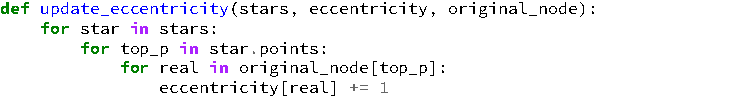
\includegraphics{assets/tmp-code/update_eccentricity.pdf}
    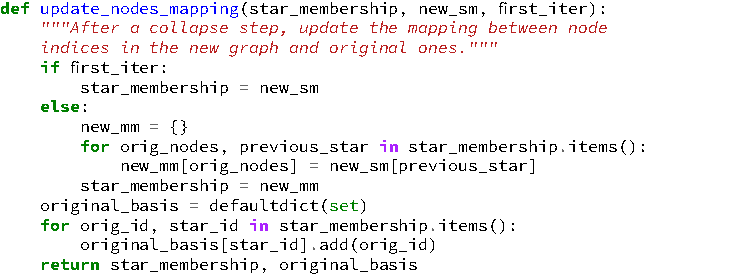
\includegraphics{assets/tmp-code/update_nodes_mapping.pdf}
    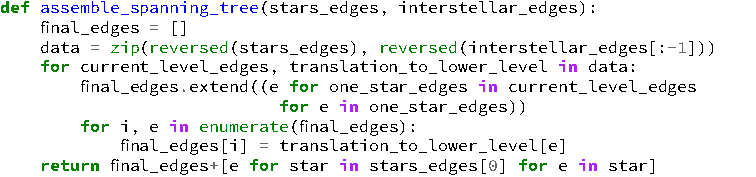
\includegraphics{assets/tmp-code/assemble_spanning_tree.pdf}
	\end{algorithmic}
\end{algorithm}

As described in \autoref{alg:gtx}, at every collapse level, we first extract stars from the current
graph (line 5), then update the eccentricity and node mappings (lines 7--8) and finally collapse the
graph (line 9). We perform these operations until there are no edge connecting stars anymore. At
this point, we revisit every outer edges to build the spanning tree (line 13).

\begin{prop}
  \label{prop:gtx_correct}
  For any connected graph $G_0$, \gtx$(G_0)$ terminates after $K\leq |V_0|$ iterations. Furthermore,
  it runs in $O(K|E_0|)$ time and returns a spanning tree of $G_0$.
\end{prop}
We will need the following lemma.
\begin{lemma}
  \label{lem:gtx_stay_connected}
  If $G_0$ is connected, then any subsequent graph $G_t,\, t \leq K$ is also connected.
\end{lemma}
\begin{proof}
 Suppose not and assume, to the contrary, that there exists at least one (or more) disconnected
 graph in $\{G_t\}_{t=1}^K$ and let $t_0$ be the smallest index such that $G_{t_0}$ is disconnected.
 Then there exist two nodes $s_u$ and $s_v$ in $V_{t_0}$ with no path between them in $E_{t_0}$.
 Letting $\mathcal{U}, \mathcal{V} \subset V_{t_0-1}$ be respectively the nodes forming stars $u$
 and $v$, this implies there is no path between nodes in $\mathcal{U}$ and nodes in $\mathcal{V}$.
 However, $G_{t_0-1}$ is connected by hypothesis, which leads to a contradiction.
\end{proof}

\begin{proof}[Proof of \autoref{prop:gtx_correct}]
  Let us first show that \gtx{} terminates in less than $|V_0|$ iterations. This follows from the
  fact that every time we collapse the graph $G_t$, we strictly reduce the number of nodes. Indeed,
  according to \autoref{lem:gtx_stay_connected}, $G_t$ is connected so at least two nodes of $V_t$
  are joined by an edge and will form a star, \ie{} a single node. We can thus claim that $|V_{t+1}| <
  |V_t|$. Note also that for all $t$, $|V_t| > 0$ and that when $|V_t|=1$, \extractStar{} creates a
  singleton and \collapseStar{} does not return any outer edges so \gtx{} finishes, proving that the
  number of iterations $K$ satisfies $K \leq |V_0|$.

 Then we analyze the time complexity. We already now that during the \tth{} iteration,
 \extractStar{} and \collapseStar{} take time $O(|E_t|)$. We provide only the actual python code
 instead of pseudo code for the remaining functions since they do not present any special
 interesting algorithmic aspect. However, we can say that \textsc{Update-Eccentricity} and
 \textsc{Update-Nodes-Mapping} take $O(|V_0|)$ time since they go through every node of the original
 graph. Because $G_0$ is connected, $|V_0| \leq |E_0|$, and since for all $t$, $|E_t| \leq |E_0|$,
 we have that the \gtx{} inner loop takes $O(K|E_0|)$ time. Finally, since
 \textsc{assemble-spanning-tree} goes again through every edge visited at every collapse step, it
 also takes $O(K|E_0|)$ time, which is thus the overall complexity of the \gtx{} algorithm.

  Finally we prove that \gtx{} indeed returns a spanning tree of $G_0$.
\end{proof}


Later we hope to found an upper bound of $T$ in terms of $m$, and also to refine the analysis to
leverage the fact that $\sum_{t=0}^T |E_t|$ is significantly smaller than $Tm$. For now, let us
prove the termination of \gtx{} by observing that, assuming $|E_t|>0$, $|E_{t+1}| < |E_t|$ since
at least two nodes in $G_t$ are connected and will therefore form a star, which will remove all the
inner edges of that star. As for the fact that we get a tree, note that a star is a tree, therefore
a star of star is a tree, and so on.\Todo{make the two arguments about \gtx{} correctness more
formal, and also explain that since all nodes are part of the ultimate star, this tree is a spanning
one. Motivate the name of \gtx{}.}

\paragraph{Example of \gtx{}}
\label{par:exemple_of_gtx}

We illustrate the operation of the \gtx{} algorithm on a small (and somewhat contrived) example.
Let us start with the initial graph $G_0$ depicted in \autoref{fig:gtx_eccentricity}
\vpageref{fig:gtx_eccentricity} and initialize
the eccentricity of all nodes to $0$. When running \extractStar{}, we see that the maximum degree is
$4$, achieved at nodes $\{1, 6, 11, 16, 21, 26, 31, 36, 41\}$. For the sake of simplicity, assume
nodes are picked according to their index. First, node $1$ forms the star $\starone{1}$ with
peripheral nodes $2$, $3$, $4$ and $5$. This increments the eccentricity of those peripheral nodes
by $1$. Then node $6$ forms its star $\starone{2}$ with $7$, $8$, $9$ and $10$. The process
continues until node $41$ is chosen to be the center of star $\starone{9}$, at which point the
max-priority queue has been exhausted and \extractStar{} finishes.

\begin{figure}[htbp]
  \centering
  \includegraphics[width=0.78\linewidth]{tikz/gtx_eccentricity_tikz.pdf}
  \caption[The hierarchical structure of stars created by \gtx{}]{%
    The execution of the \gtx{} algorithm. The original graph is made of the solid and dashed edges
    connecting the nodes labeled by their index. Edges forming the final spanning tree are solid
    while the others are dashed. Their colors indicate at which iteration they were chosen to be inside a
    star. The four shades of gray, from white to dark gray
    denote increasing node eccentricity (as computed at the end of the algorithm). The \ith{} star
    created during the \jth{} iteration of the algorithm is denoted $S_i^j$. Refer to the main text
    for the complete description of the execution.}
  \label{fig:gtx_eccentricity}
\end{figure}

\begin{figure}[bthp]
  \centering
  \begin{subfigure}[b]{0.47\textwidth}
    \centering
    \includegraphics[height=5cm]{tikz/gtx_run_level1_tikz}
    \caption{Resulting graph after the first iteration}\label{fig:gtx_run1}
  \end{subfigure}~
  \begin{subfigure}[b]{0.47\textwidth}
    \centering
    \includegraphics[height=2.2cm]{tikz/gtx_run_level2_tikz}
    \caption{Resulting graph after the second iteration}\label{fig:gtx_run2}
    \vspace{\baselineskip}
    \includegraphics[height=2.2cm]{tikz/gtx_run_level3_tikz}
    \caption{Resulting graph after the third iteration}\label{fig:gtx_run3}
  \end{subfigure}~
  \caption{The other iterations of \gtx{}}\label{fig:gtx_run}
\end{figure}

We then call \collapseStar{}. This will connect all possible pairs of star. For instance, the edge
between nodes $19$ and $29$ leads to the edge between $\starone{4}$ and $\starone{6}$. This is
actually the only possible edge between $\starone{4}$ and $\starone{6}$.  Consider on the other hand
the case of edges $(2, 6)$ and $(2, 9)$. They both connect $\starone{1}$ and $\starone{2}$. Yet at
this point of the algorithm, the eccentricity of node $2$ is $1$, the eccentricity of node $6$ is
$0$ and the eccentricity of node $9$ is $1$. The edge $(2, 6)$ has therefore the smallest total
eccentricity and is chosen to connect $\starone{1}$ and $\starone{2}$. The full result of the
\collapseStar{} procedure is $G_1$, which can be seen on \autoref{fig:gtx_run1}.

We now run \extractStar{} on $G_1$. Because all nodes have degree $2$, they could all be chosen to
be the center of a star yet we again they are picked according to their index and therefore we
choose $\starone{1}$ to be the center of the star $\startwo{1}$ with peripheral nodes $\starone{2}$
and $\starone{3}$. The original nodes belonging to those peripheral stars (nodes $4$ to $15$) have
their eccentricity incremented by $1$. The next node with highest degree in $G_1$ is now
$\starone{4}$, which forms a star with $\starone{5}$ and $\starone{6}$. This choice means that nodes
$21$ through $30$ have their eccentricity incremented by $1$. Finally, $\starone{7}$ forms the last
star with $\starone{8}$ and $\starone{9}$. Then \collapseStar{} connects the resulting three stars,
and this time there is only a single choice between each pair of stars, leading to the graph $G_2$
showed in \autoref{fig:gtx_run2}

The action of \extractStar{} on $G_2$ is quite simple, because there is only one star that can be
created, so let say we choose $\startwo{1}$ as its center, with $\startwo{2}$ and $\startwo{3}$ as
peripheral nodes. This increases the eccentricity of their underlying $G_0$ nodes by $1$ (namely
nodes $16$ to $45$). Because there is only one star $\starthree{1}$ left, \collapseStar{} returns
$G_3$ showed in \autoref{fig:gtx_run3} and an empty list of outer edges, meaning that the inner loop
of \gtx{} is finished and we can go through every edges we chose between stars at every level to
recover the final spanning tree, showed with solid edges in \autoref{fig:gtx_eccentricity}
\vpageref{fig:gtx_eccentricity}. For completeness, we can also look at the edges which are not part
of the spanning tree and therefore contribute to the stretch of the tree. In that case the average
stretch is $7$, as showed in \autoref{tab:gtx_example_stretch}.

\begin{table}[htpb]
  \centering
  \caption{Stretch of the example tree}
  \label{tab:gtx_example_stretch}
  \begin{tabulary}{\linewidth}{lLr}
    \toprule
    test edge & path in the tree & length \\
    \midrule
    $2,9$   & $2$--$6$--$9$                       & $2$ \\
    $3,12$  & $3$--$1$--$4$--$14$--$11$--$12$     & $6$ \\
    $13,29$ & $13$--$11$--$15$--$26$--$29$        & $4$ \\
    $20,24$ & $20$--$16$--$17$--$23$--$21$--$24$  & $5$ \\
    $25,42$ & $25$--$21$--$23$--$17$--$16$--$19$--$29$--$26$--$15$--$11$--$14$--$4$--$1$--$2$--$6$--$8$--$37$--$36$--$39$-- $32$--$31$--$35$--$43$--$41$--$45$ & $24$ \\
    $33,38$ & $33$--$31$--$32$--$39$--$36$--$38$  & $5$ \\
    $34,43$ & $34$--$31$--$35$--$43$              & $3$ \\
    \bottomrule
  \end{tabulary}
\end{table}

\paragraph{Number of iterations needed}\label{par:number_of_iteration}%

\textcolor{red}{\LARGE Draft}

A crucial quantity of the \gtx{} algorithm, both in terms of complexity and resulting stretch, is
the number of collapses $T$ needed before termination. While this is still elusive to express in the
general case, let us first look at some simple cases. For instance, a very sparse example of graph
is the line graph. While it is already a tree, let us look how the \gtx{} algorithm operates on it.
Say we have $n$ nodes and $m$ edges in that line. There a star is made at most of three
consecutive nodes. In the worst case, centers will be chosen such that we have a succession of three
and two nodes stars, as in \autoref{fig:gtx_line_graph}.%
\begin{marginfigure}
  \centering
  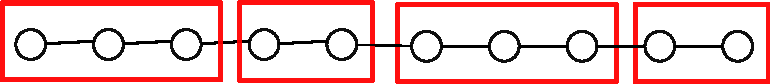
\includegraphics[width=0.9\linewidth]{assets/tmp-code/line_graph.pdf}
  \caption{A line graph with stars in red}
  \label{fig:gtx_line_graph}
\end{marginfigure}
This will results in $\nicefrac{2n}{5}$ stars, which is less than half of $n$ and because in that
case $n=m+1$, \gtx{} will finish after $O(\log m)$ iterations. Note that a barbell graph (two
cliques connected by a line) would requires a number of iterations proportional to the length of that
central line, despite having many more edges. This suggests unsurprisingly that the diameter of the graph
could be a good parameter to quantify the number of iterations needed. Indeed, take a tree and consider
the length $p$ of its longest path from the root to a leaf. By a similar argument as the one used in
the line case, it seems \gtx{} will terminate after $O(\log p)$ iterations.

While all $G_t$ are connected, it might happen during the execution of \extractStar{} that%
\begin{marginfigure}
  \centering
  \includegraphics[width=0.95\linewidth]{assets/tikz/gtx_singleton_tikz.pdf}
  \caption{The formation of a singleton star}
  \label{fig:gtx_singleton}
\end{marginfigure}
the degree of a node $u$ drops to zero because all of its neighbors were claimed by the
periphery of previous stars. Such a node then forms a \emph{singleton star}, as illustrated in
\autoref{fig:gtx_singleton}, where after the creation of \starone{1} and \starone{2}, $c_3$ is the
single node of the third star \starone{3}.%
\begin{marginfigure}
  \centering
  \includegraphics[width=0.95\linewidth]{assets/tikz/gtx_noreduc_tikz.pdf}
  \caption{A case were too many singletons \enquote{waste} one iteration of \gtx{}}
  \label{fig:gtx_noreduc}
\end{marginfigure}
In the case no singleton are formed during one execution of \extractStar{}, the number of nodes is
reduced by at least a factor $2$ (because each star is made of at least two nodes). On the other hand, we can
construct a graph with singletons where the factor of reduction in number of nodes and edges can be
arbitrarily close to $1$. Consider \autoref{fig:gtx_noreduc}, where $c_1$ and $c_2$ have a degree
$p$ and their neighbors (in light gray) all have a degree $q$, which we can vary from $1$ to $p-1$.
At this step $t$, we thus have $|V_t| = 2(1+p)+pq$ and $|E_t| = 2(p+qp)$. Next we run \extractStar{}
and assume that we first extract the two stars centered in $c_1$ and $c_2$. This reduces the
effective degree of all the middle nodes (in dark gray) to $0$ and they thus form singletons, that
are all connected to the first two stars by \collapseStar{}. As a result, at step $t+1$ we have
$|V_{t+1}| = 2 + pq$ and $|E_{t+1}| = 2pq$, so that
\begin{equation*}
\frac{|V_{t+1}|}{|V_t|} = \frac{pq+2}{p(q+2) + 2} \qquad \text{and} \qquad
\frac{|E_{t+1}|}{|E_t|} = \frac{2pq}{2p(q+1)} = \frac{q}{q+1}
\end{equation*}
When we let $p$ goes to infinity, setting $q=1$ makes $\frac{|V_{t+1}|}{|V_t|}$ tend to
$\nicefrac{1}{3}$ and $\frac{|E_{t+1}|}{|E_t|}$ to $\nicefrac{1}{2}$ while setting $q=p-1$ makes
both $\frac{|V_{t+1}|}{|V_t|}$ and $\frac{|E_{t+1}|}{|E_t|}$ tend to $1$. Note however that in both
cases, this is not really a problem because at the next iteration, there will be only two stars (one
of them will be a singleton). Is it always like that? In other words, can we have a situation where
a large number of singletons is carried over several consecutive iterations?

\paragraph{Variants of \extractStar{}}
\label{ssec:gtx_center_choice}

The execution of \extractStar{} is mainly deterministic, except for the fact the ties between nodes
with the same highest degree are broken arbitrarily. While this allows for an efficient
implementation, and simplify the analysis of the resulting sequence of stars and therefore the
induced spanning tree, in can be detrimental in an adversarial context, where we could end up with a
tree forcing a lot of mistakes. We add an element of randomization to \extractStar{} by letting it
use of two optional arguments, a \emph{threshold function} $\tau$ or a \emph{degree function}
$\widetilde{d}$. Such functions modify the center sampling process in the following way:
\begin{itemize}%[nosep]
  \item if $n_{t,i}$ is the number of node remaining in $V_t$ before choosing the \ith{} center, choose
    a node \uar{} among those with a degree larger than $\tau(n_{t,i})$. The idea is to choose
    among a small set of high degree nodes, for instance by letting $\tau(n) = \sqrt{n}$. Note
    however we cannot guarantee there will always be nodes with degree above the threshold, in which
    case we default on the highest degree node
  \item if $\degr_i(u)$ is the degree of node $u$ before choosing the \ith{} center, choose node
    proportionally to $\widetilde{d}(\degr_i(u))$. Again, the degree function is designed so that it
    favors the selection of high degree nodes. For instance, one could use
    $\widetilde{d}(\degr_i(u)) = \degr_i(u)^2$.
\end{itemize}

These two variants are more time consuming because they require additional bookkeeping.
Therefore, we don't provide a full complexity analysis and only briefly sketch their implementations
here.\footnote{Although they are available online at
\nolinkurl{https://github.com/daureg/magnet/blob/master/veverica/}%
\{\href{https://github.com/daureg/magnet/blob/master/veverica/ThresholdSampler.py}%
{ThresholdSampler.py}, \href{https://github.com/daureg/magnet/blob/master/veverica/NodeSampler.py}%
{NodeSampler.py}\}.} For the threshold function, we
maintain two queues, $high$ and $low$, containing nodes whose degree is respectively above and below
the current threshold. We select a node \uar{} in $high$, remove the corresponding star from $G_t$,
recompute the new threshold and if necessary, move nodes which fell under the threshold from $high$
to $low$ and those who climb above the threshold from $low$ to $high$. For the degree function, we
can draw any node as center proportionally to its weight (where the weight of node $u$ is defined as
$d_f\left(\degr(u)\right)$). Yet we cannot use the standard method of computing the cumulative sum
of weights since some of them change at each iteration. Therefore, we construct a binary tree whose
leaves are the nodes of $V_t$ and where each tree nodes maintain the sum of weights in its left and
right subtrees. To sample, we draw a random number $r$ between $0$ and the total weight of the tree and
go down from the root to the leaf spanning the weight interval containing $r$.
When degrees are updated (or graph node removed), we update the weights along a path from the
corresponding leaves to the root of the tree.

A variant of the \gtx{} algorithm as a whole we did not explore so much in practice is its ability
to produce spanner by stopping early. Basically if we stop at iteration $t$, we output the graph
$G_t$ (which in general is not a tree) with its edges unfolded to lie in $E_0$. This corresponds to
a trade off between having more edges than $|V_0|-1$ but potentially making shorter connection and
thus having a lower stretch.


\subsection{Related works}
\label{sub:gtx_related_works}

% \label{sub:gtx_state_of_the_art}

Looking for a subgraph $H$ of $G$ that best preserves the distance in $G$ while being sparse is an old
problem, driven originally by network design in fields such as transportation~\autocite{RoadNetworks60}
and electrical circuits~\autocite{electricalNetworks60}. The way we define \enquote{preserving the
distance}, and the exact form of $H$ give rise to several problems, which we summarize later in
\autoref{tab:gtx_related_stretch}. We first give some
definitions, then cover the most relevant problems in details, and finally give some pointers for
the others problems.

Let the distance between $u$ and $v$ in $G$ be
\begin{equation*}
  d_G(u,v) = \sum_{e \in \pathguv} \ell(e)\,,
\end{equation*}
where $\ell(e)$ is the \emph{length} of the edge $e$ and \pathguv{} is the shortest path between $u$
and $v$ in $G$. In the following, we consider only the uniform case, in which the length of an edge
is equal to its weight. The stretch of an edge $(u,v)$ in $H$ is defined as
\begin{equation*}
  \estr(u,v) = \frac{d_H(u,v)}{d_G(u,v)}.
\end{equation*}

We may then want to minimize the stretch of:
\begin{enumerate}[1),nosep]%,leftmargin=*]
  \item some pairs of nodes. That is, given $L$ and $R$ in $V$, minimize $\sum_{u \in L, v\in R}
    \estr(u,v)$
  \item all pairs of nodes corresponding to edges of $G$, \ie{} minimize $\sum_{(u,v) \in E}
    \estr(u,v)$
  \item all pairs of nodes, \ie{}  minimize $\sum_{(u,v) \in V^2} \estr(u,v)$
\end{enumerate}
Note that for unweighted graphs, the second problem reduces to minimizing
\begin{equation}
  \label{eq:test_stretch_def}
  \estr(H) = \sum_{(u,v) \in E} |\pathhuv|.
\end{equation}
If furthermore $H$ is tree, this is equivalent to minimize the second term of equation
\eqref{eq:stretch_mistakes}. Therefore we focus mainly of that definition of stretch, and consider
the other two only briefly.

The second point affecting the problem is the structure of $H$. The only requirements are that it
must be spanning all the nodes involved in the computation of the chosen stretch, and that $\forall
(u,v) \in E,\, d_H(u,v) \geq d_G(u,v)$. Beside that, $H$ can be a tree of $G$, a general subgraph of
$G$ or even a subset of $V^2$ (\ie{} containing edges not in $E$). We focus mainly on the first two
cases, since they are covered by the \gtx{} algorithm.

% Namely, let $G$ be a graph over vertex set $V$ with $|V|=n$ and edge set $E$. Furthermore, let $T$
% be a spanning tree of $G$ and $\etest{}$ the edges of $G$ not in $T$. Then we define the
% \emph{average test edge stretch} as $\frac{1}{|\etest{}|} \sum_{(u,v) \in \etest{}}
% |\mathrm{path}^T_{u,v}|$, where $|\mathrm{path}^T_{u,v}|$ is the unique path between $u$ and $v$ in
% $T$.


% However, \textcite[Section 3, page 453]{lognMetricBoundConf03} claim a $O(\log n)$ approximation so maybe I'm
% wrong. Turns out, they refer to a distribution over trees and this $O(\log n)$ is the expected
% stretch of a tree sampled from this distribution

% This defines two kind of structures, spanning trees and spanners (which are still sparse subgraphs
% yet containing more than $|V|-1$ edges).

\paragraph{Trees}
\label{par:trees}

One early mention of seeking a low-stretch spanning tree is given by \textcite{Requirements74},
albeit in more general form:
\begin{problem}[Optimal Communication Spanning Tree]
Given a set of nodes $V=\{v_1, \ldots, v_n\}$, a set of distances $d_{ij}$ and a set of requirements
$r_{ij}$ between $v_i$ and $v_j$, find a spanning tree connecting these $n$ nodes such that the
total cost of communication of the spanning tree is a minimum among all spanning trees. The cost of
communication for a pair of nodes is $r_{i,j}$ multiplied by the sum of the distances of arcs which
form the unique path connecting $v_i$ and $v_j$ in the spanning tree. The cost of a spanning tree is
the sum of costs over all pairs of nodes.
\end{problem}
For a weighted graph $G=(V,E,w)$, by letting $d_{ij} = w_{ij}$ and $r_{i,j}= \Ind{(i,j) \in E}$,
finding an Optimal Communication Spanning Tree thus amounts to finding a low-stretch spanning tree.
\autoref{tab:gtx_related} present a list of works where the stretch was improved.

We start with the seminal paper of \textcite{LowerBound95}. It touches on many topics, and frame the
problem in a game theoretic way but here we only focus on two of their results: a lower bound of
$\Omega(\log n)$ for the average stretch of any tree and their construction of a tree with $\exp
O(\sqrt{\log n\log\log n})$ average stretch in time $O(m^2)$. The lower bound follows from an
existing result in extremal graph theory~\autocite[pages 107--109]{ExtremalGraph04}: there is a
positive constant $a$ such that for all $n\in \Nbb$, one can construct a graph $G$ with $n$ vertices
and $2n$ edges such that every cycle $G$ has a length of at least $a\log n$. Now consider any
spanning tree $T$ of $G$.  While all the $n-1$ edges of $T$ have a stretch of $1$, the $n+1$
remaining ones form a cycle in $T$ hence in $G$ as well and thus incur a stretch of at least $a\log
n$. This shows that the average stretch is at least $\frac{1}{2}a\log n$.

They construct a low stretch spanning tree in a bottom up manner like the \gtx{} algorithm. First,
they extend the definition of stretch to multigraph~\autocite[Section 4]{LowerBound95} and then
describe a procedure to transform in linear time any multigraph $G$ with $n$ nodes to a multigraph
$G'$ on the same nodeset with at most $n(n+1)$ edges such the average stretch of $G'$ is at most
twice that of $G$~\autocite[Lemma 5.2]{LowerBound95}. The next ingredient is an algorithm to build a
low diameter decomposition of a multigraph $G$, parametrized by a number $x(n)$ depending of $n$. It
works by repeatedly selecting an arbitrary node and growing a ball around it until the number of
edges leaving the ball is at most a fraction $\nicefrac{1}{x(n)}$ of the number of edges with both
endpoints in the ball. The key property of this decomposition is that it yields a partition of $G$
in clusters such that the radius of each cluster is small (namely at most $O(x(n)\log n)$) and there
is most a fraction $\nicefrac{1}{x(n)}$ of edges between clusters. Finally, the iterative procedure
is a follows: once a partition has been built, we compute a shortest path spanning tree in each
cluster that are then collapsed into super nodes to form the next graph $G'$ and the process repeats.
Another difference from \gtx{}, besides the partition procedure, is that $G'$ is a multigraph,
taking into account the number of edges joining cluster, while \collapseStar{} picks only the most
direct one.

Another interesting idea from this paper is to consider a distribution over trees instead of a
single instance, especially when one is concerned about the maximum stretch instead of the average
one. For instance, on a cycle with $n$ nodes, a tree is obtained by removing one edge, and that edge
incurs a stretch of $n-1$. The uniform distribution over such trees has a maximum stretch of
$2\left(1 - \frac{1}{n}\right)$~\autocite{circle2k89}.

\begin{table}[htbp]
  \centering
  \caption{Reproduction of Table 1 from~\autocite{Abraham2012}, showing the evolution of the best
  asymptotic average stretch over time.}\label{tab:gtx_related}
  \begin{tabular}{lll}
    \toprule
    work                      & average stretch                          & time                    \\
    \midrule
    \autocite{LowerBound95}   & $\exp(O(\sqrt{\log n\log\log n}))$       & $O(m^2)$                \\
    \autocite{LowerStretch05} & $O((\log n)^2 \log \log n)$              & $O(m \log^2 n)$         \\
    \autocite{nearlyTight08}  & $O(\log n(\log \log n)^3)$              & $O(m \log^2 n)$         \\
    % \autocite{nearlyTight08}  & $O(\log n \log\log n(\log\log\log n)^3)$ & $O(m^2)$                \\
    \autocite{TighterSDD11}   & $O(\log n(\log \log n)^3 )$              & $O(m \log n\log\log n)$ \\
    \autocite{Abraham2012}    & $O(\log n \log \log n)$                  & $O(m \log n\log\log n)$ \\
    \bottomrule
  \end{tabular}
\end{table}

The idea of recursively partitioning the graph and construction a low-stretch spanning tree in each
part is common to all the papers of \autoref{tab:gtx_related}. \Textcite{LowerStretch05} devise a
$(\delta, \epsilon)$-star decomposition such that all the stars have comparably low radius.
It was modified in~\autocite{nearlyTight08} to improve the stretch. Then \textcite{TighterSDD11}
improve the runtime by rounding the edge weights to the closest power of $2$ and using a modified
implementation of the Dijkstra's algorithm in the case of at most $k$ distinct edge
weights~\autocite{FastPathFewWeights10}. Finally, \textcite{Abraham2012} describe an even more
complex but tighter petal decomposition.
\iffalse
\begin{marginfigure}
  \centering
  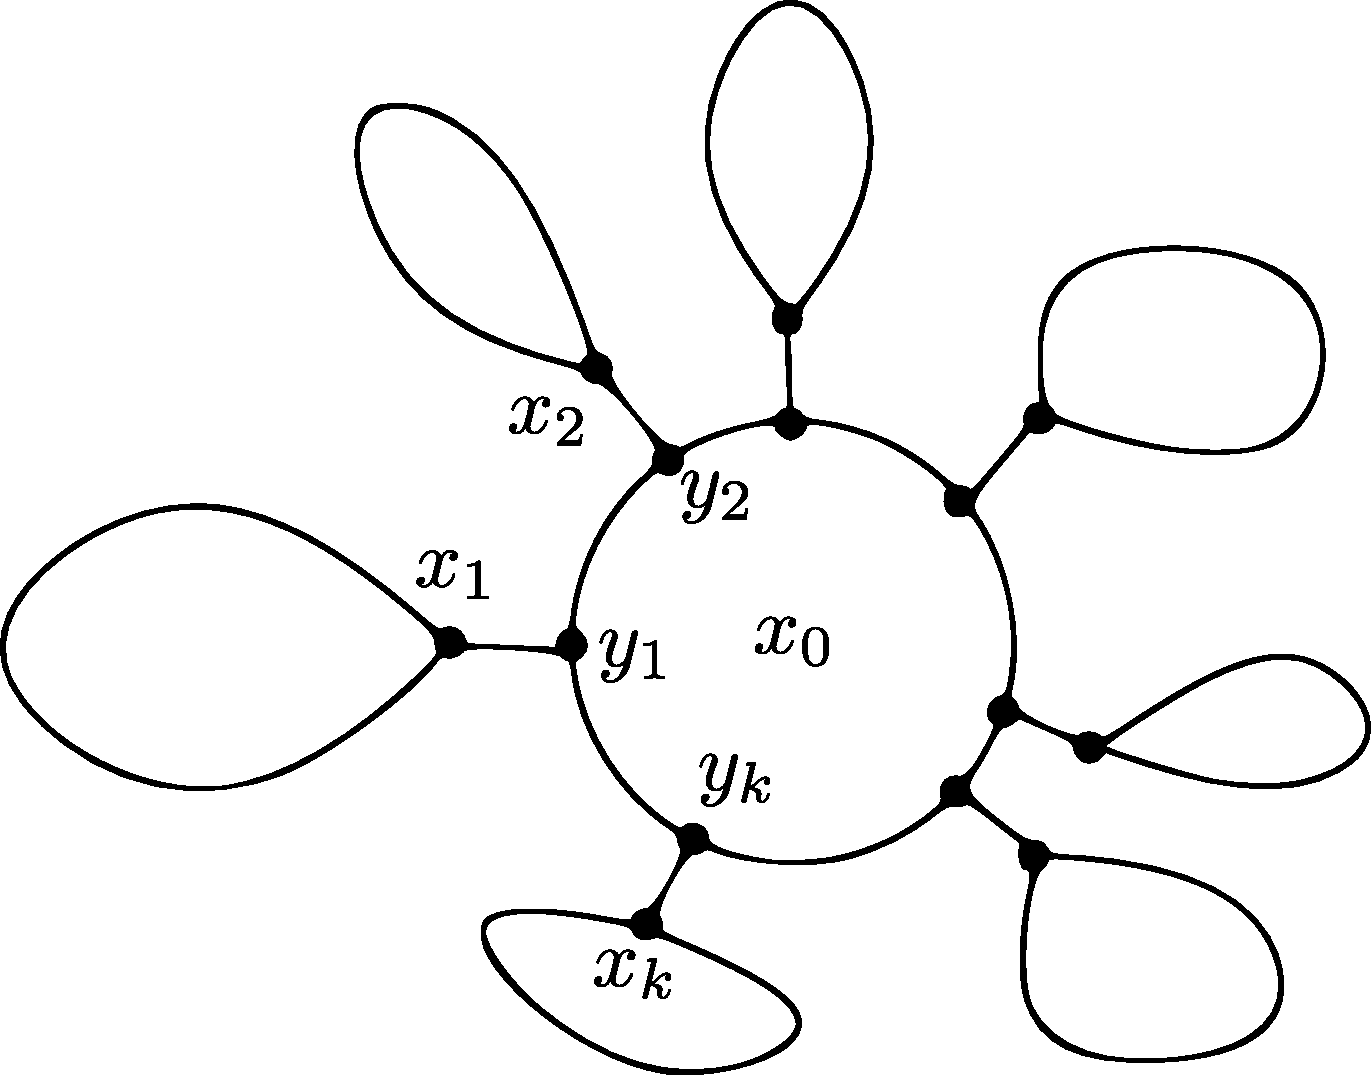
\includegraphics[width=.95\textwidth]{assets/raw/star_decomp.pdf}
  \caption{Star decomposition (reproduced from Figure 1 of~\autocite{LowerStretch05})}
  \label{fig:gtx_star_decomp}
\end{marginfigure}

Special case of graph
series parallel
\enquote{In a subsequent paper, \textcite{seriesParallel06} proved that every series-parallel
unweighted graph admits a spanning tree of average stretch $O(log n)$. This bound is tight as it
matches the lower bound established in~\autocite{cutsTrees99}.}

more special cases are in~\autocite{specialCase14}, although it's for the minimum max stretch
$t^\star$.
\enquote{Note also that a number of particular graph classes (like interval
graphs, permutation graphs, asteroidal-triple–free graphs, strongly chordal graphs,
dually chordal graphs, and others) admit tree $t$-spanners for small values of $t$}
\fi


\paragraph{Spanners}
\label{par:spanners}

As we mentioned, by stopping the \gtx{} algorithm before it finishes, we obtain a set of edges
spanning the graphs that is not a tree. Such structure are called \emph{spanner}. More precisely,
the subgraph $H$ is said to be an $t$-spanner of $G$ if, for a parameter $t \geq 1$, and for every
pair $u, v \in V$ of vertices, it holds that $d_H(u, v) \leq t \cdot d_G(u, v)$. The problem was
introduced by \textcites{SpannerFirst89}{SpannerSecond89} and has been extensively studied since
then, for it has many applications in network design. It was also showed to be \NPh{} to
approximate~\autocite{SpannerNPHard07}. The most simple construction is a greedy
algorithm~\autocite{greedySpanner93} that works similarly to the minimum spanning tree construction.
Starting from an empty subgraph $H$, it goes through every edge $(u, v)$ of $G$ sorted by weight and
check if there is a path between $u$ and $v$ in $H$ of length at most $t$. If this is the case, the edge
$(u,v)$ is dropped, otherwise it is inserted in $H$. This results in a $(2t - 1)$-spanner with
$O(n^{1+1/t})$ edges, which is an optimal trade-off between those two quantifies.  Furthermore on
weighted graphs, the greedy spanner total weight is essentially optimal~\autocite{GreedyOpt16}.
However, the best implementation of it, using a dynamic data structure~\autocite{fastGreedy04} is
not scalable for it runs in $O(t n^{2+\nicefrac{1}{t}})$ and cannot easily be parallelized.
Parallelization therefore requires other kind of approaches~\autocites{parSpanner08}{parSpanner15}.
Recently, \textcite{Spanner17} showed how to obtain, for any $\epsilon > 0$, a $(2t - 1)$-spanner
with $O(n^{1+1/k}/\epsilon)$ edges in $t$ rounds, with probability at least $1 - \epsilon$.

\iffalse
\url{http://www.siam.org/meetings/da17/schedule.html} SODA 13B \url{http://dl.acm.org/citation.cfm?id=3039686}
for instance the Elkin paper~\autocite{Spanner17} \enquote{Our centralized randomized algorithm computes (with
probability close to 1), a $(2k - 1)$-spanner with $n \cdot (1 + O(\frac{\log k}{n}))$ edges in
$O(|E|)$ time, whenever $k = \Omega(\log n)$. Note that when $k = \omega(\log n)$, the number of
edges is $n(1+o(1))$, i.e., in this range the algorithm computes an ultra-sparse spanner in $O(|E|)$
time.} For instance, if $k=5\log n$, we get a $10\log n$-spanner with $n\left(1+O\left(\frac{\log\log
n}{n}\right)\right)$ edges in $O(|E|)$ time.


They have applications in computing approximately shortest
paths [9, 22, 28, 37], routing [48], distance oracles and
labeling schemes [49, 56, 36] and synchronization [7].

From 6:They also appear in biology in the process of reconstructing phylogenetic trees from
matrices, whose entries represent genetic distances among contemporary living species (H. J.
Bandelt, A. W. M. Dress, Reconstructing the Shape of a Tree from Observed Dissimilarity Data, Adv.
in Appl. Math. 7 (1986)). Robotics researchers have studied spanners under the constraints of
Euclidean geometry, where vertices of the graph are points in space, and edges are line segments
joining pairs of points (Chew), (Dobkin), $[DJ], [K], [KG], [LL]$. 

studied in 1; 4; 6; 9; 15; 19; 22; 24; 26; 28; 30; 31; 37; 43; 51; 52; 57; 58



\begin{tabulary}{\textwidth}{LLLLL}
  \toprule
  work  & average stretch & edge size                              & weighted & time                                             \\
  \midrule
  46    & $4k + 1$        & $O(n^{1+\nicefrac{1}{k}})$             & no       & polynomial                                       \\
  6     & $2k +1$         & $O(n\cdot \ceil{n^{\nicefrac{1}{k}}})$ & yes      & $O\left(m(n^{1+\nicefrac{1}{k}}+n\log n)\right)$ \\
  40    & $2k-1$          & $O(n^{1+\nicefrac{1}{k}}+n)$           & no       & $O(m)$                                           \\
  Elkin & $2k-1$          & $n \cdot (1 + O(\frac{\log k}{n}))$    & no       & $O(m)$                                           \\
  \bottomrule
\end{tabulary}

% 22: E. Cohen, "Fast algorithms for constructing t-spanners and paths with stretch t," Proceedings
% of 1993 IEEE 34th Annual Foundations of Computer Science, Palo Alto, CA, 1993, pp. 648-658.  doi:
% 10.1109/SFCS.1993.366822
% We construct t-spanners of size (number of edges) Õ(n 1+(2+\epsilon)/t )
% (for any \epsilon > 0 and t such that t/(2+\epsilon) is integral). These spanners can be constructed
% by a randomized algorithm that runs in Õ(mn (2+\epsilon)/t ) time.


% Halperin and Zwick [40].  Their deterministic algorithm, for an integer parame- ter k ≥ 1,
% computes a (2k − 1)-spanner with n 1+1/k + n edges in O(|E|) time. (Their result improved previous
% pioneering work by [46, 22].)

Describe the greedy algorithm of 6. Using (55 On Dynamic Shortest Paths Problems Liam Roditty, Uri
Zwick, 2004), it runs in $O(\alpha n^{2+\nicefrac{1}{\alpha}})$

peleg 2007 hardness results

46: Peleg, D. and Schäffer, A. A. (1989), Graph spanners. J. Graph Theory, 13: 99–116.
doi:10.1002/jgt.3190130114

study the problem on unweighted graph. Application to routing scheme (48: D. Peleg and E. Upfal, A
tradeoff between space and efficiency for routing tables. 20th ACM Symposium on the Theory of
Computing, Chicago (1988))
Special case for the complete graph weighted by the distance in a 2D plan. Existing $\sqrt{10}$
spanner for the $\ell_1$ metric (L. P. Chew, There is a planar graph almost as good as the complete
graph.  Proceedings of the 2nd ACM Symposium on Computational Geometry, (1986)) (improved to
$\sqrt{4+2\sqrt{2}}$ by N. Bonichon, C. Gavoille, N. Hanusse, L. Perkovic The stretch factor of
$\ell_1$ and $\ell_{\infty}$ Delaunay triangulations European Symposium on Algorithms (ESA) (2012))
and $\phi \pi$ for $\ell_2$ (D. P. Dobkin, S. J. Friedman, and K. J. Supowit, Delaunay graphs are
almost as good as complete graphs. 28th IEEE Symposium on the Foundations of Computer Science,
(1987)) (improved to $1.998$ by Ge Xia. 2011. Improved upper bound on the stretch factor of delaunay
triangulations. In Proceedings of the twenty-seventh annual symposium on Computational geometry
(SoCG '11)). See (Prosenjit Bose, Michiel Smid, On plane geometric spanners: A survey and open
problems, Computational Geometry, Volume 46, Issue 7, 2013) for more on the 2D case.

In undirected graph, finding a spanner with less than $k$ edges is \NPc{} (theorem 2.2)
For $k<n$, one can construct in polynomial time a $(4\log_k n +1)$ spanner with less than $kn$ edges
(theorem 2.4) giving for instance ($k=2$) $O(\log n)$ spanner with $O(n)$ edges and
($k=n^{\nicefrac{1}{r}}$, $r\geq 1$) a $(4r+1)$ spanner with $O(n^{1+\nicefrac{1}{r}})$ edges
(matching lower bound within constant factor). For every $d \geq 0$, the $d$-dimensional cube has a
$3$-spanner with fewer than $7\time 2^d$ edges (Lemma 2.10 from 47: D. Peleg and J. D. Ullman. An
optimal synchronizer for the hypercube. SIAM J. on Comput., 18:740–747, 1989)
For chordal graphs: for every $n$-vertex chordal graph there exists a $2$-spanner with
$O(n\sqrt{n})$ edges (matching lower bound), a $3$-spanner with $O(n \log n)$ edges and a $5$-spanner
with $O(n)$ edges.
Much more difficult for directed graph, according to Theorem 4.2: For every $t \geq 1$ there are
infinitely many $n$-vertex directed graphs for which every $t$-spanner requires
$\Omega(\nicefrac{n^2}{t^2})$ edges.

% check some surveys of the 80's
% http://pubsonline.informs.org/doi/abs/10.1287/trsc.18.1.1
% http://onlinelibrary.wiley.com/doi/10.1002/net.3230190305/full
% early solutions
% http://onlinelibrary.wiley.com/doi/10.1002/net.3230090104/full
% http://onlinelibrary.wiley.com/doi/10.1002/net.3230130309/full
% later solution?
% http://ieeexplore.ieee.org/document/81738


While they have many applications [see first paragraph of \url{https://arxiv.org/pdf/1401.2454.pdf},
which was later merged in a STOC'14 paper] (a major one being solving linear systems), in some
practical situations their advantages are less clear [from
\url{https://link.springer.com/chapter/10.1007/978-3-319-20086-6_16}\enquote{for reasonable inputs
the constant factors make the solver much slower than methods with higher asymptotic complexity.
One other aspect predicted by theory is confirmed by our findings: Spanning trees with lower
stretch indeed reduce the solver's running time. Yet, simple spanning tree algorithms perform
better in practice than those with a guaranteed low stretch.} this is improved by
\url{https://link.springer.com/chapter/10.1007%2F978-3-319-20086-6_17} although they seem to work
	mostly with the Laplacian of the tree ]
\fi

\paragraph{Other problems}

Finding low stretch trees and spanners with respect to the existing edges is the most relevant
problem when addressing the \esp{} problem. For the sake of completeness, we nonetheless give an
overview of some related problems.

For instance, \textcite{Johnson1978} define the following problem, where the stretch is defined over
all possible pairs of nodes\footnote{We adapt their notations
to match ours}:  
\begin{problem}[Network Design Problem]
  \label{prob:gtx_ndp}
  Given an undirected integer-weighted graph $G=(V, E, w)$, a budget $B\in\Nbb$ and a criterion
  threshold $C\in \Nbb$, does there exist a spanning subgraph $G'=(V, E')$ of $G$ with weight
  $w(E') \leq B$ and criterion value $F(G') \leq C$, where the criterion function $F(G')$ denotes
  the sum of the weights of the shortest paths in $G'$ between all vertex pairs?
\end{problem}
They prove that finding such a subgraph is \NPc{}, by exhibiting a reduction from the
\textsc{Knapsack} problem. They also prove that the less general problem of finding a spanning tree
on an unweighted graph, that is
\vspace{-.5\baselineskip}
\begin{problem}[Simple Network Design Problem]
  \autoref{prob:gtx_ndp} with $w$ being the equal to $1$ for all edges in $E$ and $B=|V|-1$.
\end{problem}%
\vspace{-.5\baselineskip}
\noindent is also \NPc{} by reduction from \textsc{Exact 3-Cover}.
However, it has recently been show that this Simple Network Design problem can be approximated to a
constant factor $6$~\autocite{AllPairStrech10}. Moreover, even when the graph is weighted,
\textcite{constantDistortion07} achieve a universal constant bound for any weighted graph.

Another problem appear when the low-stretch structure $H$ can include edges not in $G$ (as long as
the distances in $H$ remain larger than the distances in $G$). This is captured by the following
problem~\autocite{OptimalNetwork69}:
\begin{problem}[Optimal Network Problem]
  \label{prob:gtx_scott}
  Given a set $V$ of $n$ vertices, find a set of spanning edges $E\subset V^2$ that minimizes
  the sum of the length of the shortest paths  between all vertex pairs while the
  total length of the resulting network does not exceed some upper bound $B\in\Nbb$.
\end{problem}
This can be seen as a special case of \autoref{prob:gtx_ndp} with $G$ being the unweighted
$n$-complete graph. \Textcite{OptimalNetwork69} proposes a backtracking solution and two local search approximate
algorithms. Some early branch and bound heuristic solutions to \autoref{prob:gtx_scott} are surveyed
in~\autocite[Section 2.3.2]{networkDesignSurvey89} although they do not come with asymptotic
guarantee on the stretch. Furthermore, \textcite{optimApproxNP80} proves that for any $\epsilon \in
(0,1)$, finding a $|V|^{1-\epsilon}$ approximation is \NPc{}.
However, if we consider the average stretches over a distribution of trees, then this approximation
factor can be reduced to $\Theta(\log n)$~\autocite{lognMetricBoundConf03}.

Finally, the stretch can also be computed for a subset of the edges. This is useful in cases where
we have prior information on the importance of individual nodes or edges.  For instance,
\textcite{RamseyTree17} show that for every $t$, any $n$-nodes graph $G=(V,E)$ has a subset $S$ of
size at least $n^{1 - \nicefrac{1}{k}}$, and a spanning tree that has stretch $O ( k \log \log n)$
between any node in $S$ and any node in $V$. Likewise, \textcite{mLAST17} describe how to maintain a
light subgraph $H$ that minimizes the distance between pairs of source and sink that are given in an
online fashion.

As shown by \autoref{tab:gtx_related_stretch}, those problems defined in the seventies are still
being discussed nowadays in top tier conferences, proving their relevance and impact beyond the
\esp{} problem.

\setlength{\fullpage}{179mm}
\begin{table}[htbp]
\begin{adjustwidth}{-2cm}{}
  \centering
  \caption{A summary of the lowest stretches achievable for various problems.
  \label{tab:gtx_related_stretch}}
  \begin{tabulary}{\fullpage}{LCCL}
    \toprule
    kind of stretch    & \multicolumn{2}{c}{only existing edges}  & extra edges allowed   \\
    \midrule
                       & tree                                     & not tree             &\\
    \cmidrule(r){2-3}
    some pairs         & $O(k\log\log n)$~\autocite{RamseyTree17} & \autocite[Section 4]{mLAST17} & --- \\
    all existing pairs & $O\left(\log n (\log\log n)\right)$~\autocite{Abraham2012}
		       & $(2t - 1)$-spanner, $O(n^{1+1/t})$ edges~\autocite{greedySpanner93}
		       & $\Theta(\log n)$ in expectation~\autocite{lognMetricBoundConf03} \\
    all possible pairs & $6$ for unweighted graphs \autocite{AllPairStrech10} and $O(1)$
                         in general \autocite{constantDistortion07}
		       & ---
		       & no need for extra edges in that case                              \\
    \bottomrule
  \end{tabulary}
\end{adjustwidth}
\end{table}


\url{http://www.siam.org/meetings/da17/schedule.html} SODA 13B \url{http://dl.acm.org/citation.cfm?id=3039686}
for instance the Elkin paper \enquote{Our centralized randomized algorithm computes (with
probability close to 1), a $(2k - 1)$-spanner with $n \cdot (1 + O(\frac{\log k}{n}))$ edges in
$O(|E|)$ time, whenever $k = \Omega(\log n)$. Note that when $k = \omega(\log n)$, the number of
edges is $n(1+o(1))$, i.e., in this range the algorithm computes an ultra-sparse spanner in $O(|E|)$
time.} For instance, if $k=5\log n$, we get a $10\log n$-spanner with $n\left(1+O\left(\frac{\log\log
n}{n}\right)\right)$ edges in $O(|E|)$ time.

While they have many applications [see first paragraph of \url{https://arxiv.org/pdf/1401.2454.pdf},
which was later merged in a STOC'14 paper] (a major one being solving linear system), in some
practical situations their advantages are less clear [from
\url{https://link.springer.com/chapter/10.1007/978-3-319-20086-6_16}\enquote{for reasonable inputs
the constant factors make the solver much slower than methods with higher asymptotic complexity.
One other aspect predicted by theory is confirmed by our findings: Spanning trees with lower
stretch indeed reduce the solver's running time. Yet, simple spanning tree algorithms perform
better in practice than those with a guaranteed low stretch.} this is improved by
\url{https://link.springer.com/chapter/10.1007%2F978-3-319-20086-6_17} although they seem to work
	mostly with the Laplacian of the tree ]
\fi

\subsection{Empirical evaluation}
\label{sub:gtx_empirical_evaluation}

% In this section, we provide empirical evidences of the properties of
\gtx{} over several classes of graph, and compare it with a \bfs{} baseline.
%\marginpars{If time allows, it would be interesting to implement some methods of \vref{sub:gtx_state_of_the_art} and add them to the comparison}\todo*{implement more low stretch methods}
Namely, we consider three kinds of
graph topology (with both synthetic and real world instances that carry signs on their edges) and
evaluate $(i)$ what average stretch is reached by various trees and $(ii)$ how accurate is the sign
prediction.

\subsubsection{Graph topology}

The three kinds of topology we consider are:
\begin{description}[leftmargin=*]
	\item[\grid{}] which are 2D lattices, where each node has four neighbors except on the boundary.
		The synthetic ones are square, while the \enquote{real world} ones represents the four neighbors
		pixel connectivity of the pictures showed in \autoref{fig:gtx_xp_bwpics}.
	\item[\lpa{}] which are built synthetically according to the model of \textcite{Barabasi1999}.
		While this does not follow the more rigorous specification of \textcite{PAmodel04}, informally,
		we start with a line graph of $m$ nodes and add node one by one until the graph consists of $n$
		nodes. Each time a new node is added, it is connected to $m$ of the existing nodes with a
		probability proportional to their degree. Here we choose $m=3.13$, that is when adding a new
		node, we pick $3$ or $4$ existing neighbors such the initial expected number of neighbors for
		each new nodes is $3.13$. Such graphs are quite sparse and have short diameter, thus providing a
		crude but reasonable approximation of online social networks. Therefore, the real world
		instances of the \lpa{} model are \wik{}, \sla{} and \epi{} networks from \autoref{chap:troll}
		 along with \gplus{}. The last one is constructed from
		ego networks of \gplus{}\footnote{Available at
		\url{http://snap.stanford.edu/data/egonets-Gplus.html}} by keeping the largest connected
		component of users whose gender is known. Basic statistics of those real \lpa{} graphs are
		presented in (\autoref{tab:gtx_xp_dataset}). 
	\item[\triangle{}] which consists of a Delaunay triangulation of a set of points randomly
		located in a 2D space.\footnote{As
		implemented by the \textsf{graph-tool} library (\url{https://graph-tool.skewed.de})}
\end{description}

\begin{table}[htpb]
	\centering
	\caption{Dataset description }\label{tab:gtx_xp_dataset}
	\begin{tabular}{lrrcc}
		\toprule
             & $|V|$  & $|E|$    & fraction of $+$ edges & $\frac{2|E|}{|V|\cdot(|V|-1)}$ \\
		\midrule
		\wik{}   & \np{7065}   & \np{99936}    & 78.5\%                & $4.00\cdot 10^{3}$             \\
		\gplus{} & \np{74917}  & \np{10130461} & 67.6\%                & $3.61\cdot 10^{3}$             \\
		\sla{}   & \np{82052}  & \np{498527}   & 76.4\%                & $1.48\cdot 10^{4}$             \\
		\epi{}   & \np{119070} & \np{701569}   & 83.2\%                & $9.90\cdot 10^{5}$             \\
		\bottomrule
	\end{tabular}
\end{table}

\begin{figure}[t]
	\centering
	\begin{subfigure}[b]{0.32\textwidth}
		
\includegraphics[width=\textwidth]{gtx_exp/zmonastery}
	\end{subfigure}~
	\begin{subfigure}[b]{0.32\textwidth}
		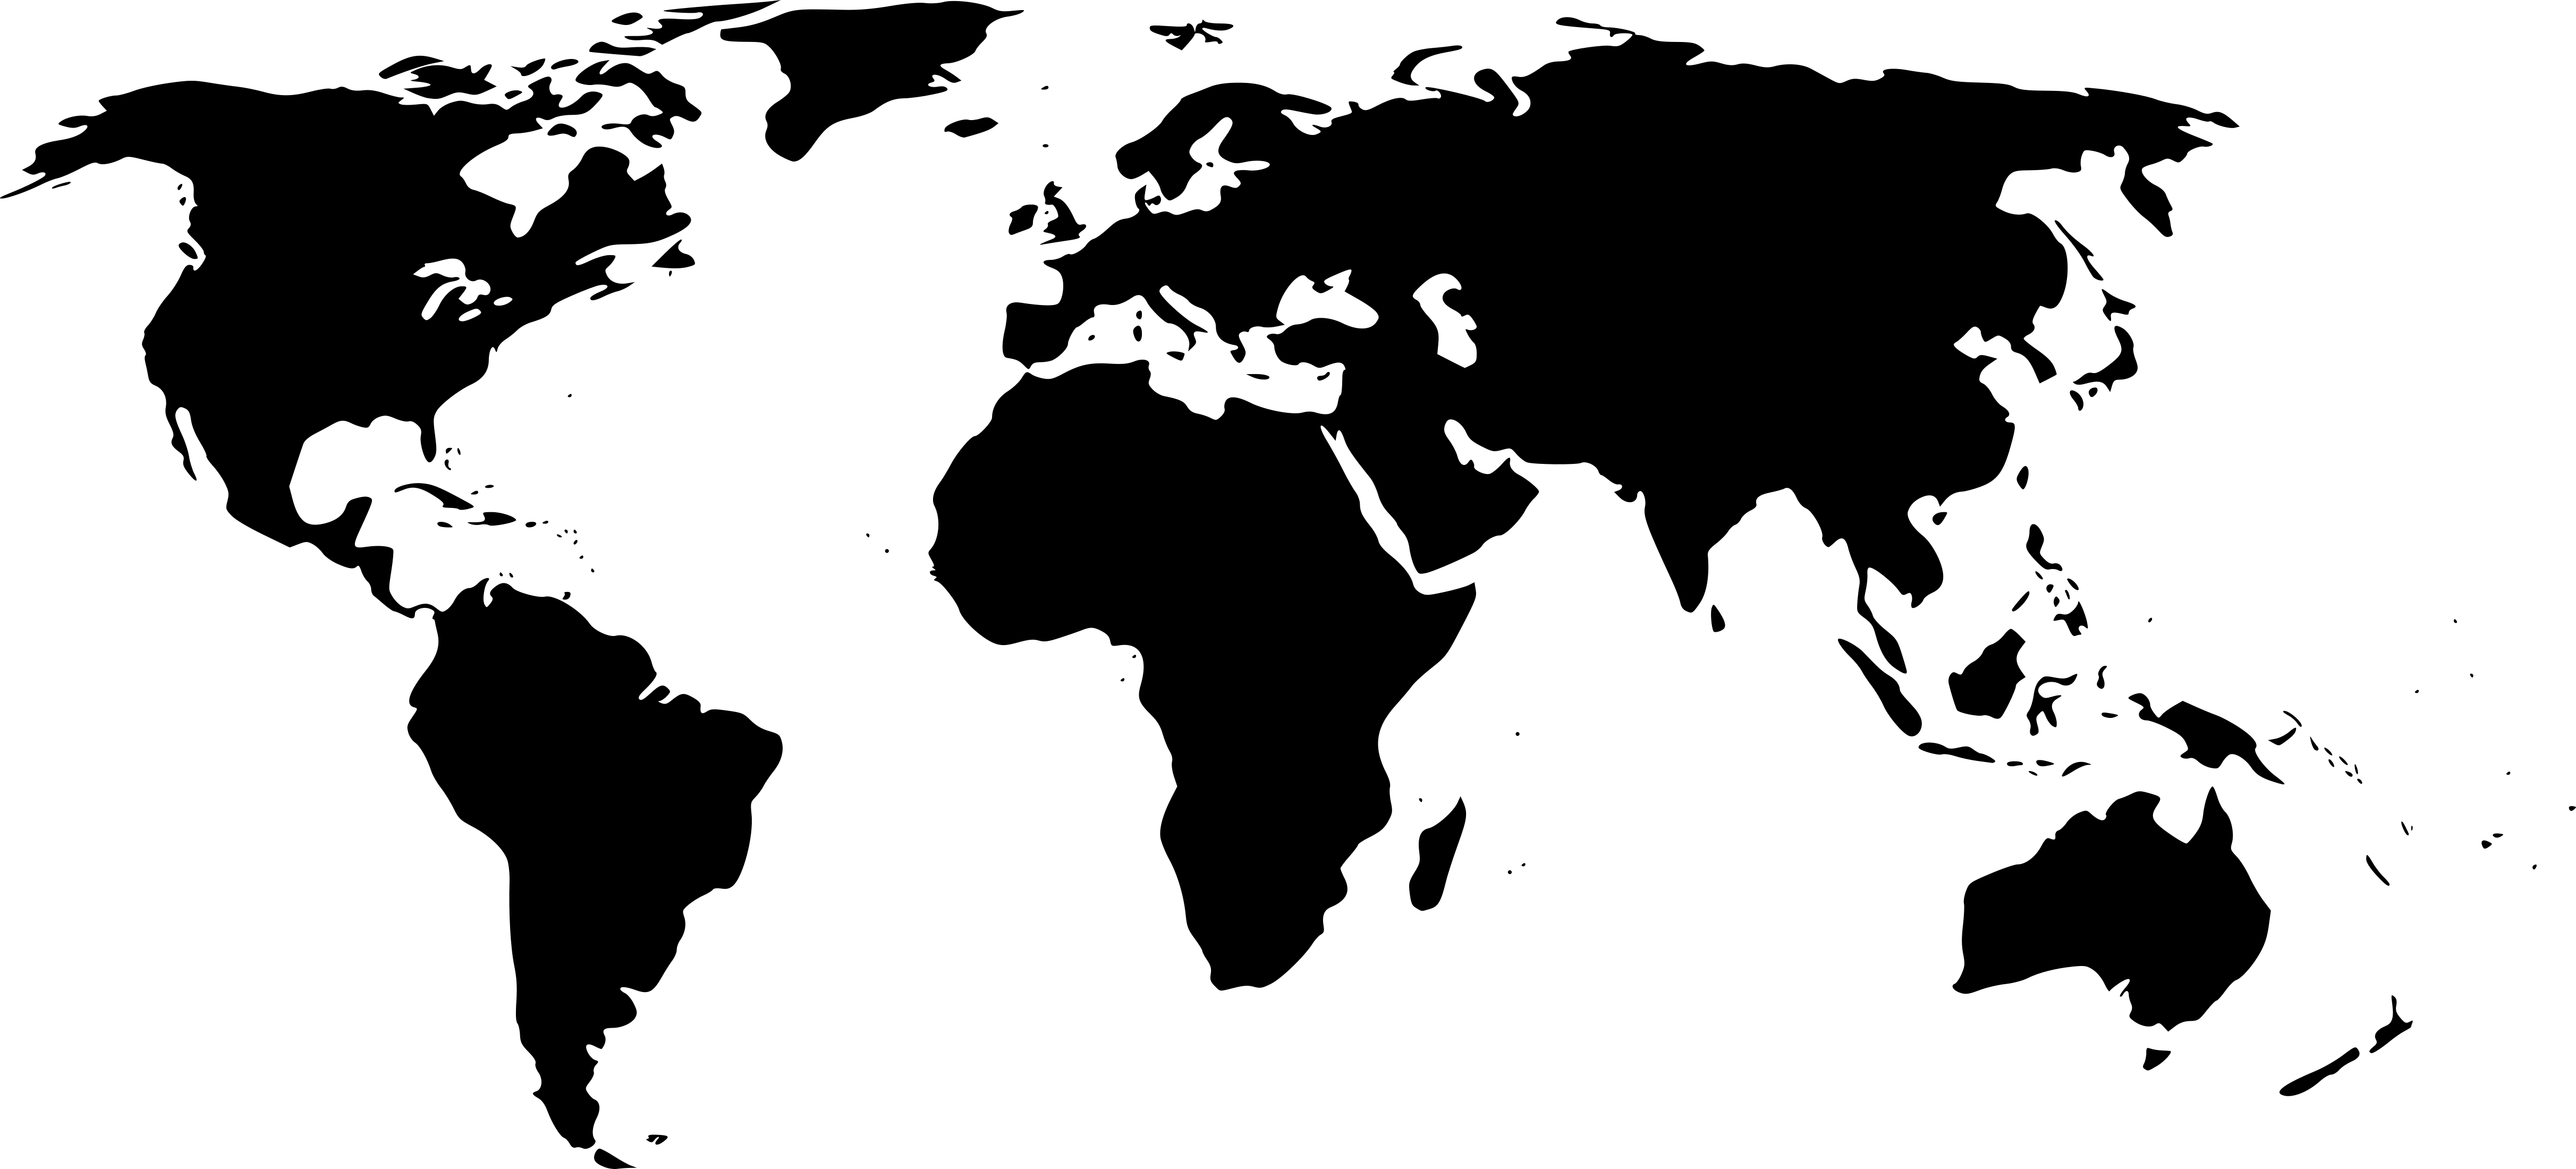
\includegraphics[width=\textwidth]{gtx_exp/zworld}
	\end{subfigure}~
	\begin{subfigure}[b]{0.32\textwidth}
		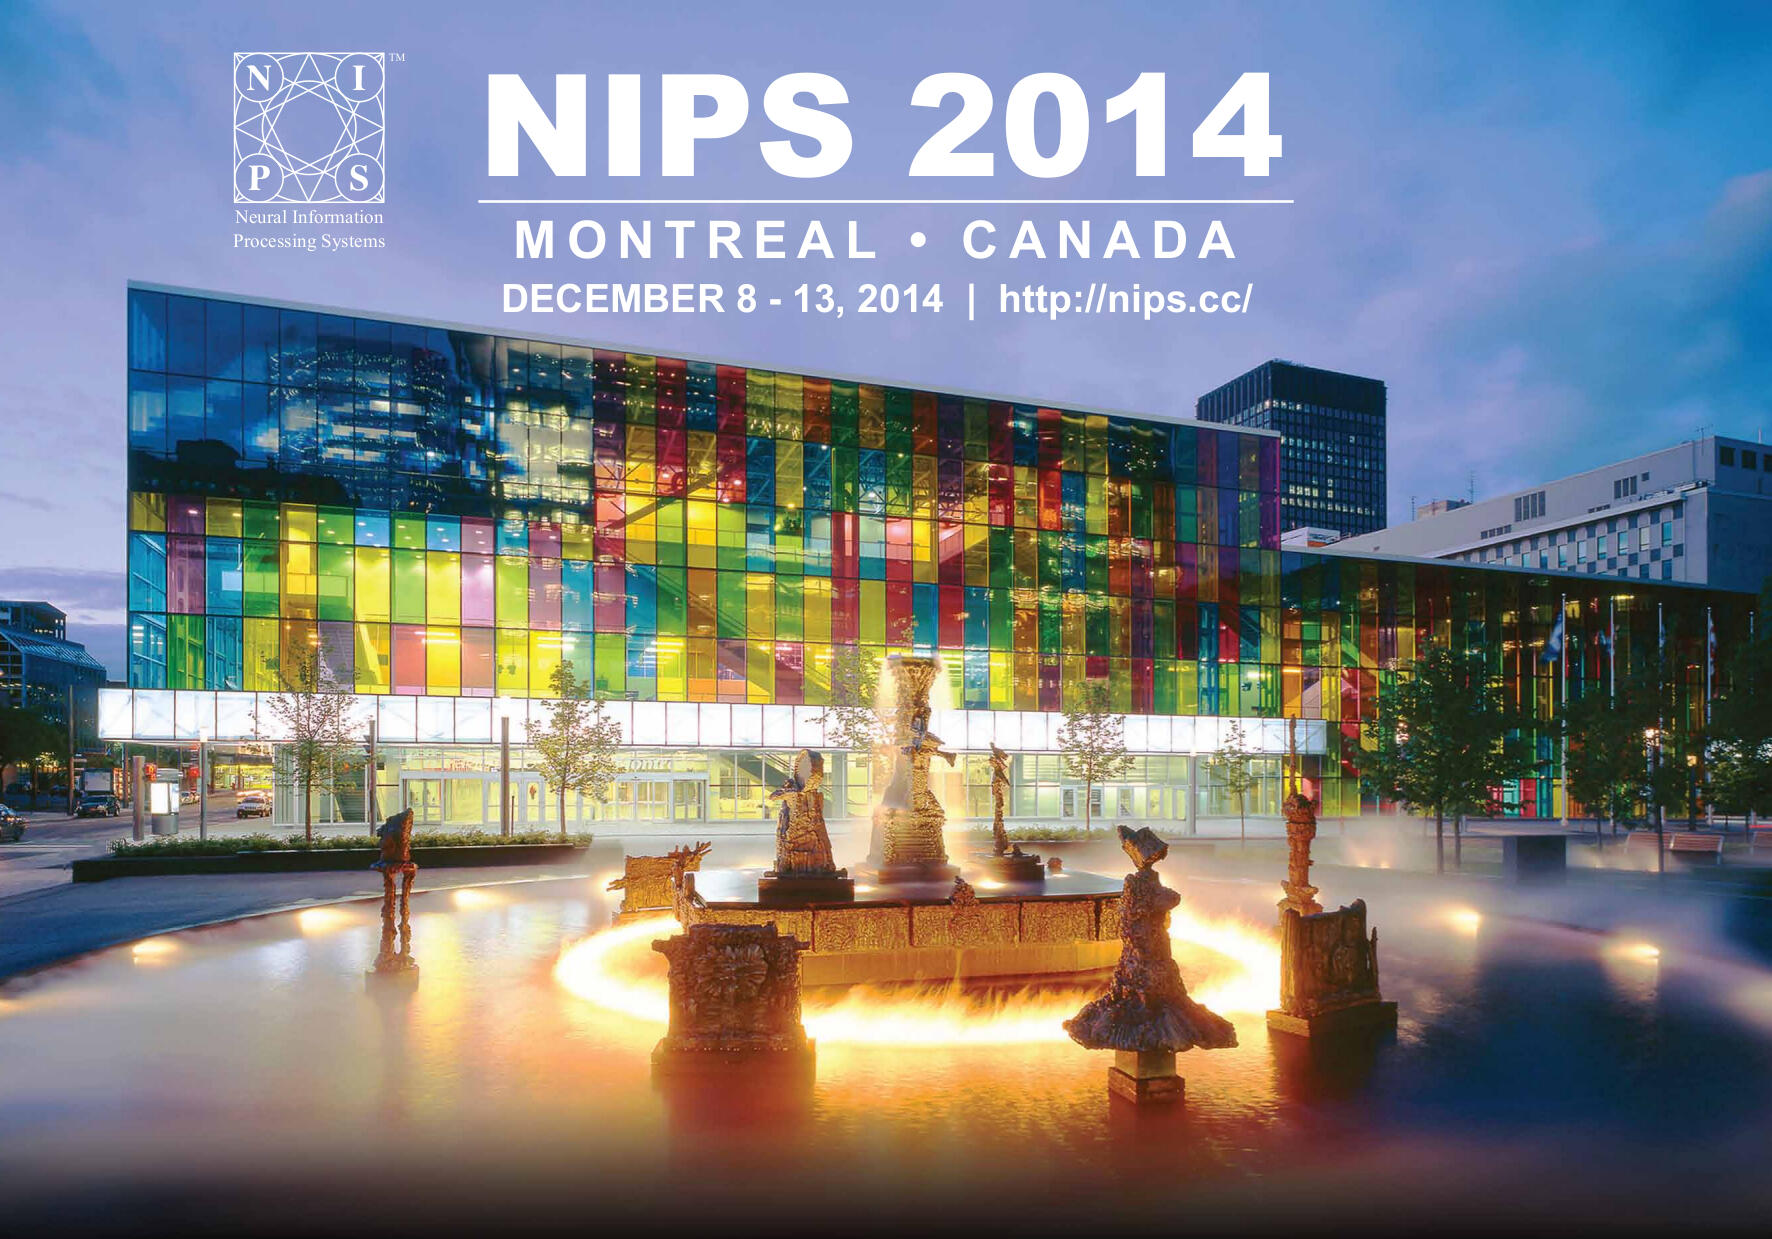
\includegraphics[width=\textwidth]{gtx_exp/nips_poster}
	\end{subfigure}

	\begin{subfigure}[b]{0.32\textwidth}
		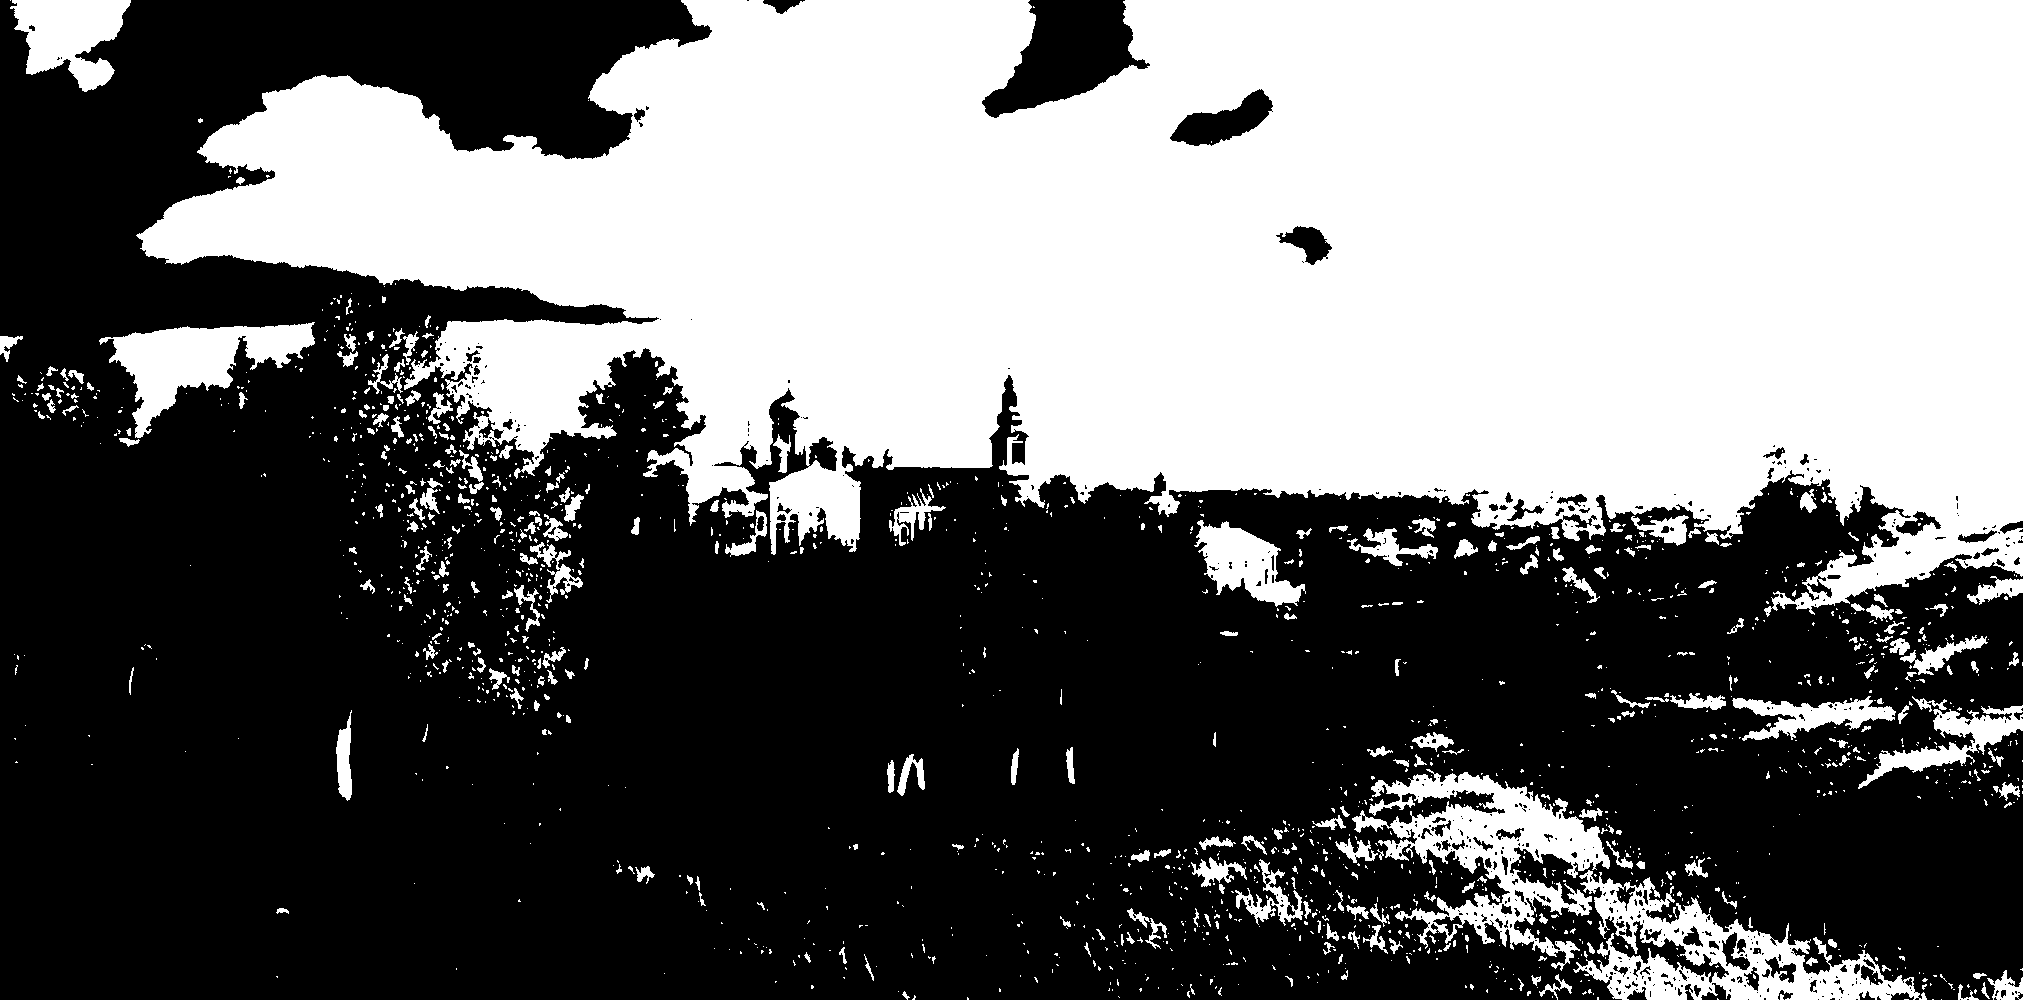
\includegraphics[width=\textwidth]{gtx_exp/zmonastery_bin}
		\caption{monastery}
	\end{subfigure}~
	\begin{subfigure}[b]{0.32\textwidth}
		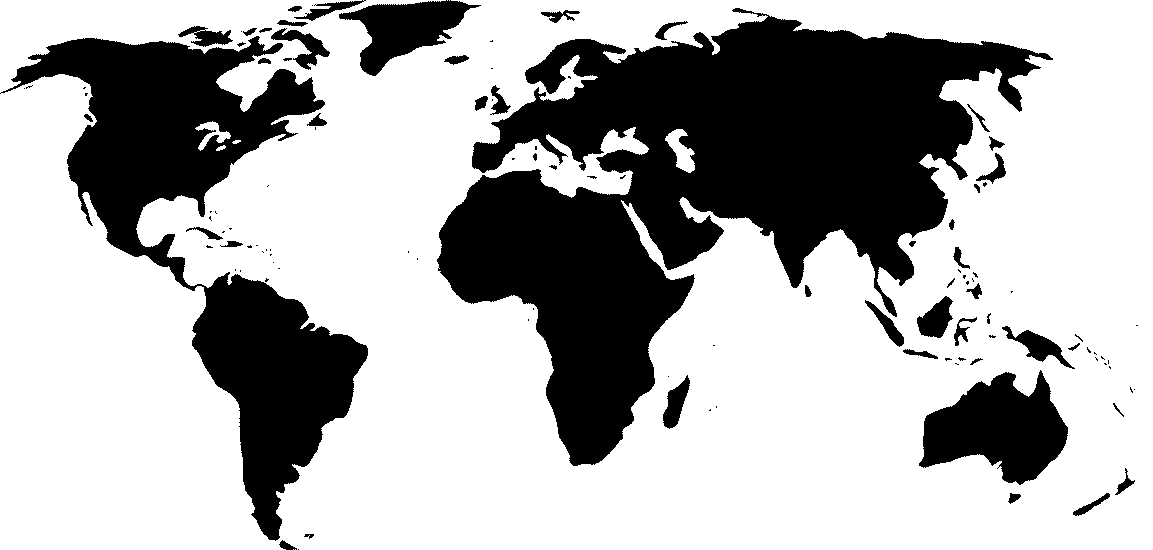
\includegraphics[width=\textwidth]{gtx_exp/zworld_bin}
		\caption{world}
	\end{subfigure}~
	\begin{subfigure}[b]{0.32\textwidth}
		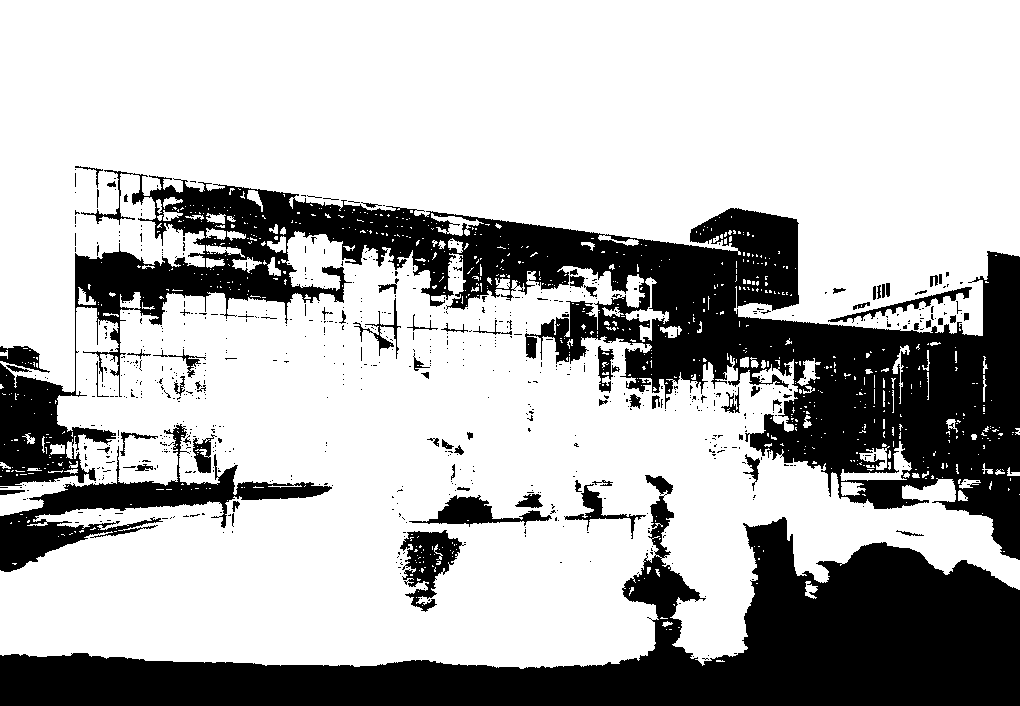
\includegraphics[width=\textwidth]{gtx_exp/nips_poster_bin}
		\caption{poster}
	\end{subfigure}

	\begin{subfigure}[b]{0.32\textwidth}
		
\includegraphics[width=\textwidth]{gtx_exp/nips_logo}
	\end{subfigure}~
	\begin{subfigure}[b]{0.32\textwidth}
		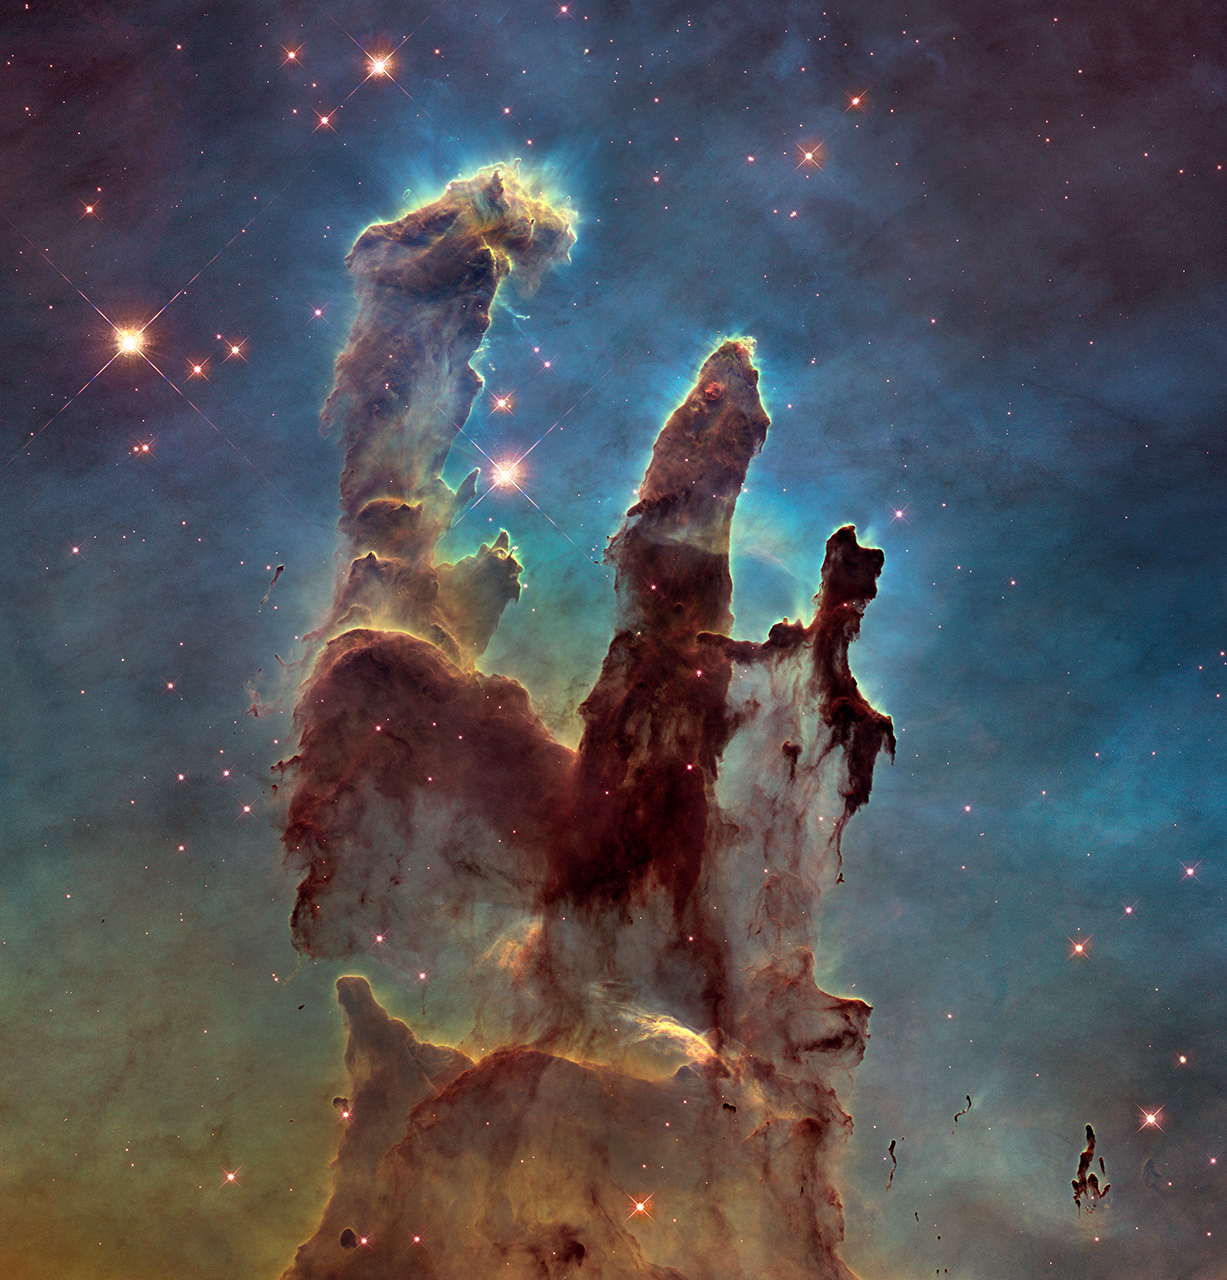
\includegraphics[width=\textwidth]{gtx_exp/space}
	\end{subfigure}~
	\begin{subfigure}[b]{0.32\textwidth}
		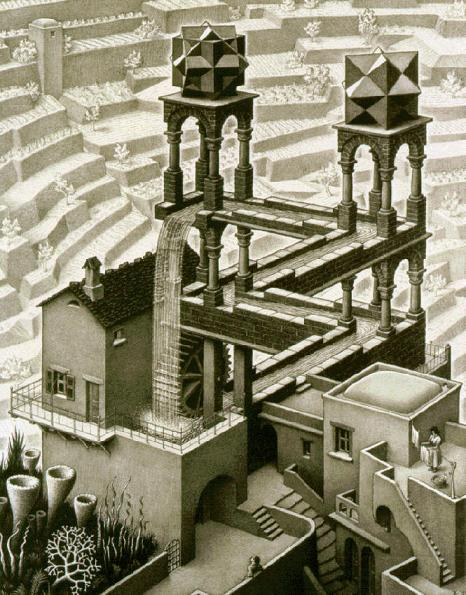
\includegraphics[width=\textwidth]{gtx_exp/waterfall}
	\end{subfigure}

	\begin{subfigure}[b]{0.32\textwidth}
		
\includegraphics[width=\textwidth]{gtx_exp/nips_logo_bin}
		\caption{logo}
	\end{subfigure}~
	\begin{subfigure}[b]{0.32\textwidth}
		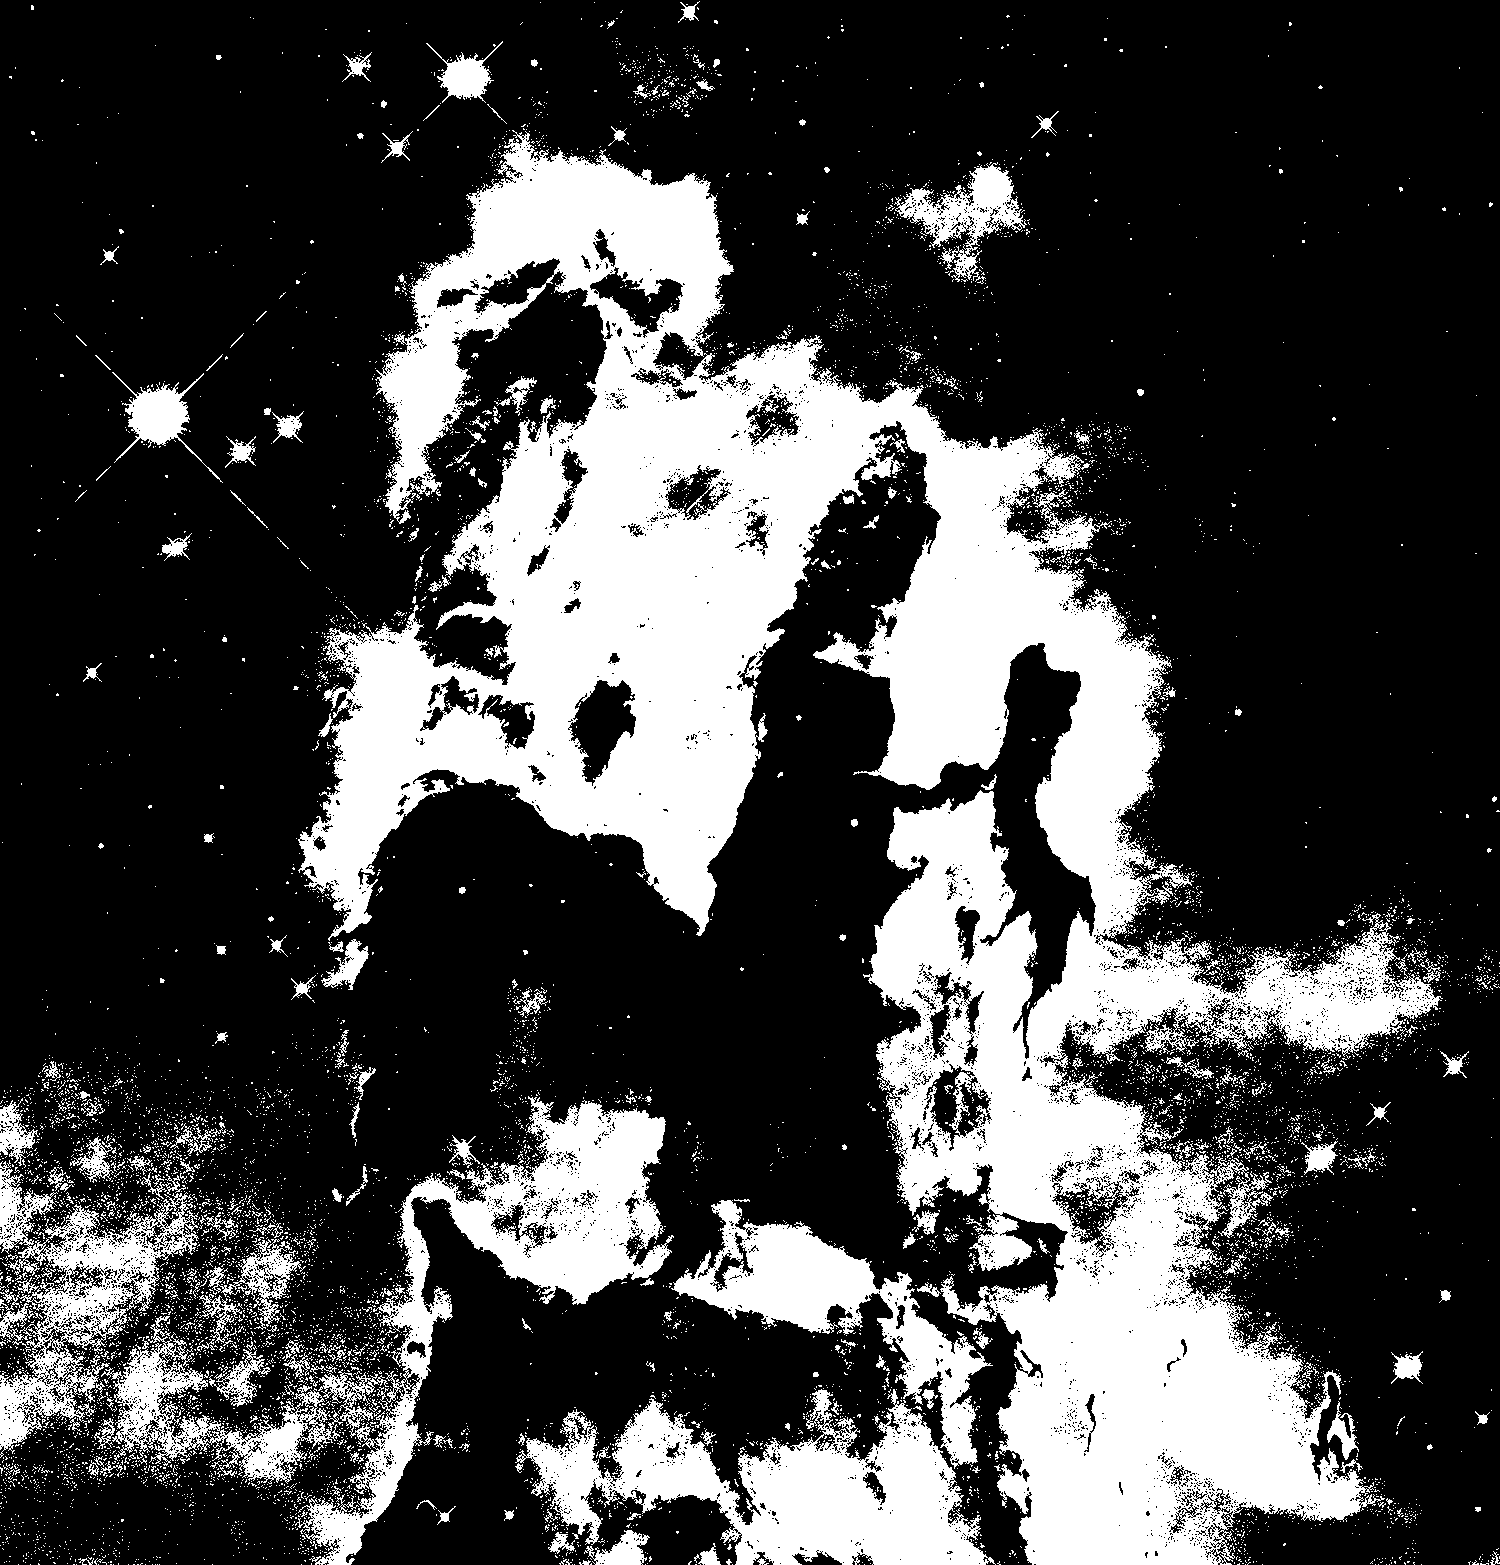
\includegraphics[width=\textwidth]{gtx_exp/space_bin}
		\caption{space}
	\end{subfigure}~
	\begin{subfigure}[b]{0.32\textwidth}
		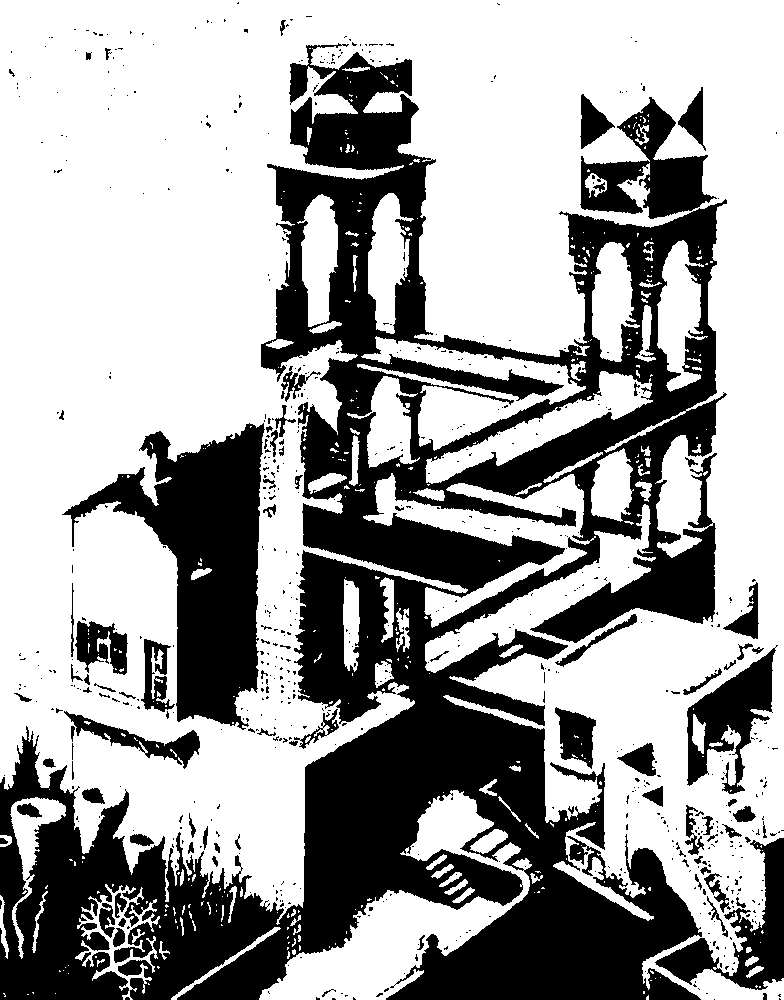
\includegraphics[width=\textwidth]{gtx_exp/waterfall_bin}
		\caption{waterfall}
	\end{subfigure}
	\caption{Real world pictures and their binarized version}\label{fig:gtx_xp_bwpics}
\end{figure}

\subsubsection{Stretch}

The first property of Galaxy trees we wish to evaluate is their stretch, which depends only of graph
topology. Recall that following equation~\autoref{eq:test_stretch_def}, we define the average test
edge stretch as $\frac{1}{|\etest{}|} \sum_{(u,v) \in \etest{}} |\mathrm{path}^T_{u,v}|$,
where $|\mathrm{path}^T_{u,v}|$ is the unique path between $u$ and $v$ in $T$.

As we consider unweighted graphs, we compare \gtx{} with a natural baseline, namely a spanning tree
rooted at the highest degree node and obtained through a breadth first visit of the graph. This
involves randomness in the order in which nodes are visited. Likewise in \gtx{}, the choice of the edge
linking two stars is not always unique, meaning that we have to break ties at random.  Therefore,
for each graph, we repeat the tree construction \np{12} times and present the average result, noting that
the variance (showed as error bar in \autoref{fig:gtx_xp_st}) is small.

On \lpa{} and \triangle{}, we see in \autoref{fig:gtx_xp_st} that both trees exhibits logarithmic stretch, although with a
larger constant for \gtx{}. Note that this is also the case for others low stretch tree methods
\autocite[Section 5.3.1]{papplow}. On \grid{} however, \gtx{} preserves this logarithmic stretch growth
while this is visually no longer the case for \bfs{}.
In that case, we cannot expect a better stretch than $\frac{\log n}{2048}$ according to
\autocite[Theorem 6.6]{LowerBound95}.

\begin{figure}[tbh]
	\centering
	\begin{subfigure}[b]{0.9\textwidth}
		\includegraphics[width=\textwidth]{gtx_exp/gridst}
		\caption{\grid{} }\label{fig:gtx_xp_gridst}
	\end{subfigure}

	\begin{subfigure}[b]{0.9\textwidth}
		\includegraphics[width=\textwidth]{gtx_exp/past}
		\caption{\lpa{} }\label{fig:gtx_xp_past}
	\end{subfigure}

	\begin{subfigure}[b]{0.9\textwidth}
		\includegraphics[width=\textwidth]{gtx_exp/trst}
		\caption{\triangle{} }\label{fig:gtx_xp_trst}
	\end{subfigure}
	\caption{Stretch over graphs of increasing size}\label{fig:gtx_xp_st}
\end{figure}

\subsubsection{Sign prediction}

The second design goal of Galaxy trees is to accurately predict the sign of edges in $\etest{}$.
Except for the three real datasets that already include signs\footnote{We nonetheless perform some
preprocessing in order to make them undirected and to remove the small proportion of conflicting edges
(e.g. positive from $u$ to $v$ but negative from $v$ to $u$).}, all the other are constructed,
meaning we have to set sign on their edges in the first place. This is done by partitioning the
nodes into two clusters. For \gplus{} we use node gender, for pictures we use node color (black or
white), and for all others, we propagate labels $0$ and $1$ from randomly selected high degree nodes.
Once each node belongs to one of the two clusters, we set the sign of an edge between two nodes to
be $+$ if they are in the same cluster and $-$ otherwise.  Predicting using path parity will thus
gives perfect result. To test performance in real situations, we then add noise, that
is we select a fraction of edges uniformly at random and flip their sign. 

Like in \autoref{s:exp}, we evaluate the performance of our prediction using the Matthews
Correlation Coefficient (MCC), defined in equation~\autoref{eq:troll_mcc} \vpageref{eq:troll_mcc}.
As showed in \autoref{fig:gtx_xp_mcc}, when the noise level is low, \gtx{} performs better than
\bfs{}. As the noise level gets higher, they have similar performance. Note also than in
\autoref{fig:gtx_xp_pasynthmcc}, \gtx{} is less sensible to the size of the graph.

\begin{figure}[tbh]
	\centering
	\begin{subfigure}[b]{0.47\textwidth}
		\includegraphics[width=\textwidth]{gtx_exp/grsynthmcc}
		\caption{Synthetic \grid{} }\label{fig:gtx_xp_grsynthmcc}
	\end{subfigure}~
	\begin{subfigure}[b]{0.47\textwidth}
		\includegraphics[width=\textwidth]{gtx_exp/grrwmcc}
		\caption{Pictures \grid{} }\label{fig:gtx_xp_grrwmcc}
	\end{subfigure}
	\begin{subfigure}[b]{0.47\textwidth}
		\includegraphics[width=\textwidth]{gtx_exp/pasynthmcc}
		\caption{Synthetic \lpa{} }\label{fig:gtx_xp_pasynthmcc}
	\end{subfigure}~
	\begin{subfigure}[b]{0.47\textwidth}
		\includegraphics[width=\textwidth]{gtx_exp/trmcc}
		\caption{\triangle{} }\label{fig:gtx_xp_trmcc}
	\end{subfigure}
	\begin{subfigure}[b]{0.47\textwidth}
		\includegraphics[width=\textwidth]{gtx_exp/parwmcc}
		\caption{Real world network }\label{fig:gtx_xp_parwmcc}
	\end{subfigure}
	\caption{MCC over various graphs}\label{fig:gtx_xp_mcc}
\end{figure}

To further assess the quality of our trees, we plug them in them into an existing heuristic method
to predict edge sign: \asym{}~\autocite{Kunegis2009}.
%\Todo{It might also be interesting to see if that would be a good training set for our troll method, although it has to be checked it makes sense from a running time point of view.}
It computes the exponential of the adjacency matrix after it has
been reduce to $z$ dimension. This allows to count the sign of all paths between two pairs of nodes
with decreasing weight depending of their length. To simulate an active learning setting, we reveal
only a subset of edge in $A$. This subset can be: $i)$ the edges forming a \bfs{}, $ii)$ the edges
forming a \gtx{} $iii)$ $|V|-1$ edges chosen uniformly at random.
We set the parameter $z$ equal to $15$ because $i)$ it is one of the best in \cite[Fig.
11]{Kunegis2009} and $ii)$ it performs well on real datasets in \cite[Fig.3]{Cesa-Bianchi2012a}.
% , and $iii)$ it was good in our initial testing (\texttt{20150401\_wed\_spectral.ipynb}).

As the \asym{} has a $O(n^3)$ complexity and uses quite some memory at prediction time, the larger
graphs used previously are not all included. The conclusion of \autoref{fig:gtx_xp_asym} is that
except on social networks, it is better to use spanning trees than random edges. Specifically, \gtx{}
on \grid{} and \bfs{} elsewhere.

\begin{figure}[tbh]
	\centering
	\begin{subfigure}[b]{0.47\textwidth}
		\includegraphics[width=\textwidth]{gtx_exp/grsynthasym}
		\caption{Synthetic \grid{} \label{fig:gtx_xp_grsynthasym}}
	\end{subfigure}~
	\begin{subfigure}[b]{0.47\textwidth}
		\includegraphics[width=\textwidth]{gtx_exp/grrwasym}
		\caption{\enquote{Real} \grid{} }\label{fig:gtx_xp_grrwasym}
	\end{subfigure}
	\begin{subfigure}[b]{0.47\textwidth}
		\includegraphics[width=\textwidth]{gtx_exp/pasynthasym}
		\caption{Synthetic \lpa{} }\label{fig:gtx_xp_pasynthasym}
	\end{subfigure}~
	\begin{subfigure}[b]{0.47\textwidth}
		\includegraphics[width=\textwidth]{gtx_exp/trasym}
		\caption{\triangle{} }\label{fig:gtx_xp_trasym}
	\end{subfigure}
	\begin{subfigure}[b]{0.47\textwidth}
		\includegraphics[width=\textwidth]{gtx_exp/parwasym}
		\caption{Real world network }\label{fig:gtx_xp_parwasym}
	\end{subfigure}
	\caption{\asym{} over various graphs}\label{fig:gtx_xp_asym}
\end{figure}

\iffalse
Finally\marginpars{Actually I never did it because \shz{} wasn't implemented at the time, so now is
a good occasion}\todo*{Run shazoo on galaxy tree} we also compare \gtx{} with \bfs{} and \rst{} on
the task of nodes prediction using \shz{} algorithm~\autocite{Vitale2012}.
\fi


\section{Conclusion}


\begingroup
\newgeometry{hmargin=2cm,vmargin=1.3cm}
\setstretch{0.9}
\todos

\setlength\bibitemsep{2pt}
\printbibliography
\restoregeometry
\endgroup

% \bibliography{/home/orphee/data/projects/biblio/library.bib,more.bib}
% \bibliographystyle{plainnat}
\end{document}
